\documentclass{ieeeaccess}
\usepackage{cite}
\usepackage{amsmath,amssymb,amsfonts}
\usepackage{breqn}
\usepackage{mathtools}
\usepackage{algorithmic}
\usepackage{graphicx}
\usepackage{textcomp}
\usepackage{caption}
\usepackage{subcaption}
\usepackage{float}
\usepackage[flushleft]{threeparttable}
\usepackage{bm}
\usepackage[inline]{enumitem}
\usepackage[hyphens]{url}

% \setcounter{MaxMatrixCols}{30}
% \providecommand{\U}[1]{\protect\rule{.1in}{.1in}}
\newtheorem{theorem}{Theorem}
% \newtheorem{acknowledgement}[theorem]{Acknowledgement}
% \newtheorem{algorithm}[theorem]{Algorithm}
% \newtheorem{case}[theorem]{Case}
% \newtheorem{conclusion}[theorem]{Conclusion}
% \newtheorem{corollary}[theorem]{Corollary}
% \newtheorem{definition}[theorem]{Definition}
\newtheorem{lemma}{Lemma}
% \newtheorem{notation}{Notation}
% \newtheorem{problem}[theorem]{Problem}
\newtheorem{remark}{Remark}
% \newtheorem{solution}[theorem]{Solution}
\newtheorem{assumption}{Assumption}[section]
\newenvironment{proof}[1][Proof]{\noindent\textbf{#1.} }{\ \rule{0.5em}{0.5em}}
\def\BibTeX{{\rm B\kern-.05em{\sc i\kern-.025em b}\kern-.08em
    T\kern-.1667em\lower.7ex\hbox{E}\kern-.125emX}}
    
\begin{document}
% \captionsetup[figure]{labelfont={bf},labelformat={default},labelsep=period,name={Fig.}}

\history{Date of publication xxxx 00, 0000, date of current version xxxx 00, 0000.}

\doi{10.1109/ACCESS.2017.DOI}

\title{Motion Planning and Robust Fault-Tolerant Control of Hybrid UAVs and Biped Robots Team System for Search and Rescue Usage}

\author{\uppercase{Bor-Sen Chen}\authorrefmark{1,2}, \IEEEmembership{Life
Fellow, IEEE}, \uppercase{Ting-Wei Hung\authorrefmark{1}}}

\address[1]{Department of Electrical Engineering, National Tsing Hua
University, Hsinchu 30013, Taiwan} \address[2]{Department of Electrical
Engineering, Yuan Ze University, Taoyuan 32003, Taiwan}

\tfootnote{This work was supported by the Ministry of Science and Technology
of Taiwan under Grant MOST 108-2221-E-007-099-MY3.}

\markboth
{Author \headeretal: Preparation of Papers for IEEE TRANSACTIONS and JOURNALS}
{Author \headeretal: Preparation of Papers for IEEE TRANSACTIONS and JOURNALS}

\corresp{Corresponding author: Bor-Sen Chen (bschen@ee.nthu.edu.tw)}
% \address[1]{National Institute of Standards and 
% Technology, Boulder, CO 80305 USA (e-mail: author@boulder.nist.gov)}
% \address[2]{Department of Physics, Colorado State University, Fort Collins, 
% CO 80523 USA (e-mail: author@lamar.colostate.edu)}
% \address[3]{Electrical Engineering Department, University of Colorado, Boulder, CO 
% 80309 USA}
% \tfootnote{This paragraph of the first footnote will contain support 
% information, including sponsor and financial support acknowledgment. For 
% example, ``This work was supported in part by the U.S. Department of 
% Commerce under Grant BS123456.''}

% \markboth
% {Author \headeretal: Preparation of Papers for IEEE TRANSACTIONS and JOURNALS}
% {Author \headeretal: Preparation of Papers for IEEE TRANSACTIONS and JOURNALS}

% \corresp{Corresponding author: First A. Author (e-mail: author@ boulder.nist.gov).}
% .

\begin{abstract}
In this study, we investigate a motion planning and robust fault-tolerant control of a hybrid UAVs and biped robots team system (URTS) for the purpose of search and rescue (S\&R). The system architecture of URTS is proposed at first to illustrate the issues to be addressed in URTS and the relationships between them. The task allocation and path planning problems are first investigated and stated. Next, we focus on the local motion planning problem for UAV flying and robot walking behavior, and then the tracking control problem for UAV and robot. The relationship between local motion planning and tracking control, the transformation of the reference trajectory, is also explored in detail. By converting the dynamics model of UAV and robot into a unified agent dynamics model, a design method for an robust $H_\infty$ decentralized observer-based feedforward-linearized PID fault-tolerant control (FTC) is proposed for the agents in URTS. A novel smoothing signal model of fault signal is embedded into the linearized system to achieve the active FTC through observer estimation. Then, the design of the robust $H_\infty$ decentralized observer-based feedforward-linearized PID FTC of URTS is transformed into a linear matrix inequality (LMI) -constrained optimization problem which can be solved by a two-step design procedure. With the help of MATLAB LMI Toolbox, the tracking problem of each UAV and robot in URTS is effectively solved. Finally, the simulation results are used to demonstrate the operation of URTS and to verify the effectiveness of the proposed tracking control method under the external disturbance and the actuator and sensor fault.
\end{abstract}

\begin{keywords}
biped robot, fault-tolerant control, heterogeneous multi-agent system, robust $H_\infty$ control, S\&R, smoothing signal model, UAV, hybrid UAVs-UGVs team system
\end{keywords}

\titlepgskip=-15pt

\maketitle

\section{Introduction}
% unmanned vvehcile
\PARstart{I}{n} recent years, the unmanned vehicle (UV) has attracted attention due to the advances in communication technology, sensing devices, and computing power. It not only reduces labor costs and brings convenience to life, but more importantly, it can replace some dangerous jobs for humans. Due to these benefits, it has been widely used in many scenarios, such as S\&R, battlefield, logistics and transportation, surveillance, etc \cite{9700861}. Compared with a single UV, multiple UVs can perform more complex tasks and are more robust due to a large number of agents \cite{8352646}. However, the cost is that the design of such a multi-agent system (MAS) becomes more intricate as there are more problems to be resolved, such as formation, collision avoidance between agents, task allocation, and cooperation between agents \cite{chen2019control}. In addition to the number increasment, a heterogeneous multi-agent system (HMAS) combining various types of UV is also valued \cite{9371292}. Compared with homogeneous multi-agent system, it can adapt to a wider variety of application scenarios because each agent has different aptitudes.

To construct an unmanned HMAS, the three required key capabilities are perception, decision-making and control. Perception is to obtain information through the sensor (e.g., localization or computer vision), decision-making is to make decisions through the sensor information, and control is to execute the decision through the actuator. To limit the scope of this paper, we focus on decision-making and control problem only. Three main problems of decision-making in an unmanned HMAS are task allocation, path planning and collision avoidance. Task allocation is to optimally assign tasks to each agent under some constraints such as agent capabilities, fuel cost, time cost, etc \cite{skaltsis2021survey}. Path planning is to optimally plan paths for each agent while subject to constraints such as agent kinodynamic properties, distance, obstacles collision, etc \cite{zhang2018path}. Collision avoidance is to avoid collision with obstacles. Although collision avoidance is often concerned in path planning, the collision avoidance system is also independently studied because of the requirements for the safety and reliability of the actual system \cite{9108245}.

Although there are many types of UVs to make up an unmanned HMAS, Unmanned Aerial Vehicle (UAV) and Unmanned Ground Vehicle (UGV) have been the subject of major recent research because of their availability and applicability. Additionally, the complementarity between them also makes such a system more potential \cite{arbanas2018decentralized}. In other words, UAV is widely used in reconnaissance due to the high mobility. However, the carrying capacity of UAV is very low compared to UGV since there is no ground support. In contrast, UGV has higher carrying capacity but is easily restricted by ground obstacles and cannot move at high speed. For these reasons, a hybrid UAVs-UGVs team system will be more appealing. To discuss more concretely, we consider a hybrid UAVs-UGVs team system for S\&R. For the need for search mobility, we choose quadrotor aircraft as UAV. In order to deal with the complex terrain of the S\&R environment, we choose biped robot as UGV. Even though other types of UGVs like wheeled robots and vehicles are easier to handle than biped robot, the high degree of freedom and the compatibility of the human environment still makes it a good candidate of UGV in a S\&R system.

To the best of the authors' knowledge, most of the literature focus on only one specific problem in such an unmanned multi-agent S\&R system, such as task allocation problem, path planning problem or control problem. Additionally, few literatures illustrate the relationship between these problems. This leads us to propose a system architecture of hyibrid UAVs and biped robots team system (URTS) for S\&R usage. The flowchart of decision-making and control process of URTS is also given. We divide it into five main hierarchical processes, i.e., task allocation, path planning, behavior layer, local motion planning and tracking control. It is because the URTS needs to be able to assign different tasks to agents to perform first. After a task is assigned, if the task is to reach a goal location, a path to reach it needs to be planned. To make agent move on the path, a behavior corresponding to the environment is required to determine. Then, a local motion corresponding to the behavior of the agent needs to be designed. Finally, a controller must be designed to track the trajectory of the motion. In order to further limit the scope of the study, we will focus on the latter two processes. But to illustrate how the whole system works, the first three problems are also briefly stated.

% To discuss the local motion planning problem and tracking control problem, the real mechanical system for each agent corresponds must be considered. To meet the need for search mobility, we choose quadrotor aircraft as UAV. The control problem of UAV has been widely studied due to its applicability and low cost (cite: uav control). In order to deal with the complex terrain of the S\&R environment, biped robot was chosen as the UGV. Although other types of UGVs like wheeled robots and vehicles are easier to handle than biped robot, the high degree of freedom and the compatibility of the human environment still makes it a good candidate of UGV in a S\&R system. However, to let the biped robot moving, not only the control problem (cite: robot control) but also the local motion planning problem need to be solved. The local motion planning of the walking of biped robot, i.e., stable walking pattern generation, is discussed in this paper. Related researches can be found in (cite: walking pattern).

The local motion planning is the bridge between path planning and tracking control since the path found by path planning algorithm and the path enforced to follow by a controller are not necessarily the same. The reason is that path planning algorithm usually treats the agent as a point, while the actual agent in the physical world is a mechanical system for the tracking control design. A mechanical system means that there exist kinodynamic constraints. This makes certain paths impossible to follow for an actual agent, such as paths that are not smooth, have too large curvature, or require too large velocity and acceleration. Although some literatures directly tackle the kinodynamic constraints path planning problem \cite{9384209}, this paper splits path planning into three steps, i.e., (i) path planning, (ii) behavior layer and (iii) local motion planning for clarity. Through this decomposition, we can focus on the local motion planning of specific behaviors. The local motion planning of flying behavior for UAV and walking behavior for robot is studied in this paper, especially the latter. The local motion planning of biped robot walking, i.e., stable walking pattern generation, is a popular research topic due to its challenge \cite{olcay2017design}.

The tracking control is to control an agent to follow a desired trajectory. There are many control strategies for MAS. According to the way of the design of controller, it can be divided into centralized control and decentralized control in control field \cite{8931370}. Centralized control means there exists a powerful central controller in MAS to gather the state information of MAS and send the control command back to each agent to reach a global goal. Due to the powerful nature of the central controller, control commands can be determined well and quickly. But when it fails, the whole system will be completely paralyzed. In contrast, decentralized control means that each agent has its own controller to collect and control the agent's own state information. Under this architecture, although the global goal cannot be achieved, the possibility of paralyzing the entire system due to the failure of the controller can be avoided.

Besides, the formation control is also a topic in MAS \cite{wang2022consensus}. Its purpose is to keep a MAS in a formation while moving. Although formation control provides a simple framework for the control of a large number of agents, considering the complexity of the disaster relief environment, formation will make the application of URTS inflexible. It is because we expect that agents in URTS need to organize multiple teams of different scales and types to deal with multiple tasks of different scales and types in a disaster relief environment. In this situation, it is more reasonable to treat each agent as an independent individual and specify an independent trajectory for each agent to follow.

In order to cope with the fault in the actual system, the fault-tolerant control (FTC) has also been widely studied. According to the way of handling the fault, it can be divided into the passive FTC and the active FTC \cite{6669235}. The passive FTC treats the fault as an unknown system perturbation and designs a control law to tolerate it. In contrast, the active FTC will first estimate and identify the fault and then compensate it through the controller. Despite the added complexity in controller design, the active FTC will outperform the passive FTC due to the extra estimation steps. Based on the foregoing, a robust $H_\infty$ decentralized observer-based feedforward-linearized PID FTC is proposed to deal with the control problem in URTS.
% The control problem of UAV has been widely studied due to its applicability and low cost (cite: uav control).
% the control problem of robot

The contributions of this study are described as follows:
\begin{enumerate}
    \item A system architecture and system flow of URTS for the purpose of S\&R are proposed so that the issues involved in URTS and their relationships can be defined and resolved.
    \item A transformation between the trajectory generated by the path planning algorithm and the trajectory required for tracking control design is proposed to enable some common path planning algorithms can be applied to the tracking control of agents in URTS.
    \item A general agent dynamics model is proposed so that the robust $H_\infty$ decentralized observer-based tracking control problems of the heterogeneous agents in URTS, UAVs and biped robots, can be solved together.
\end{enumerate}

The remainder of the paper is organized as follows. In Section II, a system architecture of URTS in S\&R usage is proposed and the function and relationship of its components, i.e., task allocation, path planning, behavior layer, local motion planning and tracking control are described. In Section III, the system model of agents in URTS are given to design the motion of UAV flying and biped robot walking behavior and the control strategy of agents. In Section IV, a robust $H_\infty$ decentralized observer-based feedforward-linearized PID FTC is proposed for the agents in URTS with the help of a general agent dynamics model. In Section V, a simulation example is given to illustrate the operation of the system architecture of URTS and to verify the effectiveness of the proposed tracking control method. In Section VI, a conclusion is maded.

\textbf{Notation 1:} 
$diag(A_1, A_2, \dots, A_n)$: a block diagonal matrix with main diagonal blocks $A_1, A_2, \dots, A_n$. $A^T$: transpose of $A$. $A > 0$: a positive definite matrix. $(a_n)$: a sequence. $(a_{k_n})$: a subsequence of a sequence $(a_n)$. $[a_{j,k}]$: A matrix with the entries $a_{j,k}$ in the $j$th row and $k$th column. $\vert{S}\vert$: size of a set $S$. $\otimes$: Kronecker product. $I_n$: n-dimension identity matrix. $x(t)\in L_2\begin{bmatrix}
    0,t_f 
\end{bmatrix}$ if $\int^{t_f}_{0}x^T(t)x(t)dt<\infty$. $Sym(A)$: sum of a matrix $A$ and its tranposed, i.e., $Sym(A) = A+A^T$.

\section{PRELIMINARIES OF URTS in S\&R usage}
The URTS will start with a given S\&R area, and end with mission completed. The URTS is composed of $N_T$ teams and a ground station. Each team contains $N_A$ agents with $1$ UAV and $N_A-1$ robots. Hence, the $j$th agent in the $i$th team is denoted as $\alpha_{i,j}$, where $i=1,2,...,N_T$ and $j=1,2,...,N_A$. The UAVs are chosed as the first agents in each team, i.e., $\alpha_{i,1}$. Each agent has environmental sensing capability and load capability, while the ground station is responsible for computing and decision-making. Besides, there are communication channels between agents and ground station through wireless network.
% The system architecture if URTS is shown in Fig. \ref{fig:1}.
% \begin{figure}[htbp]
% \centering
% 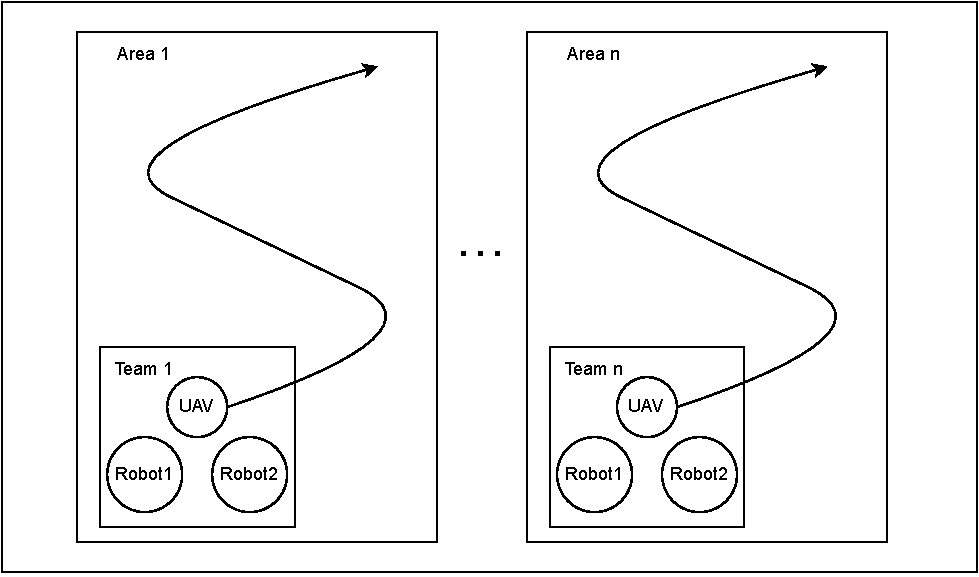
\includegraphics[width=0.4\textwidth]{fig/1.pdf}\caption{System structure of URTS}%
% \label{fig:1}
% \end{figure}

To complete search tasks, each team is designed to be responsible for a small area of the overall S\&R area, and each agent will be assigned an appropriate path to cover the area. To complete rescue tasks, whenever a goal (e.g., victims or disaster area) is found by the machine vision of nearby agent, the ground station will assign some agents to the location of goal. 
% It can be expected that there has multiple search or rescue tasks need to be performed at the same time but there has multiple agents. If each agent can only perform one task at a time, then there exist many feasible way of task allocation. Usually we want this allocation to be optimal, which can be achieved by solving the dynamic task allocation problem.

If a task is to reach a location of certain goal, we need to find a collision-free path to reach it. 
% there must exist multiple feasible paths. Similar to task allocation, we usually want to find an optimal path. 
% Besides, it's necessary to concern about collision between agents or between agents and obstacles in the actual scenario, 
Hence, each agent will also sense distance-related information about its surrounding and send it back to the ground station. The ground station will combine this information with the goal location assigned by task allocation algorithm and make a decision to avoid obstacles and other agents nearby.
% That is, the path of each agent will be reassigned every moment if needed by solving the dynamic path planning problems.

We need to determine specific behavior to follow the path found by path planning algorithm according to the situation of the environment especially for agents with complex mechanical systems like robots. Since such a system has a high degree of freedom, there are many ways to follow the same path (e.g., a robot can walk or run to follow the same path). Furthermore, agents in URTS are not always following the path. Sometimes they need the behavior such as stop to look around, get supplies and put supplies. To meet these needs, a behavioral layer is necessary.
% The behavior layer decides an appropriate behavior based on the circumstances.

In order to make a behavior, we must design a corresponding motion by local motion planning. The motion is a prescribed reference trajectory for an actual mechanical system to follow. Finally, a tracking controller is designed for each agent to follow this desired reference trajectory.

The agents overall have the same system architecture in URTS except for some subprocess differences. Followed by the concept in \cite{paden2016survey}, a system architecture for an agent employed for S\&R is proposed as shown in Fig. \ref{fig:sys}. The Simultaneous Localization And Mapping (SLAM) block converts sensor information into the location of agents $q_{start}$ and an occupancy map $\mathcal{C}$. The visual object recognition block provides distance information and object information through the analysis of sensor information. The object information provides agent machine vision that enables it to determine an appropriate behavior (e.g., a robot can see an obstacle and decides to climb through it). The detailed functions of remaining 5 blocks, i.e., Task Allocation, Path Planning, Behavior Layer, Local Motion Planning and Tracking Control, will be explained in the following subsections.

% To determine the behavior, agent needs the information about environment. The sensing data which include external environment information and internal system information is feedback to Behavior Layer to assist in judging the present state (fig:system). 

\begin{figure}[htbp]
\centering
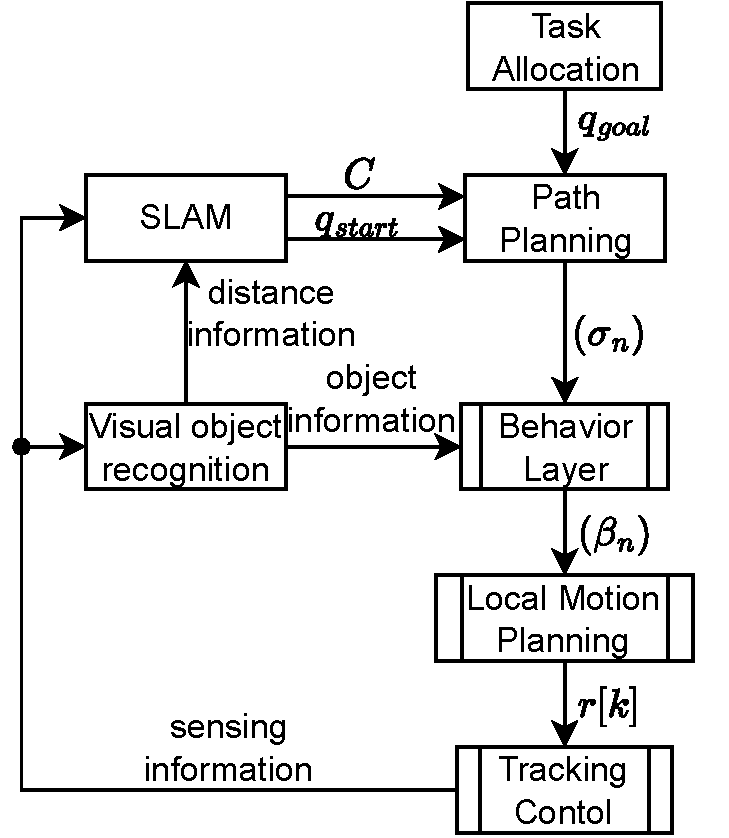
\includegraphics[scale=.15]{fig/sys.png}\caption{The system architecture of agent in URTS. The 2 blocks on left hand side are used to convert the low-level sensor information into high-level information, such as map, start point and object information. The 5 blocks on right hand side are the flow of an agent performing a S\&R mission. From the top to the bottom, it is the decision of the task position, the planning of the path, the decision of the behavior, the planning of the local motion trajectory, and the low-level tracking control.}%
\label{fig:sys}
\end{figure}

\subsection{Task Allocation}
In the URTS, it can be expected that each agent $\alpha_{i,j}$ will be assigned several specific tasks, such as searching a specific area, or delivering supplies to disaster area, etc. However, the number of agents and tasks is more than one, and each agent has different capabilities (e.g., moving speed or load capacity) and status (e.g., their own position or the amount of supplies carried), and each task has different characteristics (e.g., urgency, position, amout of supplies needed). Therefore, the results of task allocation can be "good or bad", which leads us to find the optimal allocation. This problem is referred to a task allocation problem or multi-robot task allocation problem. A problem formulation and a mathematical model of problem can be found in \cite{khamis2015multi}. Although many different formulations and models have been employed to solve the task allocation problem, the common goal is to find a set of agent-task pairs to achieve a specific cost function. In this paper, we assume that the tasks have been properly assigned so that every agent knows a destination $q_{goal}$ it needs to go at every moment.
% $(\mathcal{G})_n, n\in\mathbb{Z}\cap[1, N], N\in\mathbb{Z}^+$
\textit{
    \begin{remark}
        This block is like a commander since it is used to assign task for agents. Thus, if the real S\&R system has human experts as commanders, he can replace its job or make decisions together with it to maximize the rescue value.
    \end{remark}
}
\textit{
    \begin{remark}
        Although each agent has its own team, agents can also work across teams. For example, if the result given by the task allocation algorithm contains the agent-task pairs $(\alpha_{1,5},T_1)$ and $(\alpha_{2,2},T_1)$, then the agent $\alpha_{1,5}$ in team 1 and the agent $\alpha_{2,2}$ in team 2 will execute task $T_1$ together. 
    \end{remark}
}

\subsection{Path Planning}
After a destination $q_{goal}$ is assigned for each agent, next step is to find a collision-free path from current position to it. There must exist multiple feasible paths to go. Similar to task allocation, we usually want to find an optimal path. There are several path planning algorithm to handle this problem. Due to the developmental and universal nature of roadmap-based path planning algorithm, this paper considers it as the path planning method of URTS. This method attempts to discretize the search space into interconnected roads and find the path on it. 
% According to the roadmap construction method, it can be divided into deterministic and sample-based. 

According to the way of pathfinding, it can be divided into multi-query planner and single-query planner \cite{elbanhawi2014sampling}. Multi-query planner will first construct a roadmap and then use a graph search method on it to query the best path, such as Probability Road Map (PRM), Visibility Graph, and Voronoi Diagrams \cite{liu2018survey}. Single-query planner will complete the pathfinding by constructing and querying simultaneously,
%  i.e., the roadmap will be constructed incrementally and toward the goal, 
such as Rapidly-exploring Random Tree (RRT), Expansice Space Tree (EST), and Ariadne's Clew \cite{elbanhawi2014sampling}. However, the environment is dynamic rather static for URTS so some extra structures need to impose on the aforementioned planner. Some common dynamic planners can also be found in \cite{elbanhawi2014sampling}, such as PRM with D* search algorithm, dynamic RRT, and extended RRT. All of the above common roadmap-based planners can be applied to the URTS.

\begin{remark}
    To avoid agents colliding with each other, the concept of multi-agent path planning is proposed \cite{yu2013multi}. However, URTS operates in a large environment so the probability of collision is small and the agents have the ability to communicate. Therefore, when the paths collide, the mechanism of waiting for the other side to pass can be used to avoid the collision problem.
\end{remark}

Furthermore, the constraints imposed by the mechanical structure are needed to consider within pathfinding process mentioned by other literatures but it will be left to local motion planning block to deal with. The reason is that URTS works on a complex environment and therefore requires a variety of behaviors to respond, and different behaviors have different constraints (e.g., curvature constraints between running and walking behavior are expected to be different for robot). In this case, a unified planner will become overly complex and impracticable. Therefore, we divide path planning into three subprocesses, i.e., path planning, behavior layer and local motion planning. The path planning block becomes a global planner and regard an agent as a point without kinodynamic constraints. The local motion planning block becomes a local planner and consider the motion planning of a specific behavior.
% In this case, the configuration space $\mathcal{C}$ degenerates to $\mathbb{R}^3$.

By treating a roadmap-based path planning algorithm as a black box, the output is a sequence (or sayed waypoints), and the three inputs are current configuration $q_{start}$, goal configuration $q_{goal}$, and configuration space $\mathcal{C}$. Current configuration is obtained by GPS, inertial measurement unit, or other locating techniques. Goal configuration is obtained by the previous block, task allocation block. Configuration space $\mathcal{C}$ is constructed by environment information through sensors of agents online or in advance by human knowledge offline. $\mathcal{C}$ is a space containing all possible configurations of agents which are composed of free space $\mathcal{C}_{free}$ and obstacle space $\mathcal{C}_{obs}$, where $\mathcal{C}=\mathcal{C}_{free}\cup\mathcal{C}_{obs}$ and $\mathcal{C}_{free}\cap\mathcal{C}_{obs}=\emptyset$. For a simpler explanation of how the URTS works, the following assumptions are made.

\begin{assumption}
    The locating ability of the URTS is perfect so every agent can know its current configuration $q_{start}$.
\end{assumption}
\begin{assumption}
    A Task Allocation algorithm is already designed so that every agent can know its goal configuration $q_{goal}$.
\end{assumption}
\begin{assumption}
    The URTS is supposed to have a perfect real-time mapping ability so a real-time configuration space $\mathcal{C}$ can be obtained.
\end{assumption}
\begin{assumption} \label{asm:collision} % UAV do not consider obstacle collisions a little wierd.
    UAVs do not consider obstacle collision, so the path of UAVs can be directly assigned rather than found by planner. Robots do not consider obstacle collision in the direction perpendicular to the ground. 
\end{assumption}

From above assumptions, a path of agent can be expressed as a sequence
\begin{equation}
    (\sigma_n), n\in\mathbb{Z}\cap[1,k_f], \sigma_n\in\mathcal{C}
\end{equation}
where $k_f$ is the time step when reaching goal. Since the path planning is dynamic, $(\sigma_n)$ is composed of multiple segments actually. Let $(\sigma_{k_n})$ be the subsequence of $(\sigma_n)$, where $k_n$ is the time step when a replanning decision is occured. Then, the segments of path from the result of the replanning in time step $k_n$ can be expressed as sequences $(\sigma_m), m\in\mathbb{Z}\cap[k_n, k_{n+1})$. For agents, the replanning decision can be due to a goal changing that is made by human or task allocation block. For robot, it can be a collision detected by a dynamic roadmap-based planner. The resulting path $(\sigma_n)$ is passed to the next block, Behavior Layer.

\subsection{Behavior Layer}
% Since UAVs and robots are real physical systems, they must interact with the environment through a behavior so that they can move and act in the physical world.
Path planning tells agents where to go but not how since we regard the agent as a point. Taking robot as an example, it may walk, run, climb, or jump to follow the path $(\sigma_n)$ in real scenario. These behaviors with changing position are classified as "moving" behavior in this paper. Besides, the agents in the hybrid URTS do not always moving. Somtimes they have to suspend to take an action (e.g., getting and putting supplies, rotating in place to collect more environment information) or deal with some unexpected situations (e.g., no path found, the robot falls). These behaviors without changing position are classified as "action" behavior in this paper. More behaviors can be added so that the agent can have more ways to act with environment but there must have a corresponding behavior every moment otherwise the agent will lose control. The sequence of these behaviors can be expressed as:
\begin{equation}
    (\beta_n), n\in\mathbb{Z}\cap[1,k_f], \beta_n\in\mathcal{B}
\end{equation}
where $\mathcal{B}$ is the set of behaviors. It is to say that the path $(\sigma_n)$ is divided into many segments and each segment corresponds to a specific behavior. By the object information in Fig. \ref{fig:sys}, an appropriate behavior can be judged. However, it will be a rather complicated project, so this article only gives the structure of the behavior set. The behavior set $\mathcal{B}$ of agent in URTS can be roughly discribed in Fig. \ref{fig:behavior}.

\begin{figure*}[htbp]
    \centering
    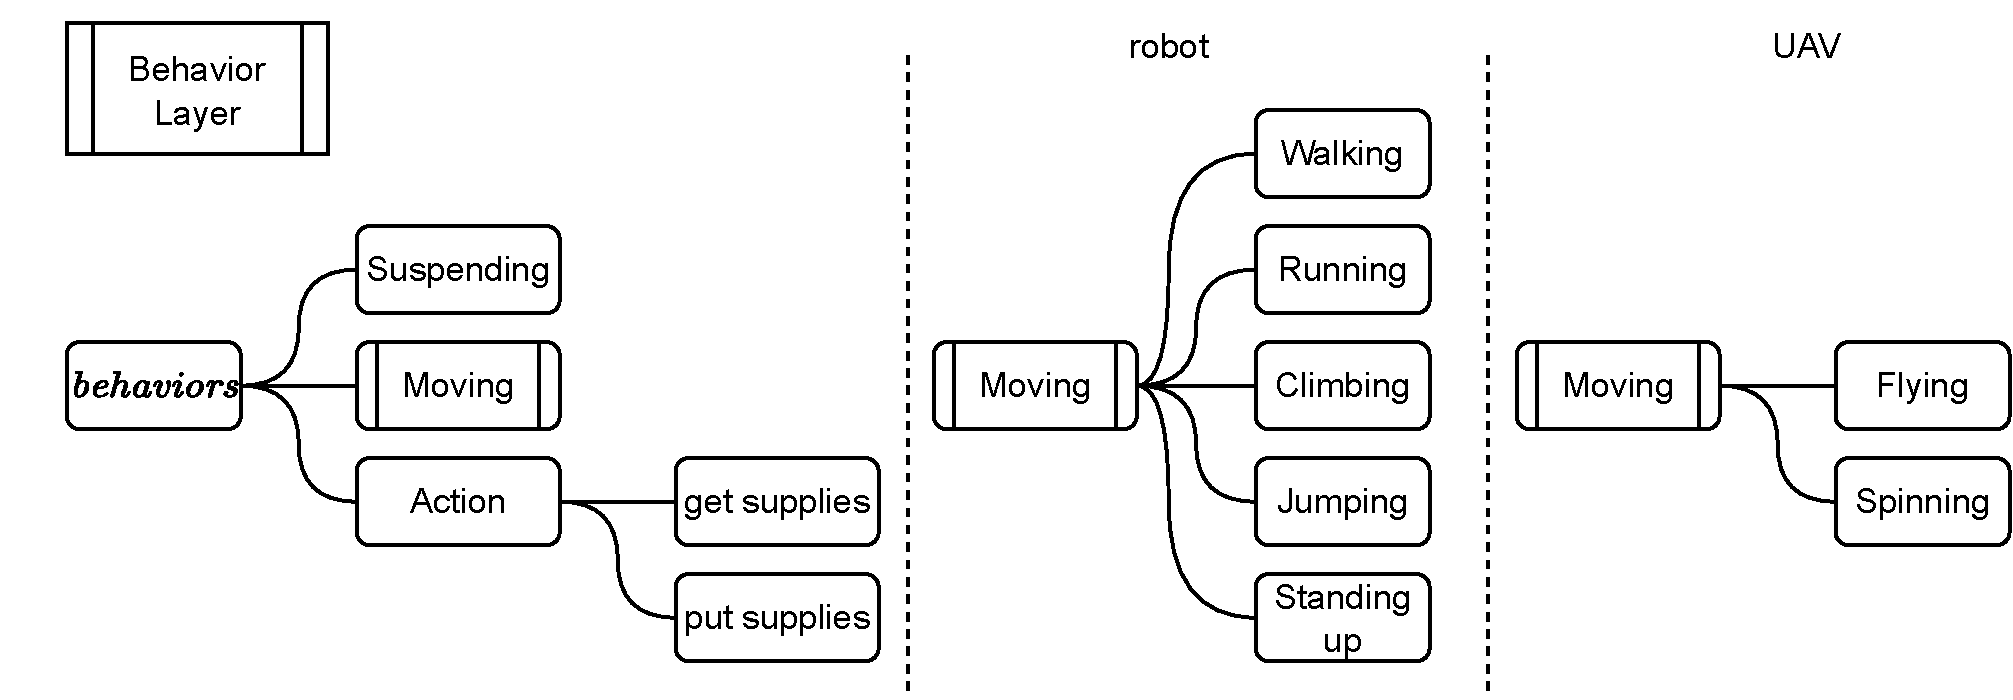
\includegraphics[scale=.12]{fig/behavior.png}\caption{The structure of behavior layer. The leaves of the tree structure are the possible behaviors an agent can take. The behavior to be took at every moment will be decided in this block.}%
    \label{fig:behavior}
\end{figure*}

\subsection{Local Motion Planning}
After a specific behavior is determined, the next step is to design a motion to achieve that behavior. Local motion planning block is like path planning block but its scale is smaller and its resolution and precision must be higher. Collision checking is needed since we consider agent as a point in path planning block and it is a real mechanical body here. Furthermore, the kinodynamic constraint is handled in this block. Although motion planning and path planning are separated into two blocks, the technologies involved are similar and often with the same notion in other literature. Therefore, the output of this block is also a path $r[k]$. The flowchart of local motion planning block is shown in Fig. \ref{fig:LocalMotionPlanning}
\begin{figure*}[htbp]
    \centering
    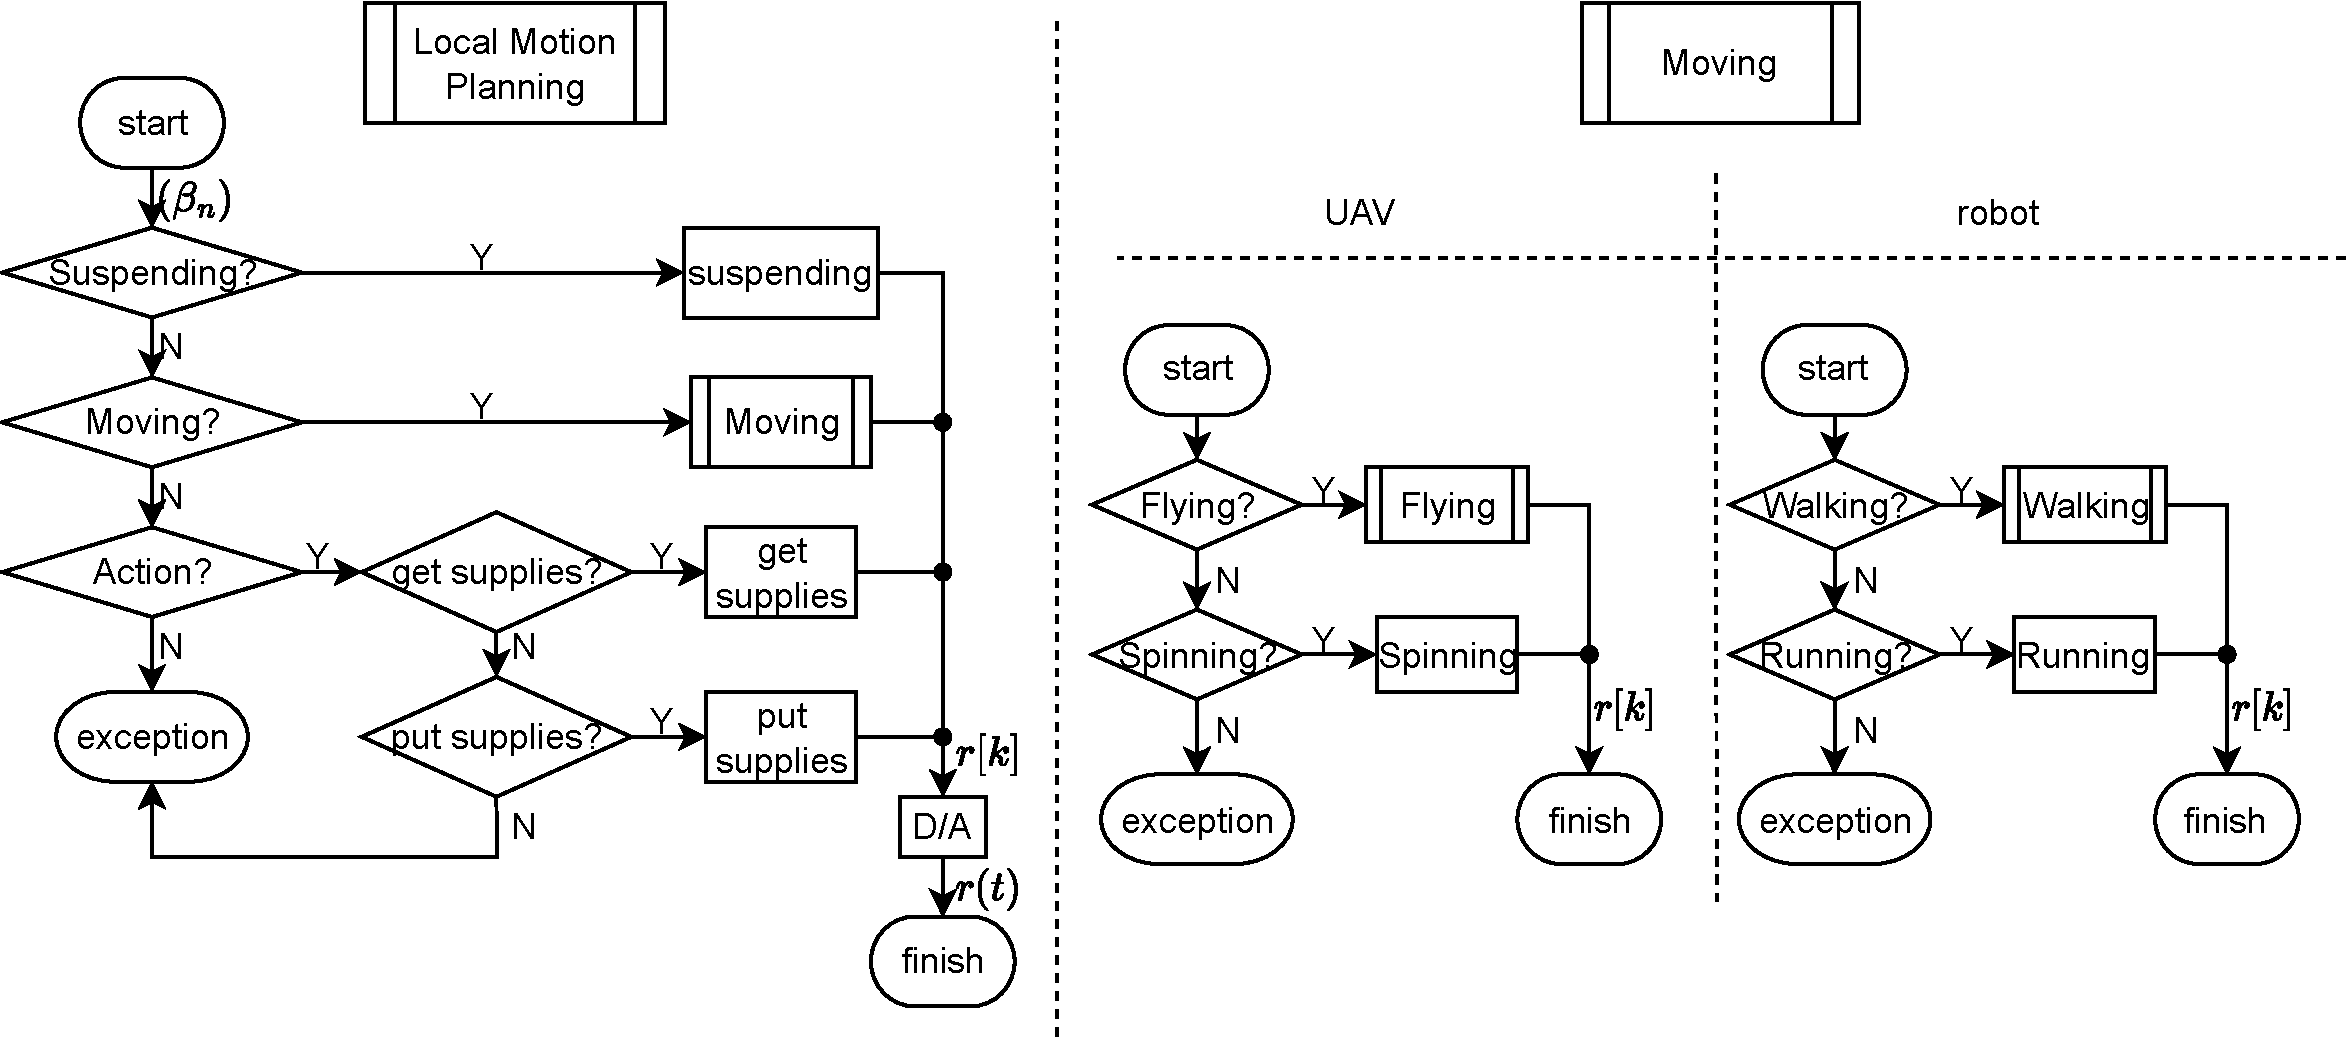
\includegraphics[scale=.12]{fig/LMP.png}\caption{The flowchart of local motion planning. The corresponding motion planning will be executed according to the behavior determined by the behavior layer. The exception terminator in figure represents an exceptional condition that performs unconsidered behaviors. The reference path $r[k]$ is a sequence (or say a discrete signal) designed by a specific behavior block.}
    \label{fig:LocalMotionPlanning}
\end{figure*}

In Fig. \ref{fig:LocalMotionPlanning}, some basic behaviors of UAV and robot mentioned before are added to illustrate the flow of this block. To limit the scope of this article, we only focus on the motion planning of flying behavior of UAV and walking behavior of robot. They are belong to moving behavior in Fig. \ref{fig:LocalMotionPlanning}. A more detailed description will be given in the next section.

\subsection{Tracking Control}
To analysis the control problem in the continuous time domain, $r[k]$ will first convert to a continuous signal by D/A convertor with a timescale, i.e., sampling period. By analyzing the dynamic model of each agent, a desired reference trajectory $r(t)$ is designed. $r(t)$ describes the position and orientation that need to be reached over time by a machine system governed by a dynamic equation. Note that the path and trajectory are distinguished in some literature. Different from path (e.g., $(\sigma_n)$ or $r[k]$), a trajectory $r(t)$ has considered the time in physic world. We also distinguish in this way in this article.

If each agent in hybrid URTS can track each own reference trajectory $r(t)$, then they can move in the physical world as we expect. To this end, a control method need to be design. It will be discussed detailly in Section IV. In addition, the sensing information collected by the sensors in this block is not only used for control but also sent back to the upper layer as shown in Fig. \ref{fig:sys}.

\section{system description of UAVs and biped robots in URTS}
In order to design a reference trajectory $r(t)$ for the motion of UAV and robot, their dynamic models must be given first. After the system description of UAV and robot, the motion planning of flying and walking as shown in Fig. \ref{fig:FandW} will be discussed subsequently and separately in the next two subsections.
\begin{figure*}[htbp]
    \centering
    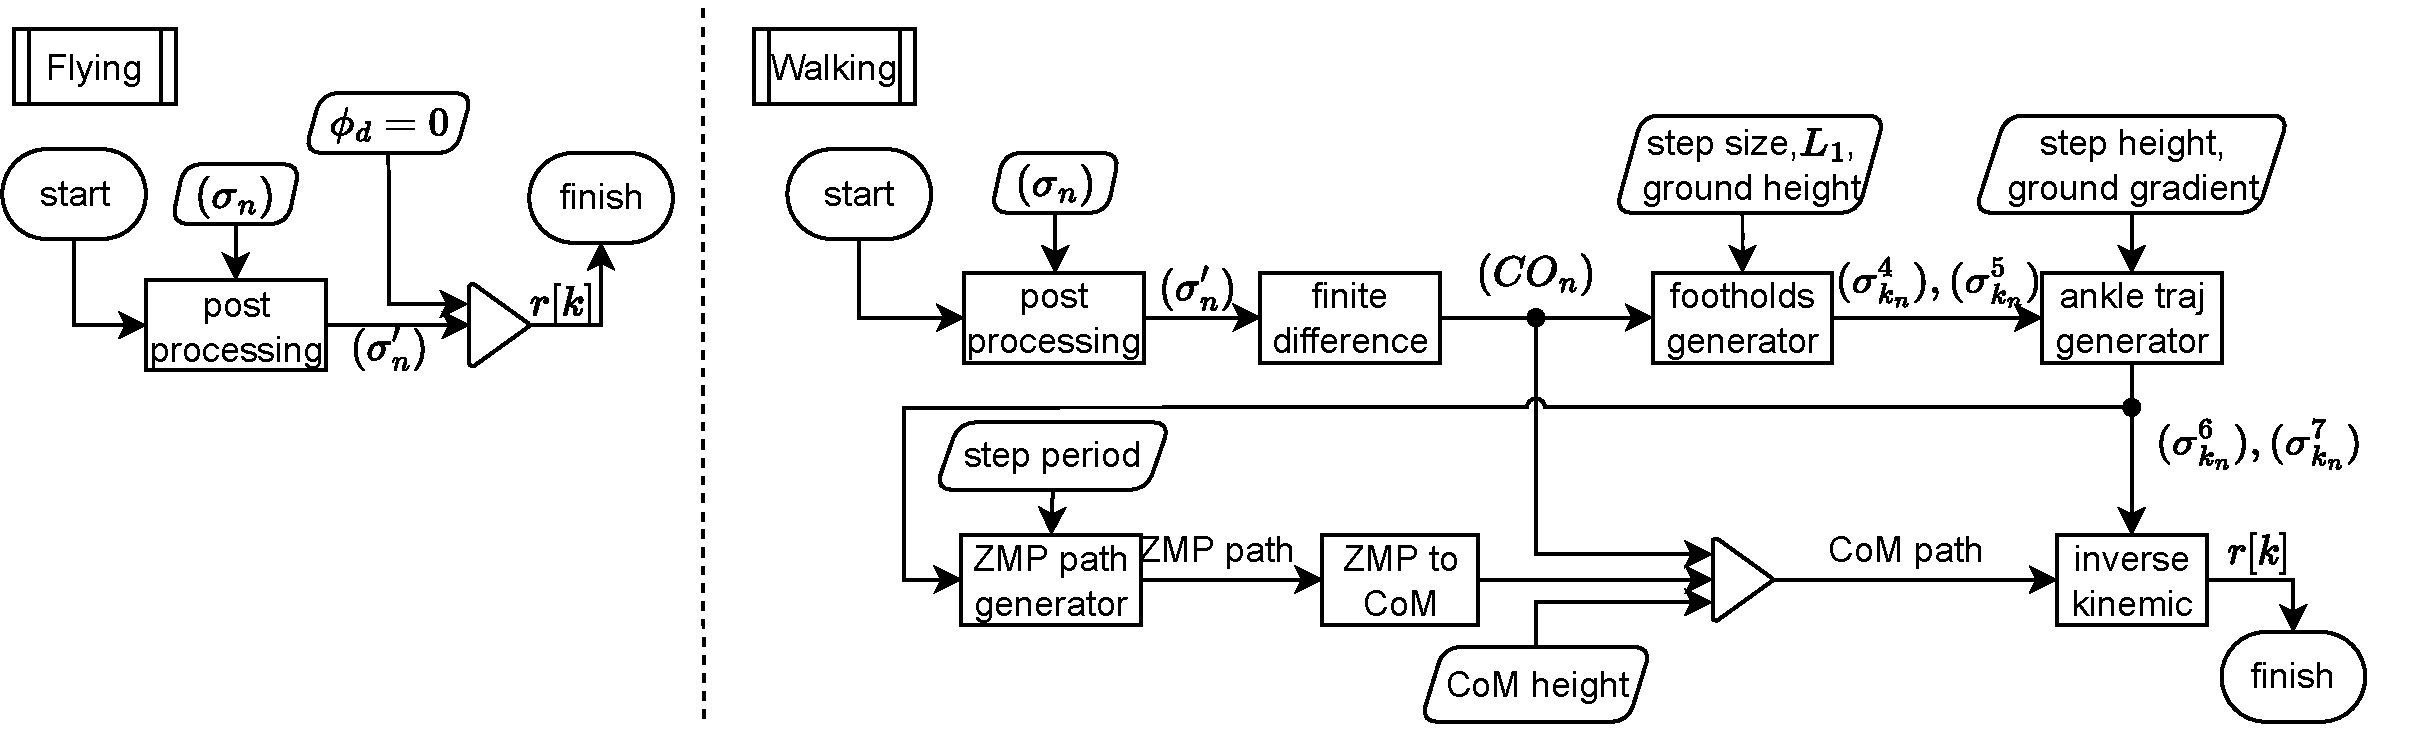
\includegraphics[scale=.12]{fig/FandW.png}\caption{The flowchart of Flying and Walking. In both blocks, a smoothed path is obtained by post-processing first. Then the respective motion of behavior is designed. The final outputs of Flying and Walking are all desired reference path $r[k]$, but its value and dimension will vary according to the dimension of the system model.}
    \label{fig:FandW}
\end{figure*}
Before the discussion of the motion planning of these two behaviors, the following assumption is maded.
\textit{
    \begin{assumption} \label{asm:cc again}
        The space between obstacles is large enough to eliminate the need for collision checking again, and the average speed of agents is slow enough to ignore dynamic constraints
    \end{assumption}
}
However, for these two behaviors, there exists an inevitable kinematic constraint on the curvature of local motion. Although an accurate reference trajectory without breaking the curvature constraint can be designed, it is not easy to solve this problem. Additionally, it is not nessasry for these two behaviors in URTS since they are uesd to move from one location to another while the effect of error during moving caused by breaking the curvature constraint is relatively insignificant. At the same time, the \textit{Assumption \ref{asm:cc again}} makes sure the error will not cause collision. As an alternative, this problem can be handled by curve fitting which can be regarded as a post-process of the path $(\sigma_n)$. The post-process will appear in the begining of motion planning process of these two behaviors as shown in Fig. \ref{fig:FandW}.

\subsection{motion planning of flying of UAV}
A dynamic model about how the UAV moves in the physical world is given first. By Newton-Euler equation, the dynamic model of UAV can be formulated as \cite{sabatino2015quadrotor}:
\begin{equation} \label{eq:uav} 
    \begin{split}
        \begin{bmatrix}
            f_u \\ \tau_u
        \end{bmatrix}&=\begin{bmatrix}
            mI & 0 \\ 0 & J
        \end{bmatrix}\begin{bmatrix}
            \ddot{X} \\ \ddot{\Theta}
        \end{bmatrix}+\begin{bmatrix}
            0 \\ \dot{\Theta}\times(J\dot{\Theta})
        \end{bmatrix}+\begin{bmatrix}
            f_g \\ 0
        \end{bmatrix}
        \\
        &+\begin{bmatrix}
            K_F & 0 \\
            0 & K_\tau
        \end{bmatrix}\begin{bmatrix}
            \dot{X} \\ \dot{\Theta}
        \end{bmatrix}
        % Form 2 of rotation matrix R(\Theta)
        % &R(\Theta)=\begin{bmatrix*}[l]
        %     \cos\theta\cos\phi & \sin\phi\sin\theta\cos\psi-\cos\phi\sin\psi & R_1 \\
        %     \cos\theta\sin\phi & R_2 & R_3 \\
        %     -\sin\theta & \sin\phi\cos\theta & R_4
        % \end{bmatrix*}
        % \\
        % &R_1=\cos\phi\sin\theta\cos\psi+\sin\phi\sin\psi
        % \\
        % &R_2=\sin\phi\sin\theta\sin\psi+\cos\phi\cos\psi
        % \\
        % &R_3=\cos\phi\sin\theta\sin\psi-\sin\phi\cos\psi
        % \\
        % &R_4=\cos\phi\cos\theta
    \end{split}
\end{equation}
where $J=\begin{bmatrix}
    J_{x} & 0 & 0 \\
    0 & J_{y} & 0 \\
    0 & 0 & J_{z}
\end{bmatrix}$, $K_F=\begin{bmatrix}
    K_{x} & 0 & 0 \\
    0 & K_{y} & 0 \\
    0 & 0 & K_{z}
\end{bmatrix}$, $K_\tau=\begin{bmatrix}
    K_{\tau_x} & 0 & 0 \\
    0 & K_{\tau_y} & 0 \\
    0 & 0 & K_{\tau_z}
\end{bmatrix}$, $f_u =\begin{bmatrix}
    f_x \\ f_y \\ f_z
\end{bmatrix} = R(\Theta)\begin{bmatrix}
    0 \\ 0 \\ F
\end{bmatrix}$, $\tau_u=\begin{bmatrix}
    \tau_x \\ \tau_y \\ \tau_z
\end{bmatrix}$, $X=\begin{bmatrix}
    x \\ y \\ z
\end{bmatrix}$, $\Theta=\begin{bmatrix}
    \phi \\ \theta \\ \psi
\end{bmatrix}$, $f_g=\begin{bmatrix}
    0 \\ 0 \\ -mg
\end{bmatrix}$, $R(\Theta)=R_z(\psi)R_y(\theta)R_x(\phi)$, $R_z(\psi)=\begin{bmatrix} % form 1
    \cos\psi & -\sin\psi & 0 \\
    \sin\psi & \cos\psi & 0 \\
    0 & 0 & 1
\end{bmatrix}$, $R_y(\theta)=\begin{bmatrix}
    \cos\theta & 0 & \sin\theta \\
    0 & 1 & 0 \\
    -\sin\theta & 0 & \cos\theta
\end{bmatrix}$, $R_x(\phi)=\begin{bmatrix}
    1 & 0 & 0 \\
    0 & \cos\phi & -\sin\phi \\
    0 & \sin\phi & \cos\phi
\end{bmatrix}$.
% where $y'$ denotes the $y$ axis after rotating the $z$ axis and $x''$ denotes the $x$ axis after rotating the $y'$ axis
$g$ is the gravity acceleration, $m$ and $J$ are the mass and inertia matrix of UAV, respectively, $\tau_u$ and $F$ are the total torque and force acting on UAV, respectively, $\Theta$ is the Euler angles in body frame, $X$ is the postion of center of mass (CoM) in inertial frame, $K_\tau$ and $K_F$ are the aerodynamic damping coefficients, and $R(\Theta)$ is the intrinsic rotation matrix from body frame to inertial frame. This model treats the UAV as a mass point and can control the force in the $z$ direction and the torque in the $x$, $y$ and $z$ direction. Hence, the reference trajectory of UAV $r(t)=[x_r(t),y_r(t),z_r(t),\phi_r(t),\theta_r(t),\psi_r(t)]^T\in\mathbb{R}^{6}$, where the subscript $r$ denotes the reference.

Now, suppose the UAV flying occurs between time step $t_1$ and $t_2$, that is, $\beta_n=\mathit{flying}, n\in\mathbb{Z}\cap[t_1,t_2]$. The corresponding path $(\sigma_n), n\in\mathbb{Z}\cap[t_1,t_2]$ will be smoothed first by linear interpolation and then by cubic spline interpolation, which gives the smoothed path $(\sigma_n'), n\in\mathbb{Z}\cap[t_1,t_1+D(t_2-t_1)], \sigma_n'\in\mathbb{R}^3$, where $D\in\mathbb{Z}^+$ is the interpolation density. Then, $(\sigma_n')$ will be the position reference path $[
    x_r[k], y_r[k], z_r[k]
]^T$. Subsequently, the orientation reference path, row angle $\phi_r[k]$, pitch angle $\theta_r[k]$ and yaw angle $\psi_r[k]$ are all considered. $\phi_r[k]$ is set to zero since no need for spinning when flying. $\theta_r[k]$ and $\psi_r[k]$ cannot be set beforehand since UAV is an underactuated system, which will be discussed in the next section. Finally, the reference path $r[k]$ of UAV can be obtained by combining them together, i.e., $r[k] = [
    x_r[k], y_r[k], z_r[k], \psi_r[k]
]^T\in\mathbb{R}^{4}$. The flowchart is shown in Fig. \ref{fig:FandW}.

% \begin{figure}[htbp]
%     \centering
%     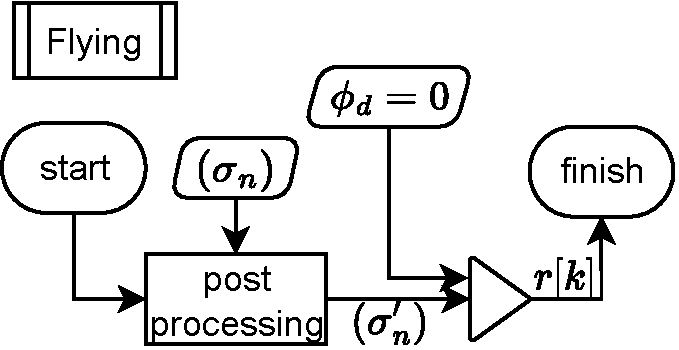
\includegraphics[scale=.5]{fig/flying.pdf}\caption{flowchart of UAV flying}%
%     \label{fig:flying}
% \end{figure}

% task space $\mathcal{T}\subset\mathbb{R}^6$.
% The terminologies, task space and joint space, are often used in reference designed in robotics. Task space is the space which the task be assigned and joint space is the space of robot joints. The forward kinematic is the mapping from joint space to task space and inverse kinematic is the inverse mapping. Since the reference of robot is in joint space ...

\subsection{motion of walking of robot}
By Lagrange equation, the dynamic model of biped robot can be formulated as:
\begin{equation} \label{eq:robot} 
    \begin{split}
        & \tau_R = M_R(q)\ddot{q} + C(q,\dot{q})\dot{q} + G(q)    
    \end{split}
\end{equation}
where $\tau_R$ is the total torque on revolute joints, $q,\dot{q},\ddot{q}\in\mathbb{R}^{12}$  are angular position, angular velocity, and angular acceleration vector of revolute joints, $M_R(q)\in\mathbb{R}^{12\times 12}$ is the inertia matrix, $C(q,\dot{q})\in\mathbb{R}^{12}$ is the Coriolis and centripetal force vector and $G(q)\in\mathbb{R}^{12}$ is the gravitational force vector. The detailed kinematic and dynamic parameters can be found in the online source \cite{ourrobot}. For robot, the reference trajectory $r(t)=q_r(t)\in\mathbb{R}^{12}$ is in the joint space. Furthermore, the walking of biped robot suffers from the falling problem, i.e, how to find a stable walking pattern to prevent robot from falling. These make the design of walking motion more difficult. In this paper, a three-dimensional linear inverted pendulum Model (3D-LIPM) \cite{kajita2001real} is used to design the walking motion.

With 3D-LIPM, we can significantly reduce the amount of computation. Let us define the body frame of robot as $\{ \widehat{X_b}, \widehat{Y_b}, \widehat{Z_b} \}$ as in \cite{ourrobot}. Taking the forward direction of robot as $\widehat{X_b}$ direction, the left direction as $\widehat{Y_b}$ direction, and the torso direction as $\widehat{Z_b}$ direction in body frame, "Falling" means the moments on the robot in $\widehat{X_b}$ and $\widehat{Y_b}$ direction are not zero. More accuately, the robot will not fall if the zero moment point (ZMP) lies in the support polygon, i.e., the convex hull of face of supported foots. The ZMP in $\widehat{X_b}$ direction can be discribed as \cite{huang2001planning} (The ZMP in $\widehat{Y_b}$ direction as the same form):
\begin{equation} \label{eq:x_zmp}
    x_{zmp} = \frac{\sum_{i=1}^{12} (m_i(\ddot{z}_i+g)x_i - m_i\ddot{x}_iz_i - I_{iy}\ddot{\Omega}_{iy})}
                   {\sum_{i=1}^{12} m_i(\ddot{z}_i+g)}
\end{equation}
where $m_i$ is the CoM, $x_i, z_i$ are the linear position components, $I_{iy}$ is the inertial component, and $\ddot{\Omega}_{iy}$ is the angular velocity component of link $i$. However, it is difficult to directly calculate the analytical solution of $q_r(t)$ through (\ref{eq:x_zmp}). Since there is a complex coordinate transformation between $q_r(t)$ and $x_i, z_i, \ddot{\Omega}_{iy}$. At the same time, it is necessary to ensure that $x_{zmp}$ falls on the support polygon but the support polygon also has a relationship with $q_r(t)$. To simplify this complex problem, an approximate solution can be derived through 3D-LIPM. It is to find CoM reference first and then obtain $q_r(t)$ by using inverse kinematic (IK) with given step size, step height, step period and CoM height. Many researchers have used this method to avoid complex calculations for ZMP of actual robot dynamic model. Although there exist a model error between the actual dynamic model and 3D-LIPM, the design process will be more simple. The overall process is shown in Fig. \ref{fig:FandW}.
% \begin{figure}[htbp]
%     \centering
%     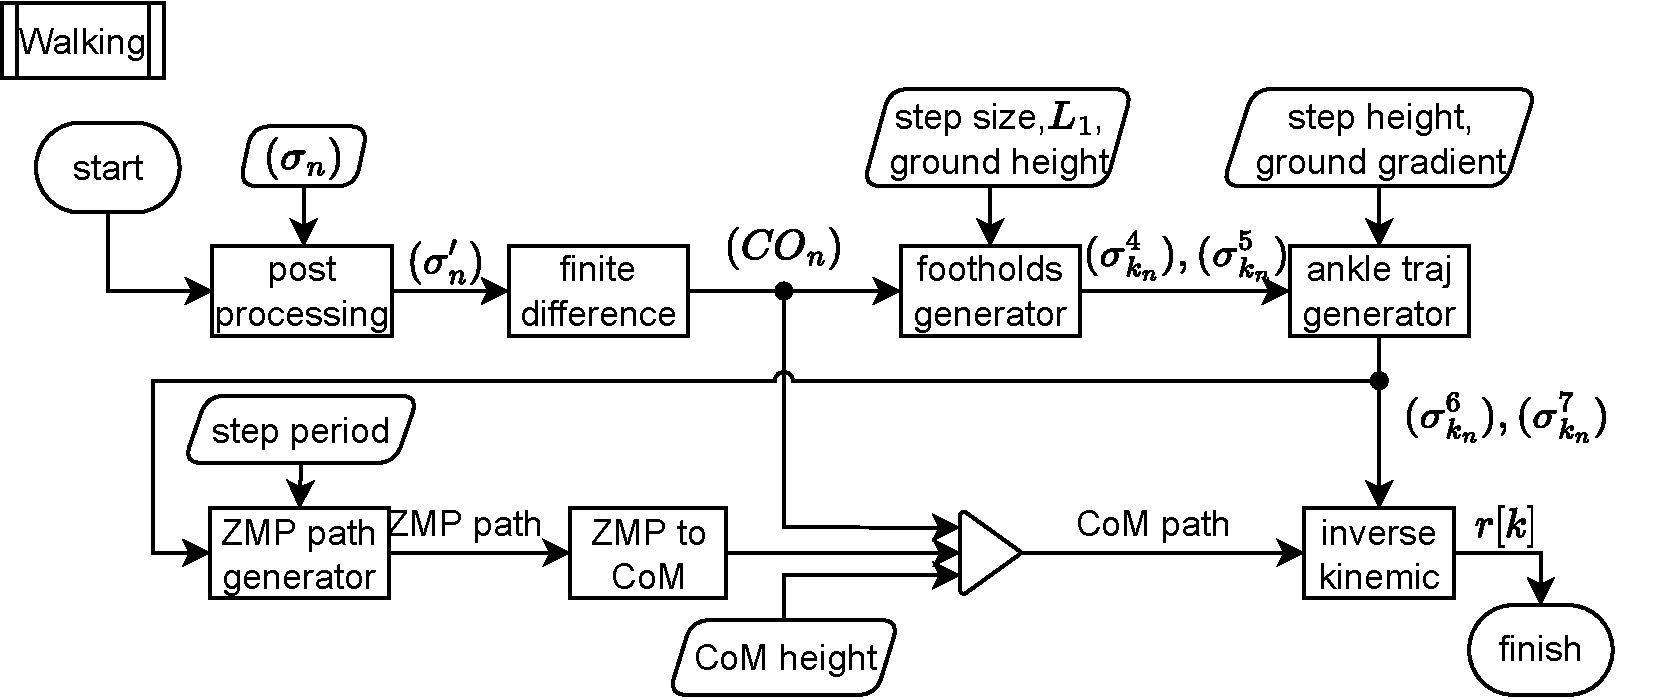
\includegraphics[scale=.3]{fig/walking.pdf}\caption{flowchart of biped robot walking}%
%     \label{fig:walking}
% \end{figure}

Following the same step in UAV, the smoothed path $(\sigma_n')$ for robot can be obtained at first. For the convenience of explanation, suppose walking is occured between time step $1$ and $N$, i.e., $n\in\mathbb{Z}\cap[1,N]$. Note that $(\sigma_n')$ is not actual CoM reference in robot case since CoM of robot need to "swinging" for balance. Despite that, $(\sigma_n')$ tells the robot the position to go so the $\widehat{X_b}$ direction can be obtained by doing finite difference on $(\sigma_n')$ due to the expectation that the robot will move forward (rather than sideways or backward). To keep torso upright, the $\widehat{Z_b}$ direction is equal to the $z$-axis in the inertial frame $\widehat{Z_g}$. Given $\widehat{X_b}$ and $\widehat{Z_b}$, $\widehat{Y_b}$ can be obtained obviously through cross product. The sequence of body frame, i.e., CoM orientation path $(CO_n)$ can be obtained through the above steps.

\textit{
    \begin{remark}
        A frame in $\mathbb{R}^3$ can be determined by giving the "position" and "orientation" with respect to a reference frame. That is, given the position and orientation of two joints in a link with known kinematics, the position and orientation of joints between them can be found by IK. Hence, we need to find the  position path and orientation path, which compose the desired path.
    \end{remark}
}

Let us denote the $x$ and $y$ component of $\sigma_n'$ in $(\sigma_n')$ as the sequence $(\sigma^{1}_{n}), \sigma^{1}_{n}\in\mathbb{R}^2$. The left and right "envelopes", $(\sigma^{2}_{n})$ and $(\sigma^{3}_{n})$, of $(\sigma^{1}_{n})$ with a fixed distance $L_1$ can be found by $(\sigma^{1}_{n})$ and $(CO_n)$ through the geometric relation between $(\sigma^{i}_{n}), i=1,2,3$, where $L_1$ is feet width (or shoulder width). Then the $x$ and $y$ component of left and right foothold paths, $(\sigma^{2}_{k_n})$ and $(\sigma^{3}_{k_n})$, can be obtained by a given step size, which are the subsequence of $(\sigma^{2}_{n})$ and $(\sigma^{3}_{n})$, respectively. Finally, left and right foothold paths $(\sigma^{i}_{k_n}), \sigma^{i}_{k_n}\in\mathbb{R}^3, i=4,5$ are found by adding $z$ component which is given by ground height.

After foothold paths are obtained, ankle position path can also be obtained by the given step height which is customized by the designer or based on the height of the obstacle to be crossed. Taking the left foothold path as an example, $x$ and $y$ component of the highest position of ankle during stride are set as middle point of two footholds $\sigma^{2}_{k_m}$ and $\sigma^{2}_{k_{m+1}}$ where $m\in\mathbb{Z}\cap[1,N-1]$, and the $z$ component is given by step height. By using cubic spline interpolation, we have the left and right ankle position paths, $(\sigma^{6}_{n})$ and $(\sigma^{7}_{n})$. The ankle orientation path is found by the gradient of ground. Finally, the left and right ankle paths, $(\sigma^{8}_{n})$ and $(\sigma^{9}_{n})$, are found by combining the position and orientation path together. So far, the remaining work is to find out the CoM path and then to combine with the ankle path to calculate the joint path through IK.

To obtain CoM postion path $(CP_n)$, ZMP path needs to be obtained first. ZMP path can be obtained through foothold paths $(\sigma^{4}_{k_n})$ and $(\sigma^{5}_{k_n})$ since ZMP needs to lie in the support face and the foothold path points out when the feet are on the ground. Suppose the CoM height $z_c$ of robot is constant when walking, then the robot model can be regarded as an 3D-LIPM:
\begin{equation} \label{eq:LIPM}
    \begin{split}
        & \ddot{x}_c = \frac{g}{z_c}(x_c - p_x) \\
        & \ddot{y}_c = \frac{g}{z_c}(y_c - p_y)
    \end{split}
\end{equation}
where $(x_c, y_c, z_c)$ is the position of CoM of the inverted pendulum, $g$ is the gravity acceleration, and $(p_x,p_y)$ is the position of ZMP on the $x$-$y$ plane. Since $z_c$, $g$ and $(p_x,p_y)$ are given, $(x_c, y_c)$ can be solved. Observing the dynamic equations in the $x$ and $y$ directions in (\ref{eq:LIPM}), it can be found that they are decoupled and thus can be calculated separately. Therefore, only the solution in the $x$ direction is given below (the $y$ direction as the same). To solve it, a method is proposed to convert it to a servo problem \cite{1241826}:
\begin{equation} \label{eq:output tracking}
    \begin{split}
        & \dot{\bar{x}}_c = A\bar{x}_c + Bu \\
        & p_x = C\bar{x}_c
    \end{split}
\end{equation}
where $\bar{x}_c = \begin{bmatrix}
    x_c \\ \dot{x}_c \\ \ddot{x}_c
\end{bmatrix}$, $A = \begin{bmatrix}
    0 & 1 & 0 \\ 0 & 0 & 1 \\ 0 & 0 & 0
\end{bmatrix}$, $B = \begin{bmatrix}
    0 \\ 0 \\ 1
\end{bmatrix}$, and $C = \begin{bmatrix}
    1 & 0 & -z_c/g
\end{bmatrix}$. Our goal is to find a control input $u$ in order that the output $p_x$ can track a ZMP reference trajectory so that the solution $x_c$ of ODE in (\ref{eq:LIPM}) can be obtained, i.e., the CoM position path is found. Unlike conventional methods, the problem is solved by the optimal control. The system is discretized first and the discrete LQ tracker is employed to achieve the output tracking. The formulation can be found in TABLE 4.4-1 in \cite{lewis2012optimal}. The CoM position path $(CP_n)$ then be obtained by combining $x_c$ and $y_c$ with $z_c$.

By combining the CoM orientation path $(CO_n)$ and position path $(CP_n)$, CoM path can be obtained. Finally, the joint path, i.e., reference path $r[k]\in\mathbb{R}^{12}$ of robot can be found by solving IK.

\section{Tracking control of each agent in hybrid URTS}
Before converting $r[k]$ to $r(t)$, we first convert the UAV dynamic system in (\ref{eq:uav}) and robot dynamic system in (\ref{eq:robot}) into a form called agent dynamic model to analyze their tracking control problems together. Through some appropriate variable transformations, we have:
\begin{equation} \label{eq:agent} 
    M(x(t))\ddot{x}(t) + H(x(t),\dot{x}(t)) = u(t)
\end{equation}
where $u(t)\in\mathbb{R}^n$ is the control input vector, $x(t)\in\mathbb{R}^n$ is state vector, $M(x(t))\in\mathbb{R}^{n\times n}$ is inertia matrix, and $H(x(t),\dot{x}(t))\in\mathbb{R}^n$ is non-inertial force vector. The control law is given as:
\begin{equation} \label{eq:control}
    u(t)= M(r(t))(\ddot{r}(t) + u_{fb}(t)) + H(r(t),\dot{r}(t)) 
\end{equation}
where $r(t)\in\mathbb{R}^n$ is the desired reference trajectory, $M(r(t)), \ddot{r}(t)\mathbin{,} H(r(t), \dot{r}(t))$ are the feedfoward control terms for canceling system nonlinearity, and $u_{fb}(t)$ is the feedback control law to be futher designed for improving system robustness. For UAVs, we have $u(t)=\begin{bmatrix}
    f_u \\ \tau_u
\end{bmatrix}$, $x(t)=\begin{bmatrix}
    X \\ \Theta
\end{bmatrix}$, $M(x(t))=\begin{bmatrix}
    mI & 0 \\ 0 & J
\end{bmatrix}$, $H(x(t),\dot{x}(t))=\begin{bmatrix}
    0 \\ \dot{\Theta}\times(J\dot{\Theta})
\end{bmatrix}+\begin{bmatrix}
    f_g \\ 0
\end{bmatrix}+\begin{bmatrix}
    K_F & 0 \\
    0 & K_\tau
\end{bmatrix}\begin{bmatrix}
    \dot{X} \\ \dot{\Theta}
\end{bmatrix}$, and $n=6$ by (\ref{eq:uav}). For robots, we have $u(t)=\tau_R$, $x(t)=q$, $M(x(t))=M_R(q)$, $H(x(t),\dot{x}(t))=C(q,\dot{q})\dot{q} + G(q)$, and $n=12$ by (\ref{eq:robot}).

To complete the design of reference trajectory $r(t)$ of each agent, a D/A converter is used to transform the reference path $r[k]$ (output of local motion planning) into a continuous signal $r'(t)$ as shown in Fig. \ref{fig:tracking}. For UAV, we get $r'(t) = [x_r, y_r, z_r, \psi_r]^T\in\mathbb{R}^{4}$. Besides, it can be seen that the control input $u(t)=[f_x, f_y, f_z, \tau_x, \tau_y, \tau_z]^T\in\mathbb{R}^6$ we design of UAV (\ref{eq:control}) is different from the actual control input for actuator $u'(t)=[F, \tau_x, \tau_y, \tau_z]^T\in\mathbb{R}^4$ of UAV since UAV is an underactuated system. The two degrees of freedom we reserved in Section III-A, i.e., $\phi_r$ and $\theta_r$, are just to solve this problem. By substituting $\Theta=\begin{bmatrix}
    \phi_r \\ \theta_r \\ \psi_r
\end{bmatrix}$ into $\begin{bmatrix}
        f_x \\ f_y \\ f_z
\end{bmatrix} = R(\Theta)\begin{bmatrix}
        0 \\ 0 \\ F
\end{bmatrix} $ from UAV dynacmis (\ref{eq:uav}), the 3 unknown variables $F$, $\phi_r$ and $\theta_r$ can be found from these 3 equations using inverse dynamic because $f_x$, $f_y$, $f_z$ and $\psi_r$ are given. Combining $\phi_r$ and $\theta_r$ with $r'(t)$, we obtain $r(t)= [x_r, y_r, z_r, \phi_r, \theta_r, \psi_r]$. For robot, we get $r'(t)=r(t)\in\mathbb{R}^{12}$ and $u'(t)=u(t)\in\mathbb{R}^{12}$ since robot is a fully actuated system. So far, the design of reference trajectory $r(t)$ of each agent is done. The flowchart can be found in the reference generator block in Fig. \ref{fig:tracking}.
\begin{figure*}[htbp]
    \centering
    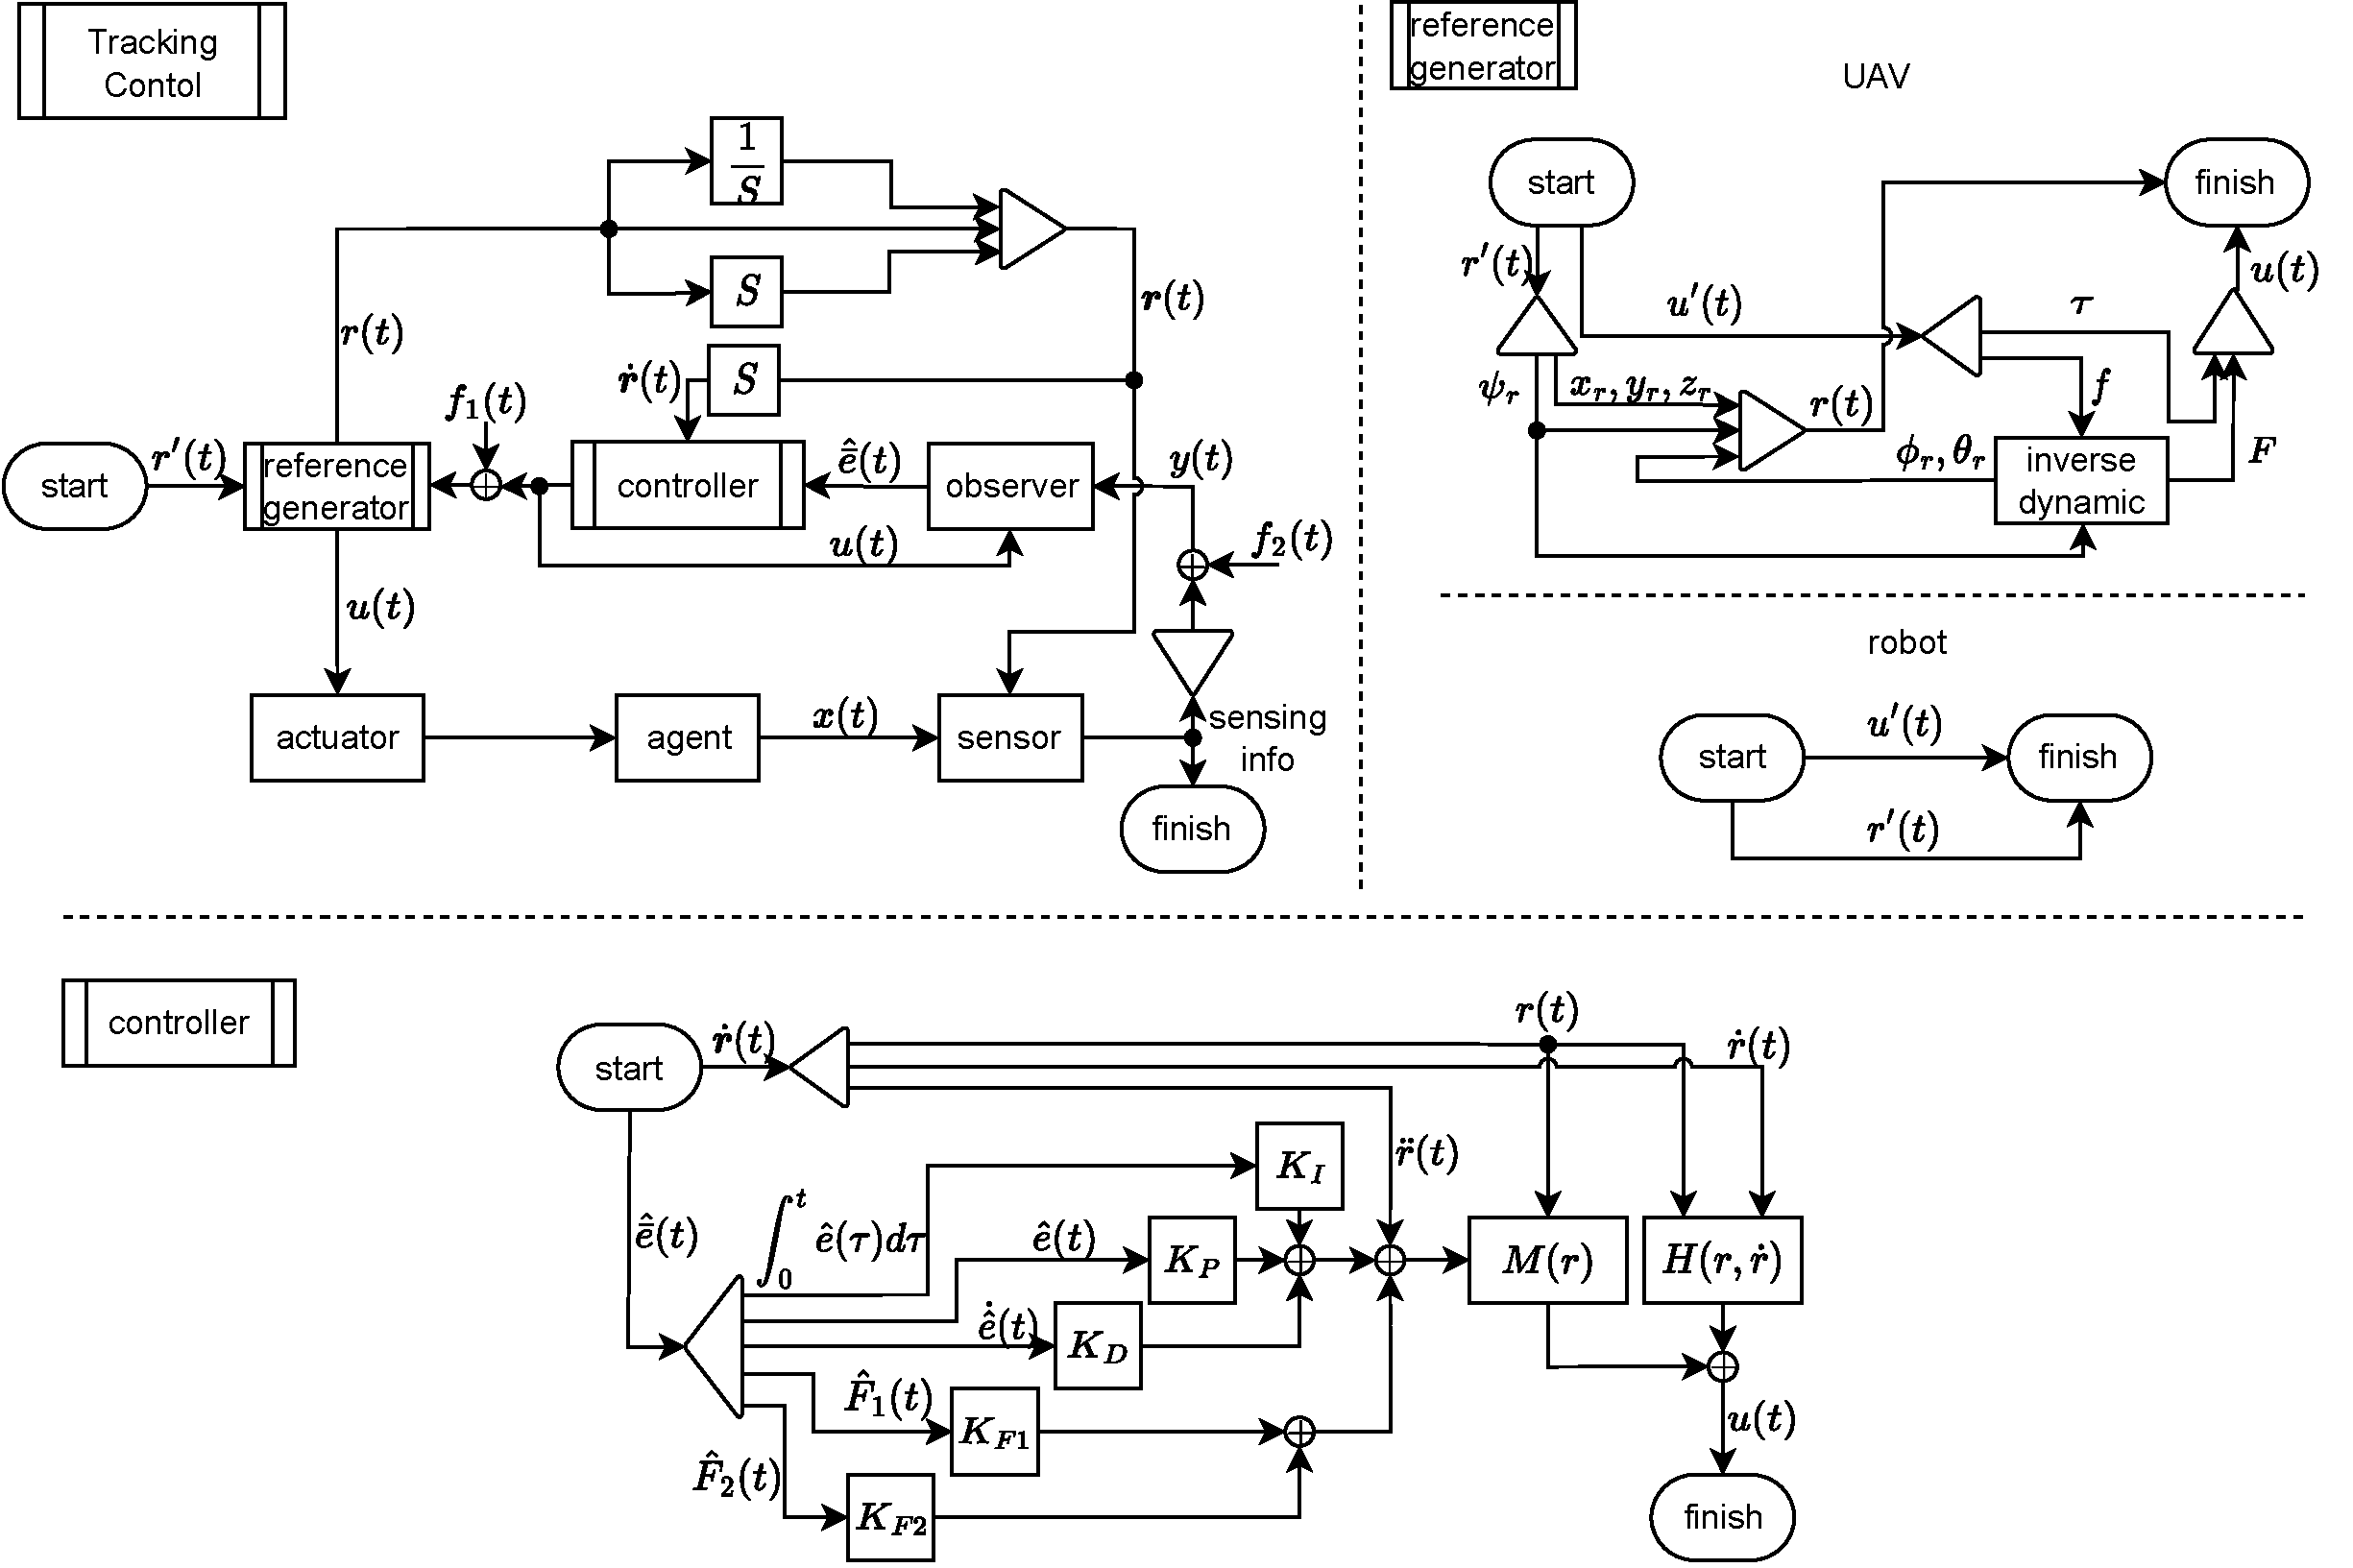
\includegraphics[scale=.12]{fig/tracking.png}\caption{The flowchart of tracking control in the hybrid URTS. The control scheme of UAV and robot in URTS is only different from the reference generator block. The reason is that the underactuated nature of the UAV imposes the limitation on the control input and reference trajectory. By introducing this block, a general $H_\infty$ decentralized observer-based feedforward-linearized PID FTC for an agent in URTS is proposed.}
    \label{fig:tracking}
\end{figure*}

\textit{
    \begin{remark}
        Let $r_{i,j}(t)$ be the reference trajectory $r(t)$, $r_{i,j}[k]$ be the reference path $r[k]$, $(\beta_n)_{i,j}$ be the behavior sequence $(\beta_n)$, $(\sigma_n)_{i,j}$ be the collision-free path $(\sigma_n)$, $q_{start,i,j}$ be the current configuration $q_{start}$, and $q_{goal,i,j}$ be the goal configuration $q_{goal}$ of the agent $\alpha_{i,j}$ in the hybrid URTS. As long as $\alpha_{i,j}$ can track $r_{i,j}(t)$, the URTS works as we expect since the previous blocks, i.e, task allocation, path planning, behavior layer and local motion planning, have completed their respective responsibilities and found the corresponding values $q_{start,i,j}$, $q_{goal,i,j}$, $(\sigma_n)_{i,j}$, $(\beta_n)_{i,j}$ and $r_{i,j}[k]$. That is, $r_{i,j}(t)$ is the reference trajectory that can complete specific task, follow specific path and perform specific behavior.
    \end{remark}
}

To make the model more realistic, the following external disturbances encountered in actual scenarios are considered:
\begin{enumerate}
    \item For each agent, there exists coupling effect due to co-channel interference in communication between agents \cite{9834947}.
    \item For each agent, there exists cyber-attack on communication network between agents and ground station.
    \item For each agent, there exists sensor noise.
    \item For each UAV, there exists wind disturbance \cite{9075385}.
    \item For each robot, there exists ground reaction force \cite{chen2013human}. 
\end{enumerate}
Let $x_{i,j}(t), i=1,2,\dots,N_T, j=1,2,\dots,N_A$ denote the state vector of agents $\alpha_{i,j}$. The coupling disturbance $c(t)$ can be represented as \begin{equation} \label{eq:UAV couple}
    c(t) = \sum_{k = 1, k \neq i}^{N_T}D_{i, 1, k}(x_{i, 1}(t))x_{k, 1}(t)
\end{equation} for UAV $\alpha_{i, 1}$ and \begin{equation} \label{eq:robot couple}
    c(t) = \sum_{k = 1, k \neq j'}^{N_A}D_{i, j', k}(x_{i, j'}(t))x_{i, k}(t)
\end{equation} for robot $\alpha_{i, j'}$ where $j'=2,3,...,N_A$ \cite{9834947}. Since the ground station is responsible for the calculation, the calculated control command in (\ref{eq:control}) will be transmitted to the agent through the network channel in URTS. Therefore, the coupling effect due to co-channel interference and the cyber-attack signal will deteriorate the control command. In addition, the wind disturbance and the ground reaction force will apply extra force on an agent in (\ref{eq:agent}). Therefore, through appropriate conversion, the above disturbances can be equivalent to a disturbance force $c(t)$ + $d_1(t)\in\mathbb{R}^n$ where $d_1(t)$ is the non-coupling disturbance. The nominal system in (\ref{eq:agent}) of an agent then be rewrited as the following real system:
% The coupling effect for an agent \textit{$agent_{i,j}$} in URTS can be expressed as the form $\sum_{i'=1,i'\neq i}^{N_i}\sum_{j'=1,j'\neq j}^{N_j}\textit{c}_{i,j}(x_{i,j}(t))\times x_{i',j'}(t)$ where $x_{i,j}(t)$ is the own state.
\begin{equation} \label{eq:agent d1} 
    M(x(t))\ddot{x}(t) + H(x(t),\dot{x}(t)) = u(t) + c(t) + d_1(t)
\end{equation}
% \subsubsection{Internal uncertainties}
% In practice, there is uncertaintiey in the parameters of inertia matrix $M$, Coriolis and centripetal force vector $C$, gravitational force vector $G$, and friction vector $F$. Its effect can be expressed as:
% \begin{equation} \label{eq:internal}
%     \begin{split}
%         &M = M_0 + \Delta M, C = C_0 + \Delta C
%         \\
%         &G = G_0 + \Delta G, F = F_0 + \Delta F
%     \end{split}
% \end{equation}
% where $M_0, C_0, G_0$ and  $F_0$ is the nominal part and $\Delta M,\Delta C,\Delta G$ and $\Delta F$ is the uncertain part.

Now, substituting (\ref{eq:control}) into (\ref{eq:agent d1}) and subtracting $M(x(t))\ddot{r}(t)$ from the left and right sides, we have:
\begin{equation} \label{eq:agent1}
    \begin{split}
        & M(x(t))(\ddot{x}(t)-\ddot{r}(t)) + H(x(t),\dot{x}(t)) \\
        & =(M(r(t))-M(x(t)))\ddot{r}(t) + M(r(t))u_{fb}(t) \\
        & + H(r(t),\dot{r}(t)) + c(t) + d_1(t)
    \end{split}
\end{equation}
By Multipling $M(x(t))^{-1}$ from the left and right sides and with some arrangments, we have:
\begin{equation} \label{eq:error, state eq}
    \ddot{e}(t) = u_{fb}(t) + f_1(t)
\end{equation}
where $f_1(t) = M(x(t))^{-1}(-\Delta M (\ddot{r}(t)+u_{fb}(t)) -\Delta H + c(t) + d_1(t))\in\mathbb{R}^n$ is considered as the actuator fault signal, $\Delta M \triangleq M(x(t)) - M(r(t))$ and $ \Delta H \triangleq H(x(t),\dot{x}(t)) - H(r(t),\dot{r}(t))$ are the error terms from feedforward compensation, and $e(t)= x(t)-r(t)$ is the tracking error.
% \textit{
%     \begin{remark}
%         Although the error terms $\Delta e$, $\Delta M$ and $\Delta H$ caused by the difference between state $x(t)$ and estimated state $\hat{x}(t)$ are not necessarily bounded, they can still be estimated as long as they are smooth.
%     \end{remark}
% }
Let $\pmb{e}(t)=\begin{bmatrix}
    \int_{0}^{t}e^T(\tau)d\tau & e^T(t) & \dot{e}^T(t)
\end{bmatrix}^T\in\mathbb{R}^{3n}$, (\ref{eq:error, state eq}) can be rewrited as:
\begin{equation} \label{eq:linear f1}
    \dot{\pmb{e}}(t)=A\pmb{e}(t)+B(u_{fb}(t)+f_1(t))
\end{equation}
where $ A = A_0\otimes I_n, B = B_0\otimes I_n$
with $A_0 = \begin{bmatrix}
    0 & 1 & 0 \\ 0 & 0 & 1 \\ 0 & 0 & 0
\end{bmatrix}, B_0 = \begin{bmatrix}
0 \\ 0 \\ 1
\end{bmatrix}$. 

Through above analysis, the tracking control problem of the nonlinear system with external disturbance (\ref{eq:agent d1}) is transformed into the regulation problem of the linear system (\ref{eq:linear f1}) with fault signal by the feedforward linearization. The remaining step is to design an appropriate feedback control law $u_{fb}(t)$ to make the linear system stable. In a real system, the feedback information is measured by sensor, i.e, the state $x(t)$ in (\ref{eq:agent}) is unavailable. At the same time, the sensor fault on sensor also need to be considered as mentioned before. Since the sensor information will transmitted back to the ground station for calculating control command through the network channel in URTS, not only the sensor noise but the cyber-attack signal are concerned. Let $\pmb{x}(t)=\begin{bmatrix}
    \int_{0}^{t}x^T(\tau)d\tau & x^T(t) & \dot{x}^T(t)
\end{bmatrix}^T$
% Suppose the total effect can be equivalent to an unknown sensor fault signal $f_2(t)\in \mathbb{R}^{n}$ with same size as $f_1(t)$, 
, the measurement output equation can be described as:
\begin{equation} \label{eq:agent output}
    y(t) = C\pmb{x}(t) + B_2f_2(t)
\end{equation}
where $y(t)\in\mathbb{R}^{l}$ is the output vector, $C\in\mathbb{R}^{l\times 3n}$ is the output matrix, $B_2\in\mathbb{R}^{l\times o}$ is the input matrix of sensor fault signal $f_2(t)\in\mathbb{R}^o$. Let us define $\pmb{r}(t)=\begin{bmatrix}
    \int_{0}^{t}r^T(\tau)d\tau & r^T(t) & \dot{r}^T(t)
\end{bmatrix}^T$ to modify the output equation (\ref{eq:agent output}) and combine it with (\ref{eq:linear f1}), we have the following tracking error dynamic system of an agent in the hybrid URTS:
\begin{equation} \label{eq:error}
    \begin{split}
        & \dot{\pmb{e}}(t)=A\pmb{e}(t)+B(u_{fb}(t)+f_1(t)) \\
        & y(t) = C\pmb{e}(t) + C\pmb{r}(t) + B_2f_2(t)   
    \end{split}  
\end{equation}
% where $f_i(t)\in \mathbb{R}^{n_i}, i=1,2$ with $n_1=n$ and $n_2 = n$.

To deal with the fault signals $f_i(t),i=1,2$, a smoothing signal model is introduced \cite{9306757}:
%% teacher say the following assumption too strong
% First, we need a model of the fault signal. In general, constructing a model for an unknown signal is impossible since there is no information about it. Hence, the following assumption is maded:
% \begin{assumption} \label{asm:smooth}
%     The first $p-1$ derivatives of the fault signals $f_i(t), i=1,2$ all exist and are continuous, i.e., $f_i(t)\in C^{p-1}$.
% \end{assumption}
% Under the assumption, now we can construct a smoothing signal model by finite difference method. To obtain a state-space representation, the derivative of the fault signals $\dot{f}_i(t)$ with uniform grid $h$ are needed, which can be expressed as:
% \begin{equation} \label{eq:df}
%     \dot{f}_i(t)=\sum_{k\in{Z_0}}\frac{a_k f_i(t-kh)}{h} + R_{p-1}(t), Z_0\subset\mathbb{Z}
% \end{equation}
% where $R_{p-1}(t)\in O(h^{p-1})$ denotes the remainder term, and $p=\vert{Z_0}\vert > 1$ is the accuracy of difference. The derivative of $f_i(t-kh),k\in{Z_0}$ in (\ref{eq:df}) is also needed. For the convenience of analysis, let us choose $Z_0=\{ 0,1,\dots,p-1 \}$. By changing index $k$ to $j$, the derivative of $f_i(t-jh),j\in{Z_0}$ can be obtained by (\ref{eq:df}):
% \begin{equation} \label{eq:df1}
%     \dot{f}_i(t-jh)=\sum_{k=0}^{p-1}\frac{a_{j,k} f_i(t-kh)}{h}+\epsilon_j(t)
% \end{equation}
% where $\epsilon_j(t)\in O(h^{p-1})$. By arranging $\dot{f}_i(t-jh)$ into a state-space representation, we have:
%
% where $F_i(t)=\begin{bmatrix}
%     f_i^T(t) & f_i^T(t-h) & \dots & f_i^T(t-kh)
% \end{bmatrix}^T$, $v_i(t)=\begin{bmatrix}
%     \epsilon_0^T(t) & \epsilon_1^T(t) & \dots & \epsilon_{p-1}^T(t)
% \end{bmatrix}^T$, and $A_i=[a_{j,k}]\otimes I_{n}$. 
% Then, the fault signals $f_i(t), i=1,2$ are the output of the system in (\ref{eq:smooth model})
% \begin{equation} \label{eq:8}
%     f_i(t)=C_iF_i(t)
% \end{equation}
% where $C_i=\begin{bmatrix}
%     1 & 0 & \dots & 0
% \end{bmatrix}\otimes I_{n}$.
\begin{equation} \label{eq:smooth model}
    \begin{split}
        & \dot{F}_i(t)=A_iF_i(t)+v_i(t) \\
        & f_i(t)=C_iF_i(t)        
    \end{split}
\end{equation}
where $F_i(t)=\begin{bmatrix}
    f_i^T(t) & f_i^T(t-h) & \dots & f_i^T(t-wh)
\end{bmatrix}^T\in\mathbb{R}^{(w_i+1)n_i}$, $A_i\in\mathbb{R}^{{(w_i+1)n_i}\times{(w_i+1)n_i}}$, $v_i(t)$ is the model error, $C_i=\begin{bmatrix}
        1 & 0 & \dots & 0
    \end{bmatrix}\otimes I_{n_i}$, and $w_i$ is the window size of smoothing signal model with $n_1=n$ and $n_2 = o$. Substituting (\ref{eq:smooth model}) into (\ref{eq:error}), we get the following augmented tracking error system of an agent:
\begin{equation} \label{eq:e_bar}
    \begin{split}
        & \dot{\bar{e}}(t) = \bar{A}\bar{e}(t)+\bar{B}u_{fb}(t)+\bar{v}(t) \\
        & y(t)=\bar{C}\bar{e}(t) + C\pmb{r}(t)
    \end{split}
\end{equation}
where $\bar{e}(t) = \begin{bmatrix}
    \pmb{e}(t) \\ F_1(t) \\ F_2(t)
\end{bmatrix}$ is the augmented tracking error, $\bar{A}=\begin{bmatrix}
    A & BC_1 & 0 \\
    0 & A_1 & 0 \\
    0 & 0 & A_2
\end{bmatrix}$, $\bar{B}=\begin{bmatrix}
    B \\ 0 \\ 0
\end{bmatrix}$, $\bar{C}=\begin{bmatrix}
    C & 0 & B_2C_2
\end{bmatrix}$, and $\bar{v}(t)=\begin{bmatrix}
    0 \\ v_1(t) \\ v_2(t)
\end{bmatrix}$.
% \textit{
%     \begin{remark}
%         The equation (\ref{eq:df}) is derived by Taylor expansion, so Assumption \ref{asm:smooth} is nessasry. Unlike previous work, a finite-difference-method-based modeling method is proposed, which reduce the approximation error between origin fault signal and its smooth model. Besides, the fault signals $f_i(t)$ are assumed to be of differentiability class $C^{p-1}$ rather than bounded, which will make the proposed method more general for practical scenario.
%     \end{remark}
% }
Since the fault signals become a state variable of the augmented tracking error system of an agent in (\ref{eq:e_bar}), their corruption on the tracking error dynamic system in (\ref{eq:error}) can be avoided. A Luenberger observer is proposed to estimate them and origin state simutaniously to achieve active FTC by the following estimation system:
\begin{equation} \label{eq:e_hat}
    \begin{split}
        & \dot{\hat{\bar{e}}}(t)=\bar{A}\hat{\bar{e}}(t)+\bar{B}u_{fb}(t)-{L}(y(t)-\hat{y}(t)) \\
        & \hat{y}(t)=\bar{C}\hat{\bar{e}}(t) + C\pmb{r}(t)
    \end{split}
\end{equation}
\begin{assumption}
    The augmented tracking error system (\ref{eq:e_bar}) of an agent is observable, i.e., $rank\begin{bmatrix}
        zI-\bar{A} \\ \bar{C}
    \end{bmatrix} = 3n + (w_1+1)n + (w_2+1)o, \forall z \in eig(\bar{A})$.
\end{assumption}
The robust PID FTC law of each agent is given as:
\begin{equation} \label{eq:u_fb}
    u_{fb}(t)=K\hat{\bar{e}}(t)
\end{equation}
where $K = \begin{bmatrix}
    K_I & K_P & K_D & K_{F_1} & K_{F_2}
\end{bmatrix}$ is the total control gain, $K_P,K_I,K_D$ are the PID control gain for position tracking error $e(t)$, and $K_{F_i}, i=1,2$ are the fault control gain. Let us define the augmented estimation error $\tilde{e}(t)=\bar{e}(t)-\hat{\bar{e}}(t)$, the augmented estimation error system can be obtained by (\ref{eq:e_bar}) and (\ref{eq:e_hat}):
\begin{equation} \label{eq:e_tilde}
    \dot{\tilde{e}}(t) = \bar{A}\tilde{e}(t) +L\bar{C}\tilde{e}(t)
\end{equation}
Combining (\ref{eq:e_bar}), (\ref{eq:u_fb}), and (\ref{eq:e_tilde}), we have the following augmented tracking and estimation error system of each agent in the hybrid URTS:
\begin{equation} \label{eq:x_tilde}
    \dot{\tilde{x}}(t) = \tilde{A}\tilde{x}(t)+\tilde{v}(t)
\end{equation}
where $\tilde{x}(t)=\begin{bmatrix}
    \bar{e}(t) \\ \tilde{e}(t)
\end{bmatrix}$, $\tilde{A}=\begin{bmatrix}
    \bar{A}+\bar{B}K & -\bar{B}K \\ 0 & \bar{A}+L\bar{C}
\end{bmatrix}$, and $\tilde{v}(t)=\begin{bmatrix}
    \bar{v}(t) \\ \bar{v}(t)
\end{bmatrix}$

In order to enable the designed control gain $K$ in (\ref{eq:u_fb}) and observer gain $L$ in (\ref{eq:e_hat}) to achieve a specific performance for the augmented system in (\ref{eq:x_tilde}) under the disturbance $\bar{v}(t)$, the robust $H_\infty$ decentralized observer-based tracking control strategy below a prescribed disturbance attenuation level $\rho^2$ for each agent in hybrid URTS is given as:
\begin{equation} \label{Hinf}
    % \begin{split}
    \resizebox{1\hsize}{!}{    
        % & H_{\infty}(K, L) \\
        % & = 
        $\frac{\int_{0}^{t_f}(\bar{e}^T(t)Q_1\bar{e}(t) + \tilde{e}^T(t)Q_2\tilde{e}(t) + u_{fb}^T(t)Ru_{fb}(t))dt - V(\tilde{x}(0))}{\int_{0}^{t_f}\tilde{v}^T(t)\tilde{v}(t)dt}\leq \rho^2$
    }
    % \end{split}
\end{equation}
where $t_f$ is the final time, $Q_1 \geq 0$ is the tracking error weighting matrix, $Q_2 \geq 0$ is the estimation error weighting matrix, $R > 0$ is the weighting matrix of control effort, $V(\tilde{x}(0))$ is the initial condition effect on the augmented system in (\ref{eq:x_tilde}), and $\tilde{v}(t)$ is the total disturbance needed to be attenuated. If we can find the control gain $K$ and observer gain $L$ such that (\ref{Hinf}) holds, then the effect of total disturbance $\tilde{v}(t)$ on augmented tracking error $\bar{e}(t)$ and augmented estimation error $\tilde{e}(t)$ can be attenuated to a prescribed level $\rho^2$ from the viewpoint of energy. Before analyzing the robust $H_\infty$ decentralized observer-based tracking control problem of each agent in (\ref{Hinf}), the following lemmas are given:
\begin{lemma}[\cite{boyd1994linear}] \label{lemma1}
    For any matriices $X$ and $Y$ with appropriate dimensions, and matrix $R=R^T>0$ the following inequality holds:
    \begin{equation} \label{}
        X^T Y + Y^T X \leq X^T R^{-1}X + Y^T R Y
    \end{equation}  
\end{lemma}
\begin{lemma}[Schur Complement\cite{boyd1994linear}] \label{lemma2}
    For the matrices $X=X^T,Y=Y^T$ and matrix $R$ with appropriate dimensions the following statement is true:
    \begin{equation} \label{}
        \begin{bmatrix}
            X & R \\ R^T & Y 
        \end{bmatrix} > 0 \Leftrightarrow Y>0, X-RY^{-1}R^T>0
    \end{equation}
\end{lemma}
Then, the following theorem is given.
\begin{theorem} \label{theorem1}
    If there exists matrices $P=P^T>0, K,L$ such that the following matrix inequality hold:
    \begin{equation} \label{BMI1}
        Q + P\tilde{A} + \tilde{A}^T P + \tilde{K}^TR\tilde{K} + \frac{1}{\rho^2}PP \leq 0
    \end{equation}
    where $\tilde{K}=\begin{bmatrix}
        K & -K
    \end{bmatrix}$, $Q=\begin{bmatrix}
        Q_1 & 0 \\ 0 & Q_2
    \end{bmatrix}$, then the $H_\infty$ decentralized observer-based tracking control strategy in (\ref{Hinf}) can be achieved.
\end{theorem}
\begin{proof}
    Choose the Lyapunov function $V(\tilde{x}(t))=\tilde{x}^T(t)P\tilde{x}(t)$ for the augmented system (\ref{eq:x_tilde}) with $P=P^T>0$, we have:
    \begin{equation} \label{pf:1}
        \begin{split}
            & \int_{0}^{t_f}(\tilde{x}^T(t)Q\tilde{x}(t) + u_{fb}^T(t)Ru_{fb}(t))dt \\
            & = V(\tilde{x}(0)) - V(\tilde{x}(t_f)) + \int_{0}^{t_f}(\tilde{x}^T(t)Q\tilde{x}(t) \\
            & + u_{fb}^T(t)Ru_{fb}(t) + \dot{V}(\tilde{x}(t)))dt \\
            & \leq V(\tilde{x}(0)) + \int_{0}^{t_f}(\tilde{x}^T(t)Q\tilde{x}(t) + \\
            & u_{fb}^T(t)Ru_{fb}(t) + Sym(\dot{\tilde{x}}^T(t)P\tilde{x}(t)))dt
        \end{split}
    \end{equation}
    By (\ref{eq:x_tilde}) and Lemma \ref{lemma1}, we have:
    \begin{equation} \label{pf:2}
        \begin{split}
            & Sym(\dot{\tilde{x}}^T(t)P\tilde{x}(t)) \\
            & = Sym((\tilde{A}\tilde{x}(t)+\tilde{v}(t))^TP\tilde{x}(t)) \\
            & = \tilde{x}^T(t)(P\tilde{A} + \tilde{A}^T P + \frac{1}{\rho^2}PP)\tilde{x}(t) + \rho^2\tilde{v}^T(t)\tilde{v}(t)
        \end{split}
    \end{equation}
    Substituting (\ref{eq:u_fb}), (\ref{pf:2}) and $\tilde{x}^T(t)Q\tilde{x}(t)=\bar{e}^T(t)Q_1\bar{e}(t)+\tilde{e}^T(t)Q_2\tilde{e}(t)$ into (\ref{pf:1}), we get:
    \begin{equation*} \label{pf:3}
        \begin{split}
            & \int_{0}^{t_f}(\bar{e}^T(t)Q_1\bar{e}(t)+\tilde{e}^T(t)Q_2\tilde{e}(t))dt + u_{fb}^T(t)Ru_{fb}(t))dt \\
            & \leq V(\tilde{x}(0)) + \int_{0}^{t_f}(\tilde{x}^T(t)(Q + P\tilde{A} + \tilde{A}^T P +\tilde{K}^TR\tilde{K}\\
            & + \frac{1}{\rho^2}PP)\tilde{x}(t) + \rho^2\tilde{v}^T(t)\tilde{v}(t))dt
        \end{split}
    \end{equation*}
    Thus, if (\ref{BMI1}) holds then (\ref{Hinf}) holds
\end{proof}

Although the sufficient condition (\ref{BMI1}) for the existence of the $H_\infty$ decentralized observer-based tracking control strategy (\ref{Hinf}) have been found, it can not be solved easily since it is a bilinear matrix inequality (BMI) and exists strong coupling between the variables. To solve the issue, a two-step design is exploited.

\textit{Step 1:} First, let the Lyapunov function of augmented system (\ref{eq:x_tilde}) be the sum of two Lyapunov function of subsystems (\ref{eq:e_bar}) and (\ref{eq:e_tilde}), i.e., $V(\tilde{x}(t))=\tilde{x}^T(t)P\tilde{x}(t)=\bar{e}^T(t)P_1\bar{e}(t)+\tilde{e}^T(t)P_2\tilde{e}(t)$. Substituting $P=\begin{bmatrix}
    P_1 & 0 \\ 0 & P_2
\end{bmatrix}$ and $Q=\begin{bmatrix}
    Q_1 & 0 \\ 0 & Q_2
\end{bmatrix}$ into (\ref{BMI1}), we get:
\begin{equation} \label{eq:M}
    \begin{split}
        & \begin{bmatrix}
            Q_1 & 0 \\ 0 & Q_2
        \end{bmatrix} + Sym(\begin{bmatrix}
            P_1 & 0 \\ 0 & P_2
        \end{bmatrix}\begin{bmatrix}
            \bar{A}+\bar{B}K & -\bar{B}K \\ 0 & \bar{A}+L\bar{C}
        \end{bmatrix})  \\
        & + \begin{bmatrix}
            K^TRK & -K^TRK \\ -K^TRK & K^TRK
        \end{bmatrix} + \frac{1}{\rho^2}\begin{bmatrix}
            P_1P_1 & 0 \\ 0 & P_2P_2
        \end{bmatrix} \\
        & = \begin{bmatrix}
            M_{11} & -P_1\bar{B}K - K^TRK \\ * & M_{22}
        \end{bmatrix} < 0
    \end{split}
\end{equation}
where $M_{11}=Q_1+Sym(P_1(\bar{A}+\bar{B}K)) + K^TRK + \frac{1}{\rho^2}P_1P_1$, $M_{22}=Q_2+Sym(P_2(\bar{A}+L\bar{C})) + K^TRK + \frac{1}{\rho^2}P_2P_2$. By the fact that $\begin{bmatrix}
    M_{11} & -P_1\bar{B}K - K^TRK \\ * & M_{22}
\end{bmatrix} < 0 \Rightarrow M_{11}<0, M_{22}<0$, the inequality $M_{11}<0$ is used to find $P_1,K$. Premultiplying and
postmultiplying $M_{11}<0$ by $W_1=P_1^{-1}$ and applying Lemma \ref{lemma2}, we obtain:
\begin{equation} \label{eq:step1}
    \begin{bmatrix}
        Sym(\bar{A}W_1+\bar{B}Y_1) + \frac{1}{\rho^2} & W_1\sqrt[1/2]{Q_1} & Y_1^T \\
        * & -I & 0\\
        * & * & -R^{-1}\\
    \end{bmatrix} < 0
\end{equation}
where $Y_1=KW_1$. By solving the LMI (\ref{eq:step1}), we can obtain $W_1,Y_1$.

\textit{Step 2:} Substituting $P_1=W_1^{-1}$ and $K=Y_1W_1^{-1}$ found in \textit{Step 1} into (\ref{eq:M}) and applying Lemma \ref{lemma2}, we obtain:
\begin{equation} \label{eq:step2}
    \begin{bmatrix}
        M_{11} & -P_1\bar{B}K - K^TRK & P_2 \\
        * & Q_2+Sym(P_2\bar{A}+Y_2\bar{C}) + K^TRK & 0 \\
        * & * & -\rho^2I
    \end{bmatrix} < 0
\end{equation}
where $Y_2=P_2L$. By solving the LMI (\ref{eq:step2}), we can obtain $P_2,Y_2$.

% Finally, we can find the gains $K$ and $L=P_2^{-1}Y_2$ that achieve the $H_\infty$ observer-based stablized control performance in (\ref{Hinf}) of the augmented system (\ref{eq:x_tilde}).

If we want to find the optimal $H_\infty$ decentralized observer-based tracking control strategy for the augmented system of each agent in (\ref{eq:x_tilde}), we need to solve the following LMIs-constrained optimization problem:
\begin{equation} \label{LMI constraint}
    \begin{split}
        & \rho^{*2}=\mathop{\min}_{P,K,L} \rho^2 \\
        & s.t. (\refeq{eq:step1}),(\refeq{eq:step2}) 
    \end{split}
\end{equation}

The design procedure of the optimal $H_\infty$ decentralized observer-based feedforward-linearized PID FTC scheme for each agent in (\ref{eq:agent d1}) is summarized as follows:
\begin{enumerate}
    \item Apply the feedforward control in (\ref{eq:control}) to obtain the linearized tracking error dynamic system (\ref{eq:error})
    \item Construct the smoothing signal models (\ref{eq:smooth model}) for the actuator fault $f_1(t)$ and sensor fault $f_2(t)$. Embed into the linearized system (\ref{eq:error}) to get the augmented tracking error system (\ref{eq:e_bar}).
    \item Construct the robust PID FTC law (\ref{eq:u_fb}) and the augmented estimation error system (\ref{eq:e_tilde}) to obtain the augmented tracking and estimation error system in (\ref{eq:x_tilde})
    \item Solve the LMIs-constrained optimization problem (\ref{LMI constraint}) by the two-step design to obtain the control gain $K$ and observer gain $L=P_2^{-1}Y_2$ for each agent in the hybrid URTS.
\end{enumerate}

The overall flowchart of tracking control is shown in Fig. \ref{fig:tracking}. The reference generator is used to compute the actual reference trajectory $r(t)$ and control input $u'(t)$ for each agent according to the output $r'(t)$ of local motion planning block and the control law $u(t)$ we design in (\ref{eq:control}). Passing $r(t)$ through the integrator and differentiator, we get $\pmb{r}(t)$. $\pmb{r}(t)$ then pass to observer to calculate the error $\pmb{e}(t)$. Its differential, $\dot{\pmb{r}}(t)$, then inputs to controller for feedforward control. The sensor measure not only the agent's own information (e.g., position or velocity) but also environmental information. The former, measurement output $y(t)$, is passed to observer to get the estimation $\hat{\bar{e}}(t)$ for feedback control. The letter is passed back to the high-level block for positioning, mapping and object recognition.

\textit{
    \begin{remark}
        By the proposed agent dynamics model in (\ref{eq:agent}) and the introduction of reference generator block in Fig. \ref{fig:tracking}, the tracking control block of each agent $\alpha_{i,j}$ in the hybrid URTS can be designed by a general method. The decentralized architecture also ensures the scalability of URTS scale. More specifically, let us introduce subscripts $i$ and $j$ to the corresponding variables of each agent $\alpha_{i,j},i=1,2,...,N_T,j=1,2,...,N_A$ (e.g., the state $x_{i,j}(t)$, the reference trajectory $r_{i,j}(t)$, the control gain $K_{i,j}$, etc.). It can be seen that the number of teams $N_T>0$ and the number of agents in a team $N_A>0$ are scalable.
    \end{remark}
}
% \begin{theorem} \label{theorem2}
%     Given matrices $W_1=W_1^T>0,Q_1=Q_1^T>0,Q_2=Q_2^T>0,K$,$L$ and a scalar $\rho>0$, the following LMI:
%     \begin{equation} \label{LMI2}
%         \begin{bmatrix}
%             & M_{11} & -\bar{B}Y1 & W_1\sqrt{Q_1} & 0 \\
%             & \ast  & M_{22} & 0 & P_2 \\
%             & \ast & \ast & -I & 0 \\
%             & \ast & \ast & \ast & -\rho^2 
%         \end{bmatrix}\leq 0
%     \end{equation}
%     where $M_{11}=\bar{A}W_1+\bar{B}Y_1 + (\bar{A}W_1+\bar{B}Y_1)^T + \frac{1}{\rho^1}I$, $M_{22}=P_2\bar{A}+Y_2\bar{C} + (P_2\bar{A}+Y_2\bar{C})^T+Q_2$, is equivalent to the BMI (\ref{BMI1})
% \end{theorem}
% \begin{proof}
%     Let $W_1=P_1^{-1}$. By $\tilde{A}$ in (\ref{eq:x_tilde}) and (\ref{eq:PQ}), and multiplying (\ref{BMI1}) left and right by $\begin{bmatrix}
%         W_1 & 0 \\ 0 & I
%     \end{bmatrix}$, we have:
%     \begin{equation} \label{}
%         \begin{bmatrix}
%             W_1Q_1W_1 & 0 \\ 0 & Q_2
%         \end{bmatrix})
%         Sym(\begin{bmatrix}
%             I & 0 \\ 0 & P_2
%         \end{bmatrix})\begin{bmatrix}
%             \bar{A}+\bar{B}K & -\bar{B}K \\ 0 & \bar{A}+L\bar{C}
%         \end{bmatrix} + \frac{1}{\rho^2}\begin{bmatrix}
%             I & 0 \\ 0 & P_2P_2
%         \end{bmatrix} + 
%     \end{equation}
% \end{proof}

Although the control gain in (\ref{eq:u_fb}) and observer gain in (\ref{eq:e_bar}) for each agent in URTS can already be found through the previous steps, the calculation speed of solving the matrix inequality (\ref{BMI1}) and the online calculation speed of controller and observer can be further improved by reducing the dimensionality. Observing the matrices $A,B,C,B_2$ in the linearized system (\ref{eq:error}), it can be further split into $n$ subsystems for each agent if the matrices $C,B_2$ in the output equation (\ref{eq:agent output}) have the same form to $A,B$ and $l=l_0n, o=o_0n$, i.e., $C = C_0\otimes I_n,B_2 = B_{2,0}\otimes I_n$ where $C_0\in\mathbb{R}^{l_0\times 3},B_{2,0}\in\mathbb{R}^{l_0\times o_0}$. Let us decompose 
the error $\pmb{e}(t)=\sum_{i=1}^{n} \pmb{e}_i(t)\otimes\mathbf{e}_i$, 
the control $u_{fb,i}(t)=\sum_{i=1}^{n} {u}_{fb,i}(t)\otimes\mathbf{e}_i$, 
the acuaor fault $f_{1,i}(t)=\sum_{i=1}^{n} {f}_{1,i}(t)\otimes\mathbf{e}_i$, 
the output $y(t)=\sum_{i=1}^{n} {y}_i(t)\otimes\mathbf{e}_i$, 
and the sensor fault $f_{2,i}(t)=\sum_{i=1}^{n} {f}_{2,i}(t)\otimes\mathbf{e}_i$ 
where $\pmb{e}_i(t)\in\mathbb{R}^3$, $u_{fb,i}(t)\in\mathbb{R}$, $f_{1,i}(t)\in\mathbb{R}^1$, $y_i(t)\in\mathbb{R}^{l_0}$, $f_{2,i}(t)\in\mathbb{R}^{o_0}$ and $\mathbf{e}_i$ is standard unit column vectors in $\mathbb{R}^n$, we get the $n$ subsystems:
\begin{equation} \label{eq:linear subsys}
    \begin{split}
        & \dot{\pmb{e}}_i(t)=A_0\pmb{e}_i(t)+B_0(u_{fb,i}(t)+f_{1,i}(t)) \\
        & {y}_i(t)=C_0\pmb{e}_i(t)+B_{2,0}f_{2,i}(t)   
    \end{split}
\end{equation}
\begin{remark}
    If the linearized system (\ref{eq:error}) can be splited into $n$ subsystems, this means that $\pmb{e}_i(t)$, the PID error of each state variable $x(t)$ of each agent in (\ref{eq:agent}), can be measured independently via sensors to obtain the independent outputs $y_i(t)$. In actual systems, this is usually done.
\end{remark}

By Theorem \ref{theorem1} again, the form shows that we can find the control gain $K_i\in\mathbb{R}^{1\times s}$ and observer gain $L_i\in\mathbb{R}^{s\times l_0}$ of the $i$th subsystem (\ref{eq:linear subsys}) that achieve the $H_\infty$ observer-based tracking control performance with a prescribed attenuation level $\rho_i$, where $s=3+(w_1+1)+(w_2+1)o_0$. The origin control gain $K$ of the origin agent system can be reconstructed by $K = \begin{bmatrix}
    \mathit{k}_1 & \mathit{k}_2 & ... & \mathit{k}_n
\end{bmatrix}^T, \mathit{k}_i=K_i^T\otimes\mathbf{e}_i$. The origin observer gain $L$ can be reconstructed in the same way. 

In this case, the calculation speed of finding gains $K,L$ can be improved since the dimensionality is decrease. Furthermore, the online calculation speed of controller and observer can be also improved since there are more zeros in the gains $K,L$ found by this method while maintaining robustness. More clearly, the number of elements in matrix $K$, i.e., the number of scalar gains, changes from $n\times sn$ to $n(1\times s)$. For $L$, it changes from $sn\times l_0n$ to $n(s\times l_0)$. The number of scalar gains to be designed between them is $n$ times different.
% \textit{
%     \begin{remark}
%         This method can regard as designing the control and observer gain to each state variable, which is a common control method in practice. However, the gains are not directly adjusted but indirectly designed through prescribed specifications (\ref{Hinf}). Besides, $K_i, i=1,2,\dots,n$ do not have to be the same value (so do $L_i, i=1,2,\dots,n$). Dependent on the actual system situation, the appropriate $L_i$ and $K_i$ can be designed for each state variable by adjusting the weighting matrix $Q_i,R_i$ and attenuation level $\rho_i$ for each subsystem.
%     \end{remark}
% }

\section{simulation results}
In this section, a specific S\&R procedure for URTS is given to illustrate the proposed URTS system architecture and demonstrate the effectiveness of motion planning and control strategy of a hybrid UAVs and biped robots team system. First, a S\&R area divided into $N_T$ areas, $area_i,i=1,2,...,N_T$, is given as shown in Fig. \ref{fig:SR_area}. To simplify the description, we will focus on the UAV and robot in $i$th team. Suppose each team has 5 agents, i.e., $N_A=5$, then we can denote $i$th team as a set, $team_i=\{ \alpha_{i,j} | i=1,2,...,5 \}$.

At the beginning, the task allocation block will assign the agents in $team_i$ with some search tasks in $area_i$ to build the occupancy map and find goals. The search task is assumed to be obtained by dividing the unsearched region as shown in Fig. \ref{fig:S_task}. Representing the search tasks as a set, $task_1=\{ T_j | j=1,2,...,5 \}$, then the proper agent-task pairs can be obtained through the task allocation block, $allocation_i=\{ (\alpha_{i,j},T_j) | j=1,2,...,5 \}$. Suppose a goal is found after a while as shown in Fig. \ref{fig:S_task}. At this point, we have a rescue task $T_6$. The new task list $task_2=task_1\cup\{ T_6 \}$ is obtained by updating the old one. If the ground station assigns $\alpha_{i,5}$ and $\alpha_{i+1,2}$ to perform $T_6$ through the task allocation algorithm, then we have the new allocation $allocation_2=(allocation_1-\{ (\alpha_{i,5},T_2),(\alpha_{i+1,2},T_3) \})\cup\{ (\alpha_{i,5},T_6),(\alpha_{i+1,2},T_6) \}$. Until the S\&R mission is over, the task allocation block will continuously work in the similar way.
\begin{figure}[htbp]
    \centering
    \includegraphics[scale=.4]{fig/SR_area.pdf}\caption{An example of a S\&R area in URTS. This area is divided into $N_T$ areas, and $team_i$ is responsible for $area_i$}%
    \label{fig:SR_area}
\end{figure}
\begin{figure}[htbp]
    \centering
    \includegraphics[scale=.4]{fig/S_task.pdf}\caption{The search tasks in the $i$th team at the begining. The search tasks $T_j,j=1,2,...,5$ are to reach some consecutive destinations $q_{goal}$ (black dots in figure) obtained from task allocation block. For robots, $q_{goal}$ will be passed to path planning block to find collision-free paths $(\sigma_n)$. For UAV, the sequence formed by $q_{goal}$ is directly the path $(\sigma_n)$ due to the no-collision assumption \textit{Assumption \ref{asm:collision}}.}
    \label{fig:S_task}
\end{figure}

To explain the path planning block and behavior layer block, we choose the pairs $(\alpha_{i,5},T_6)$ and $(\alpha_{i,1}, T_1)$ as example. For the UAV $\alpha_{i,1}$, the path $(\sigma_n),n\in\mathbb{Z}\cap[1,k_f],k_f=9$ is directly assigned as shown in Fig. \ref{sim:flying} without going through path planning by \textit{Assumption \ref{asm:collision}}. The behavior sequence $(\beta_n)$ is set as $\beta_n=\mathit{flying}, n\in\mathbb{Z}\cap[1,9]$. For the robot $\alpha_{i,5}$, we have the goal configuration $q_{goal}$ from the task $T_6$. With the current configuration $q_{start}$ and configuration space $\mathcal{C}$ obtained by SLAM, the path $(\sigma_n),n\in\mathbb{Z}\cap[1,k_f],k_f=27$ can be found as shown in Fig. \ref{fig:R_task}. The behavior sequence $(\beta_n)$ is set as $\beta_n=\mathit{walking}$ for $n\in\mathbb{Z}\cap[1,5]$, $\beta_n=\mathit{climbing}$ for $n\in\mathbb{Z}\cap[6,15]$ and $\beta_n=\mathit{running}$ for $n\in\mathbb{Z}\cap[16,27]$. We choose the walking behavior to illustrate the local motion planning block of robots.
\begin{figure}[htbp]
    \centering
    \includegraphics[scale=.6]{fig/robot_PP.png}\caption{The path planning result of robot using RRT algorithm. The block polygons represent the obstacle space $\mathcal{C}_{obs}$.}%
    \label{fig:R_task}
\end{figure}

After $(\beta_n)$ is set, we can find the reference path $r[k]$ by local motion planning block. Following the procedure in Fig. \ref{fig:FandW}, the results of local motion planning of UAV flying and robot walking are shown in Fig. \ref{sim:flying} and \ref{sim:walking}, respectively.
\begin{figure}[htbp]
    \centering
    \includegraphics[scale=.57]{fig/uav_LMP.png}\caption{The result of local motion planning of UAV flying.}%
    \label{sim:flying}
\end{figure}
\begin{figure}[htbp]
    \centering
    \includegraphics[scale=.57]{fig/robot_LMP.png}\caption{The top view of result of local motion planning of robot walking. The joint path, i.e., reference path $r[k]$ will be obtained by solving IK with CoM, left foothold and right foothold path.}
    \label{sim:walking}
\end{figure}

Through the previous steps and the help of reference generator block, the reference trajectory $r(t)$ of flying behavior for each UAV and walking behavior for each biped robot has been designed in URTS. The remaining parameters are set as follows:

\textit{Agents:}\begin{enumerate}
    \item system parameters:
    Initial value $\tilde{x}(0) = [\pmb{e}(0)^T, F_1(0)^T\mathbin{,} F_2(0)^T, \tilde{e}(0)]^T = [[0.1X, ..., 0.1X]^T, 0, 0, 0]^T$ where $X \sim \mathcal{N}(0, 1)$. $C = C_0 \otimes I_n$ where $C_0 = I_3$.
    \item designed parameters: $\rho^*=30$. Actuator and sensor window size of smoothing signal model are $w_1=3$ and $w_2=4$, respectively.
\end{enumerate}

\textit{UAVs:}\begin{enumerate}
    \item system parameters:
    $B_2=B_{2,0}\otimes I_n$ where $B_{2,0} = [0, 0.1, 1]^T$.
    $g = 9.81, m = 2,
    J_x = J_y = 1.25, Jz = 2.2,
    K_x = K_y = K_z = 0.01,
    K_\phi = K_\theta = K_\psi = 0.012$.

    \item designed parameters: 
    $Q_1 = 10diag(diag(1,100,10)\mathbin{,} 0\mathbin{,} 0)$, 
    $Q_2 = diag(0.1diag([1\mathbin{,} 100\mathbin{,} 10]), diag(1,0.1\mathbin{,} 0.01), 20diag(1,0.1,0.01 ,0.001))$, 
    $R = 0.02$.

    \item actuator coupling disturbance in (\ref{eq:UAV couple}):
    \\$c(t) = \sum_{k = 1, k \neq i}^{N_T}D_{i, 1, k}(x_{i, 1}(t))x_{k, 1}(t)\in\mathbb{R}^6$ where $D_{i, 1, k}(x_{i, 1}(t)) = diag(x_{i, 1, 1}(t)\mathbin{,}\dots\mathbin{,}x_{i, 1, 6}(t))$ with $x_{i, 1}(t) = [x_{i, 1, 1}(t)\mathbin{,}\dots\mathbin{,}x_{i, 1, 6}(t)]^T$.
    \item actuator non-coupling disturbance:
    \\ $d_1(t) = [100\sin(3t)\mathbin{,} ...\mathbin{,} 100\sin(3t)]^T\in\mathbb{R}^6$.
    \item sensor fault: $f_2(t)$ is set as a smoothed square wave as shown in Fig. \ref{fig:UAV, fa}.
\end{enumerate}

\textit{Robots:} \begin{enumerate}
    \item system parameters: $B_2=B_{2,0}\otimes I_n$ where $B_{2,0} = [0, 0, 1]^T$. Remaining parameters can be found in Appendix E in \cite{ourrobot}. 
    \item designed parameters:
    $Q_1 = 50diag(diag(1,100,10)\mathbin{,} 0\mathbin{,} 0)$, 
    $Q_2 = 5diag(diag([1\mathbin{,} 100\mathbin{,} 10]), diag(1,0.1\mathbin{,}0.01)\mathbin{,} diag(1,0.1,0.01,0.001))$, 
    $R = 0.002$.
    \item actuator coupling disturbance in (\ref{eq:robot couple}):
    \\ $c(t) = \sum_{k = 1, k \neq j'}^{N_A}D_{i, j', k}(x_{i, j'}(t))x_{i, k}(t)\in\mathbb{R}^{12}$ where $D_{i, j', k}(x_{i, j'}(t)) = diag(x_{i, 1, 1}(t)\mathbin{,}\dots\mathbin{,}x_{i, 1, 12}(t))$ with $x_{i, j'}(t) = [x_{i, j', 1}(t)\mathbin{,}\dots\mathbin{,}x_{i, j', 12}(t)]^T$.
    \item actuator non-coupling disturbance:
    \\ $d_1(t) = [10\sin(3t)\mathbin{,} ...\mathbin{,} 10\sin(3t)]^T\in\mathbb{R}^{12}$.
    \item sensor fault: $f_2(t)$ is set as a smoothed square wave as shown in Fig. \ref{fig:robot, fa}.
\end{enumerate}

The simulation results of tracking and estimation in tracking control block of the UAV $\alpha_{1,1}$ and the robot $\alpha_{1,2}$ in $team_1$ are given as follows:

\textit{UAV $\alpha_{1,1}$:}
The trajectories of reference, state and estimated state are shown in Fig. \ref{fig:UAV, state}. The estimation of actuator fault $f_1(t)$ is shown in Fig. \ref{fig:UAV, fa}. The estimation of sensor fault $f_2(t)$ is shown in Fig. \ref{fig:UAV, fs}. The control effort is shown in Fig. \ref{fig:UAV, control}.
\begin{figure}[htbp]
    \centering
    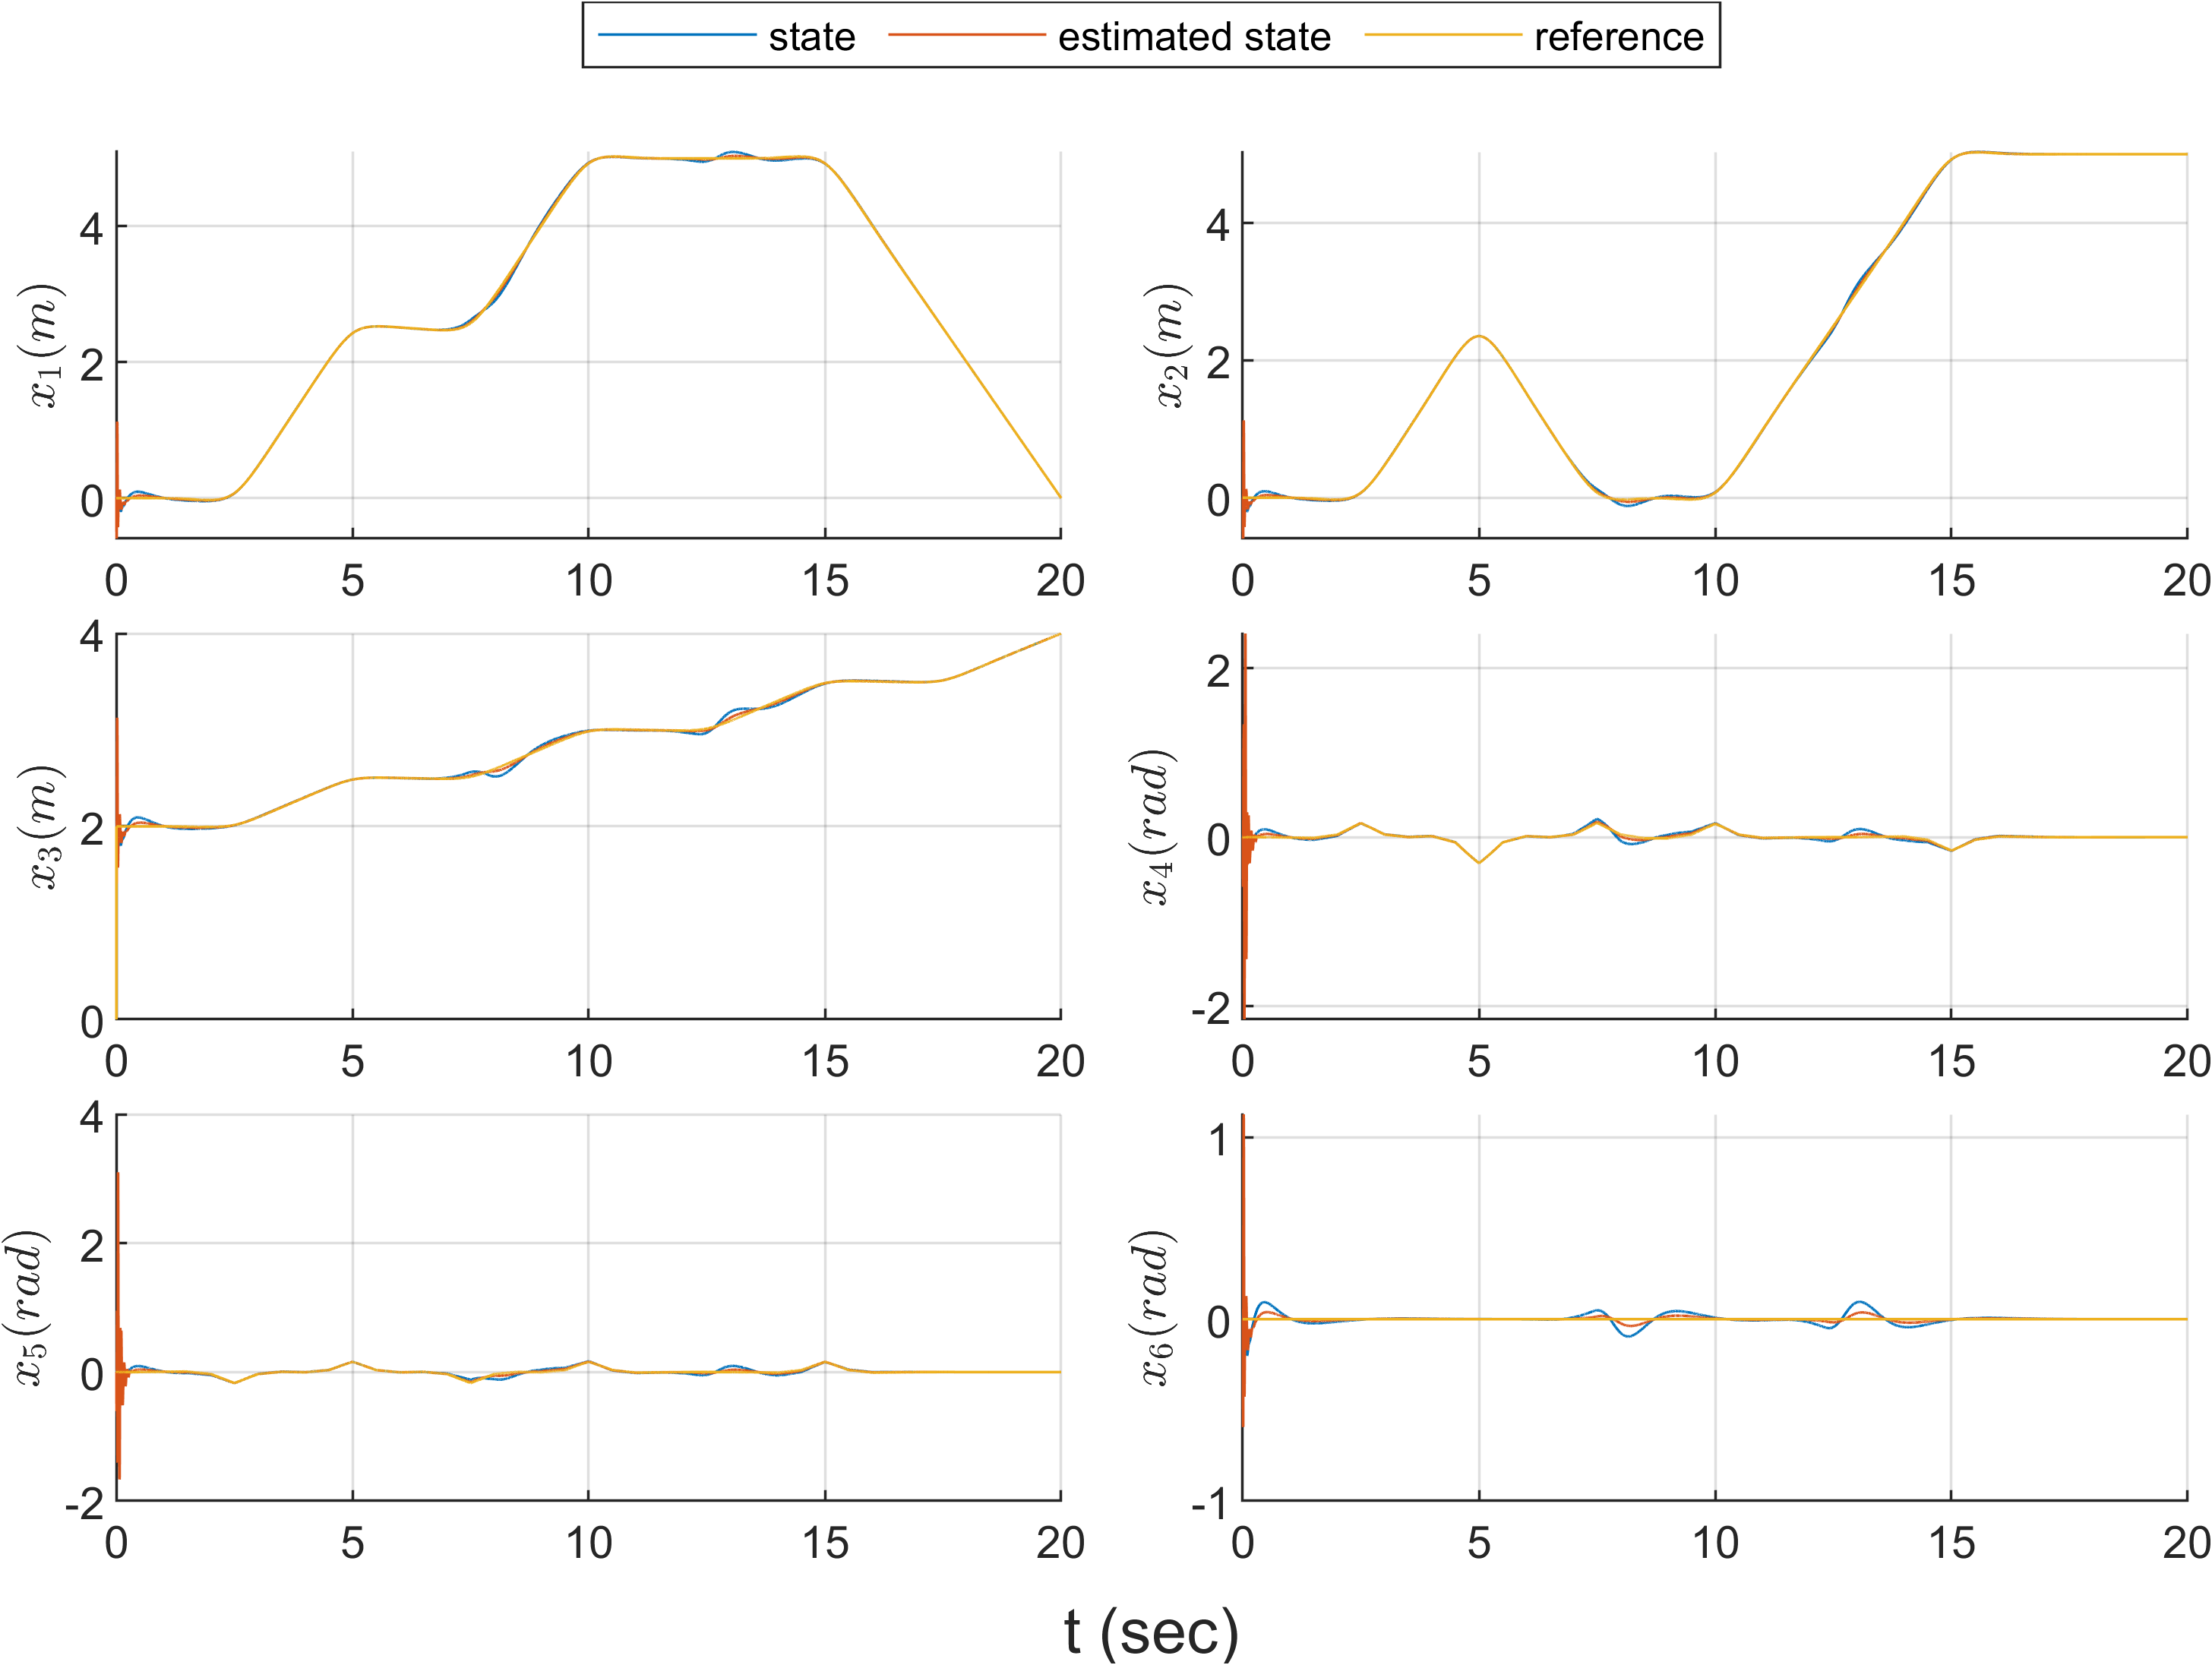
\includegraphics[scale=.57]{fig/uav (1).png}\caption{The trajectories of reference, state and estimated state of the UAV $\alpha_{1,1}$}%
    \label{fig:UAV, state}
\end{figure}
\begin{figure}[htbp]
    \centering
    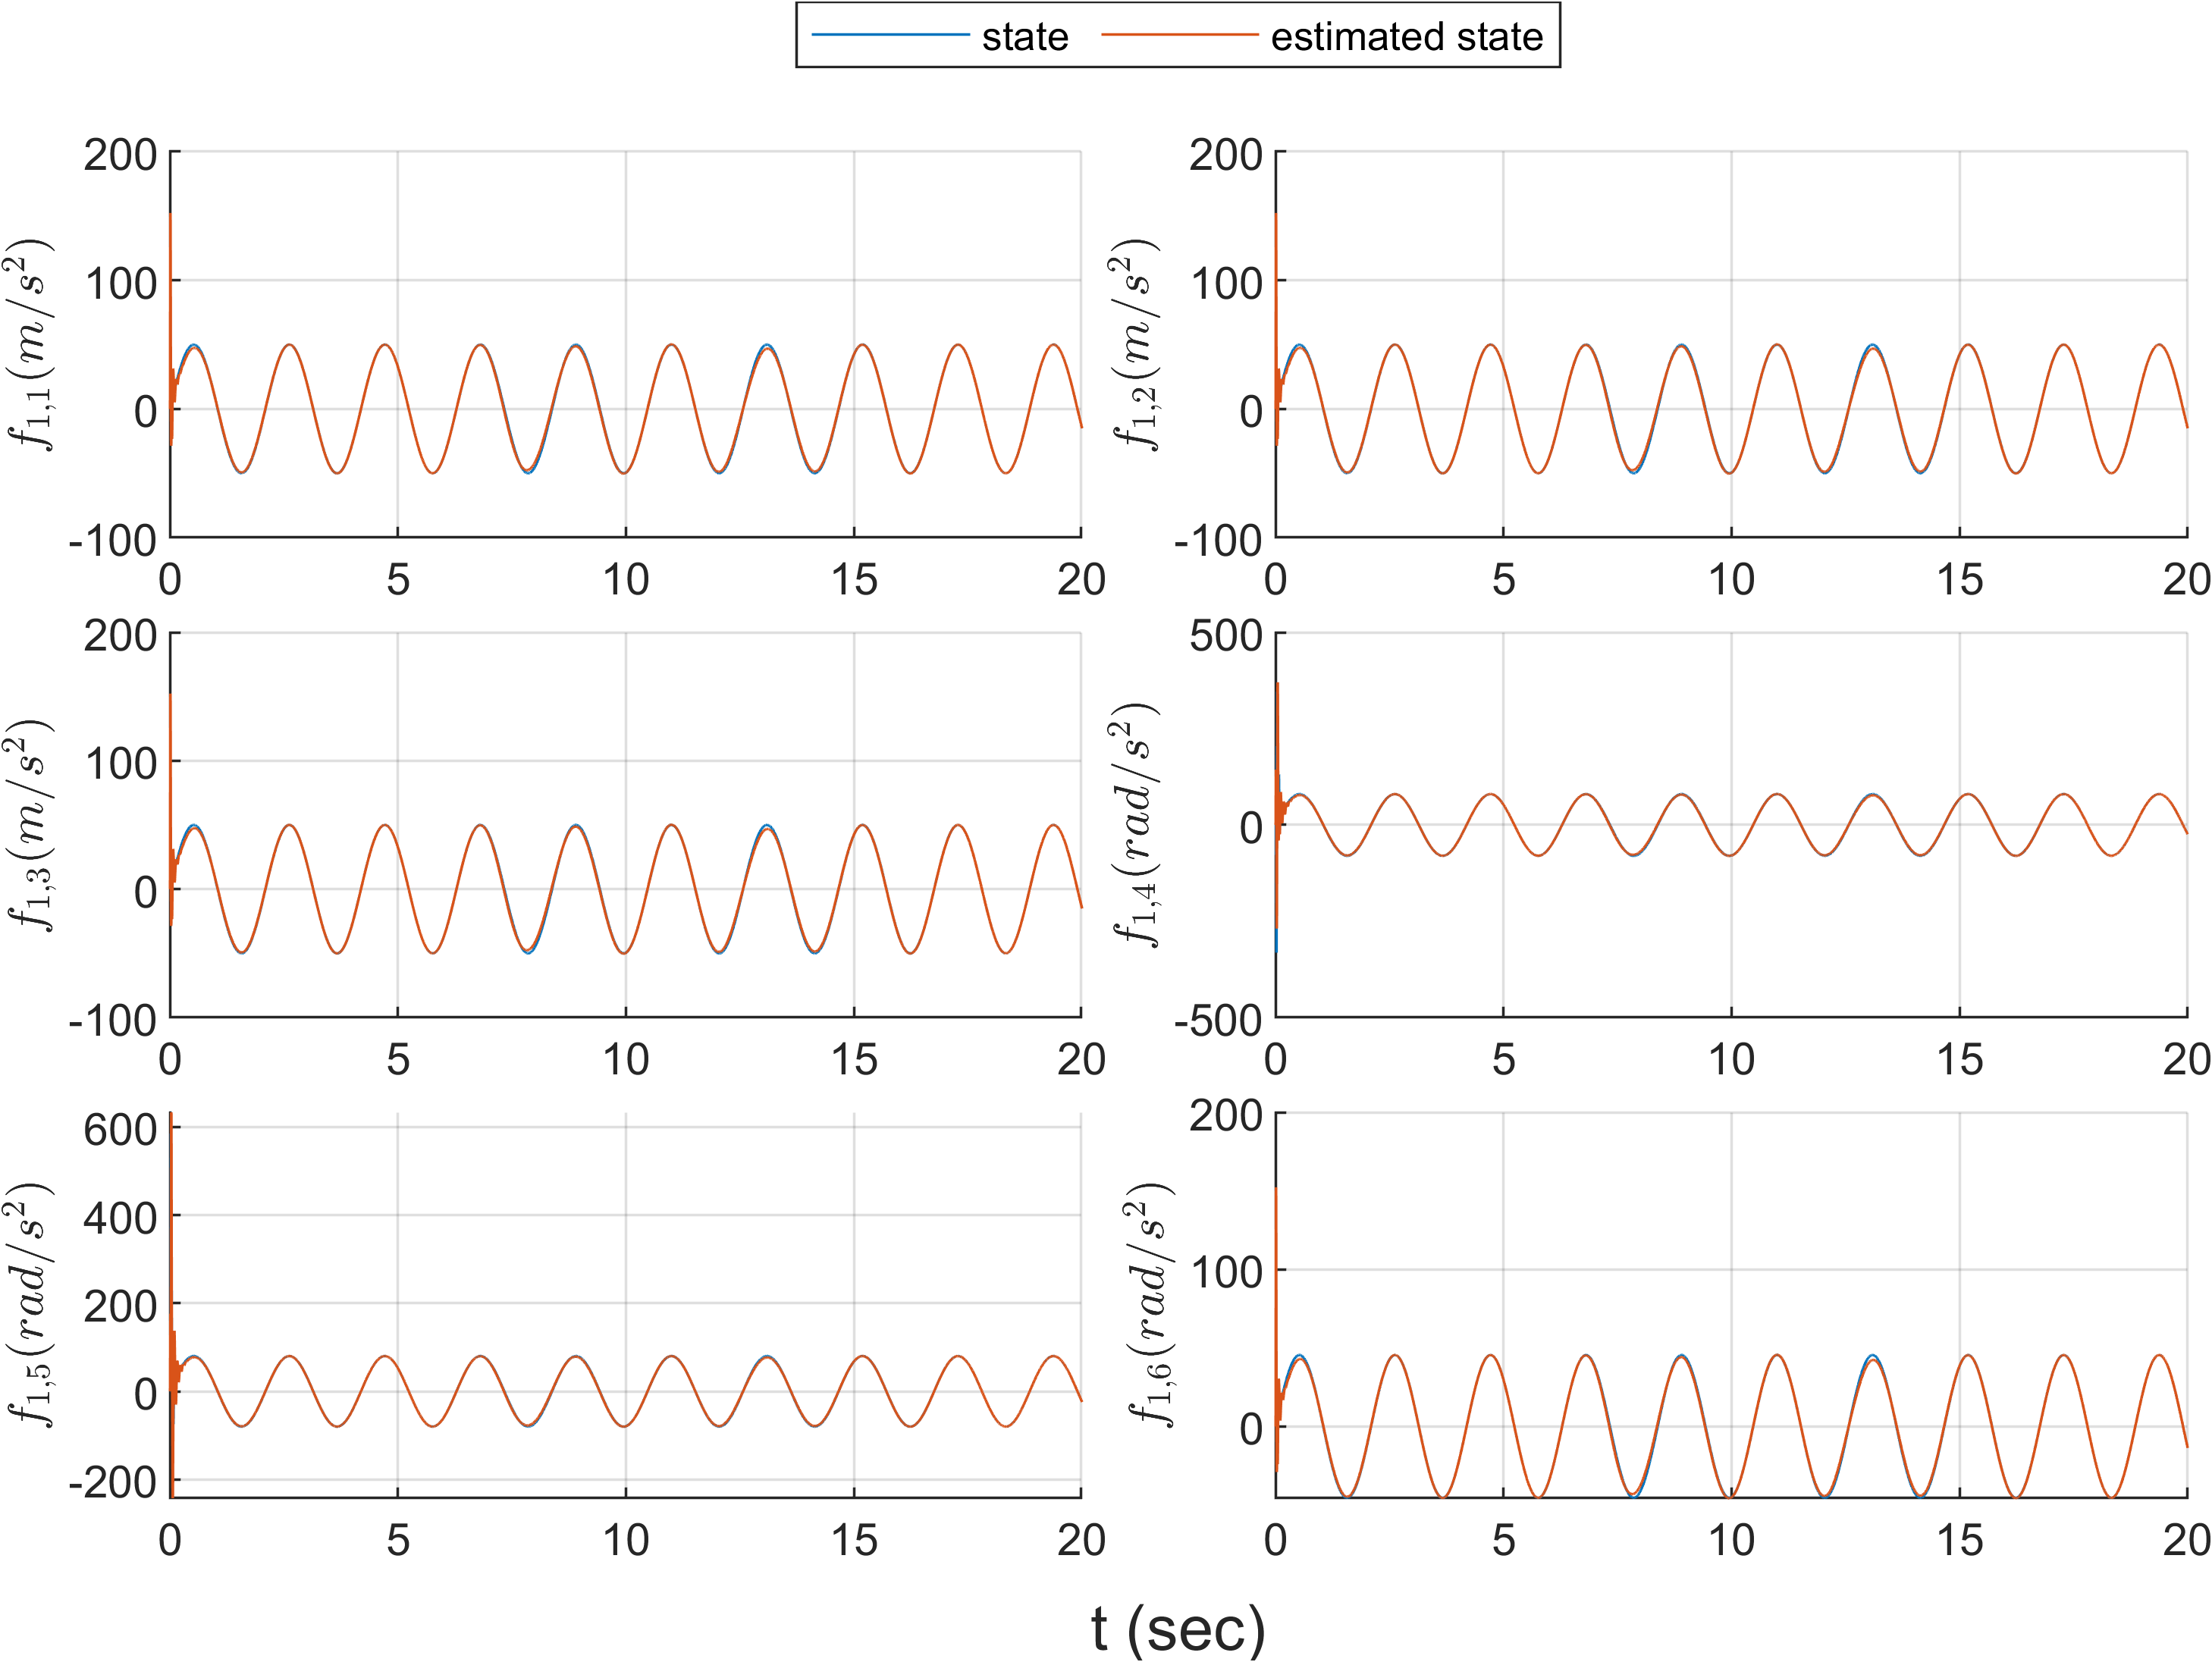
\includegraphics[scale=.57]{fig/uav (2).png}\caption{The estimation of actuator fault of the UAV $\alpha_{1,1}$}
    \label{fig:UAV, fa}
\end{figure}
\begin{figure}[htbp]
    \centering
    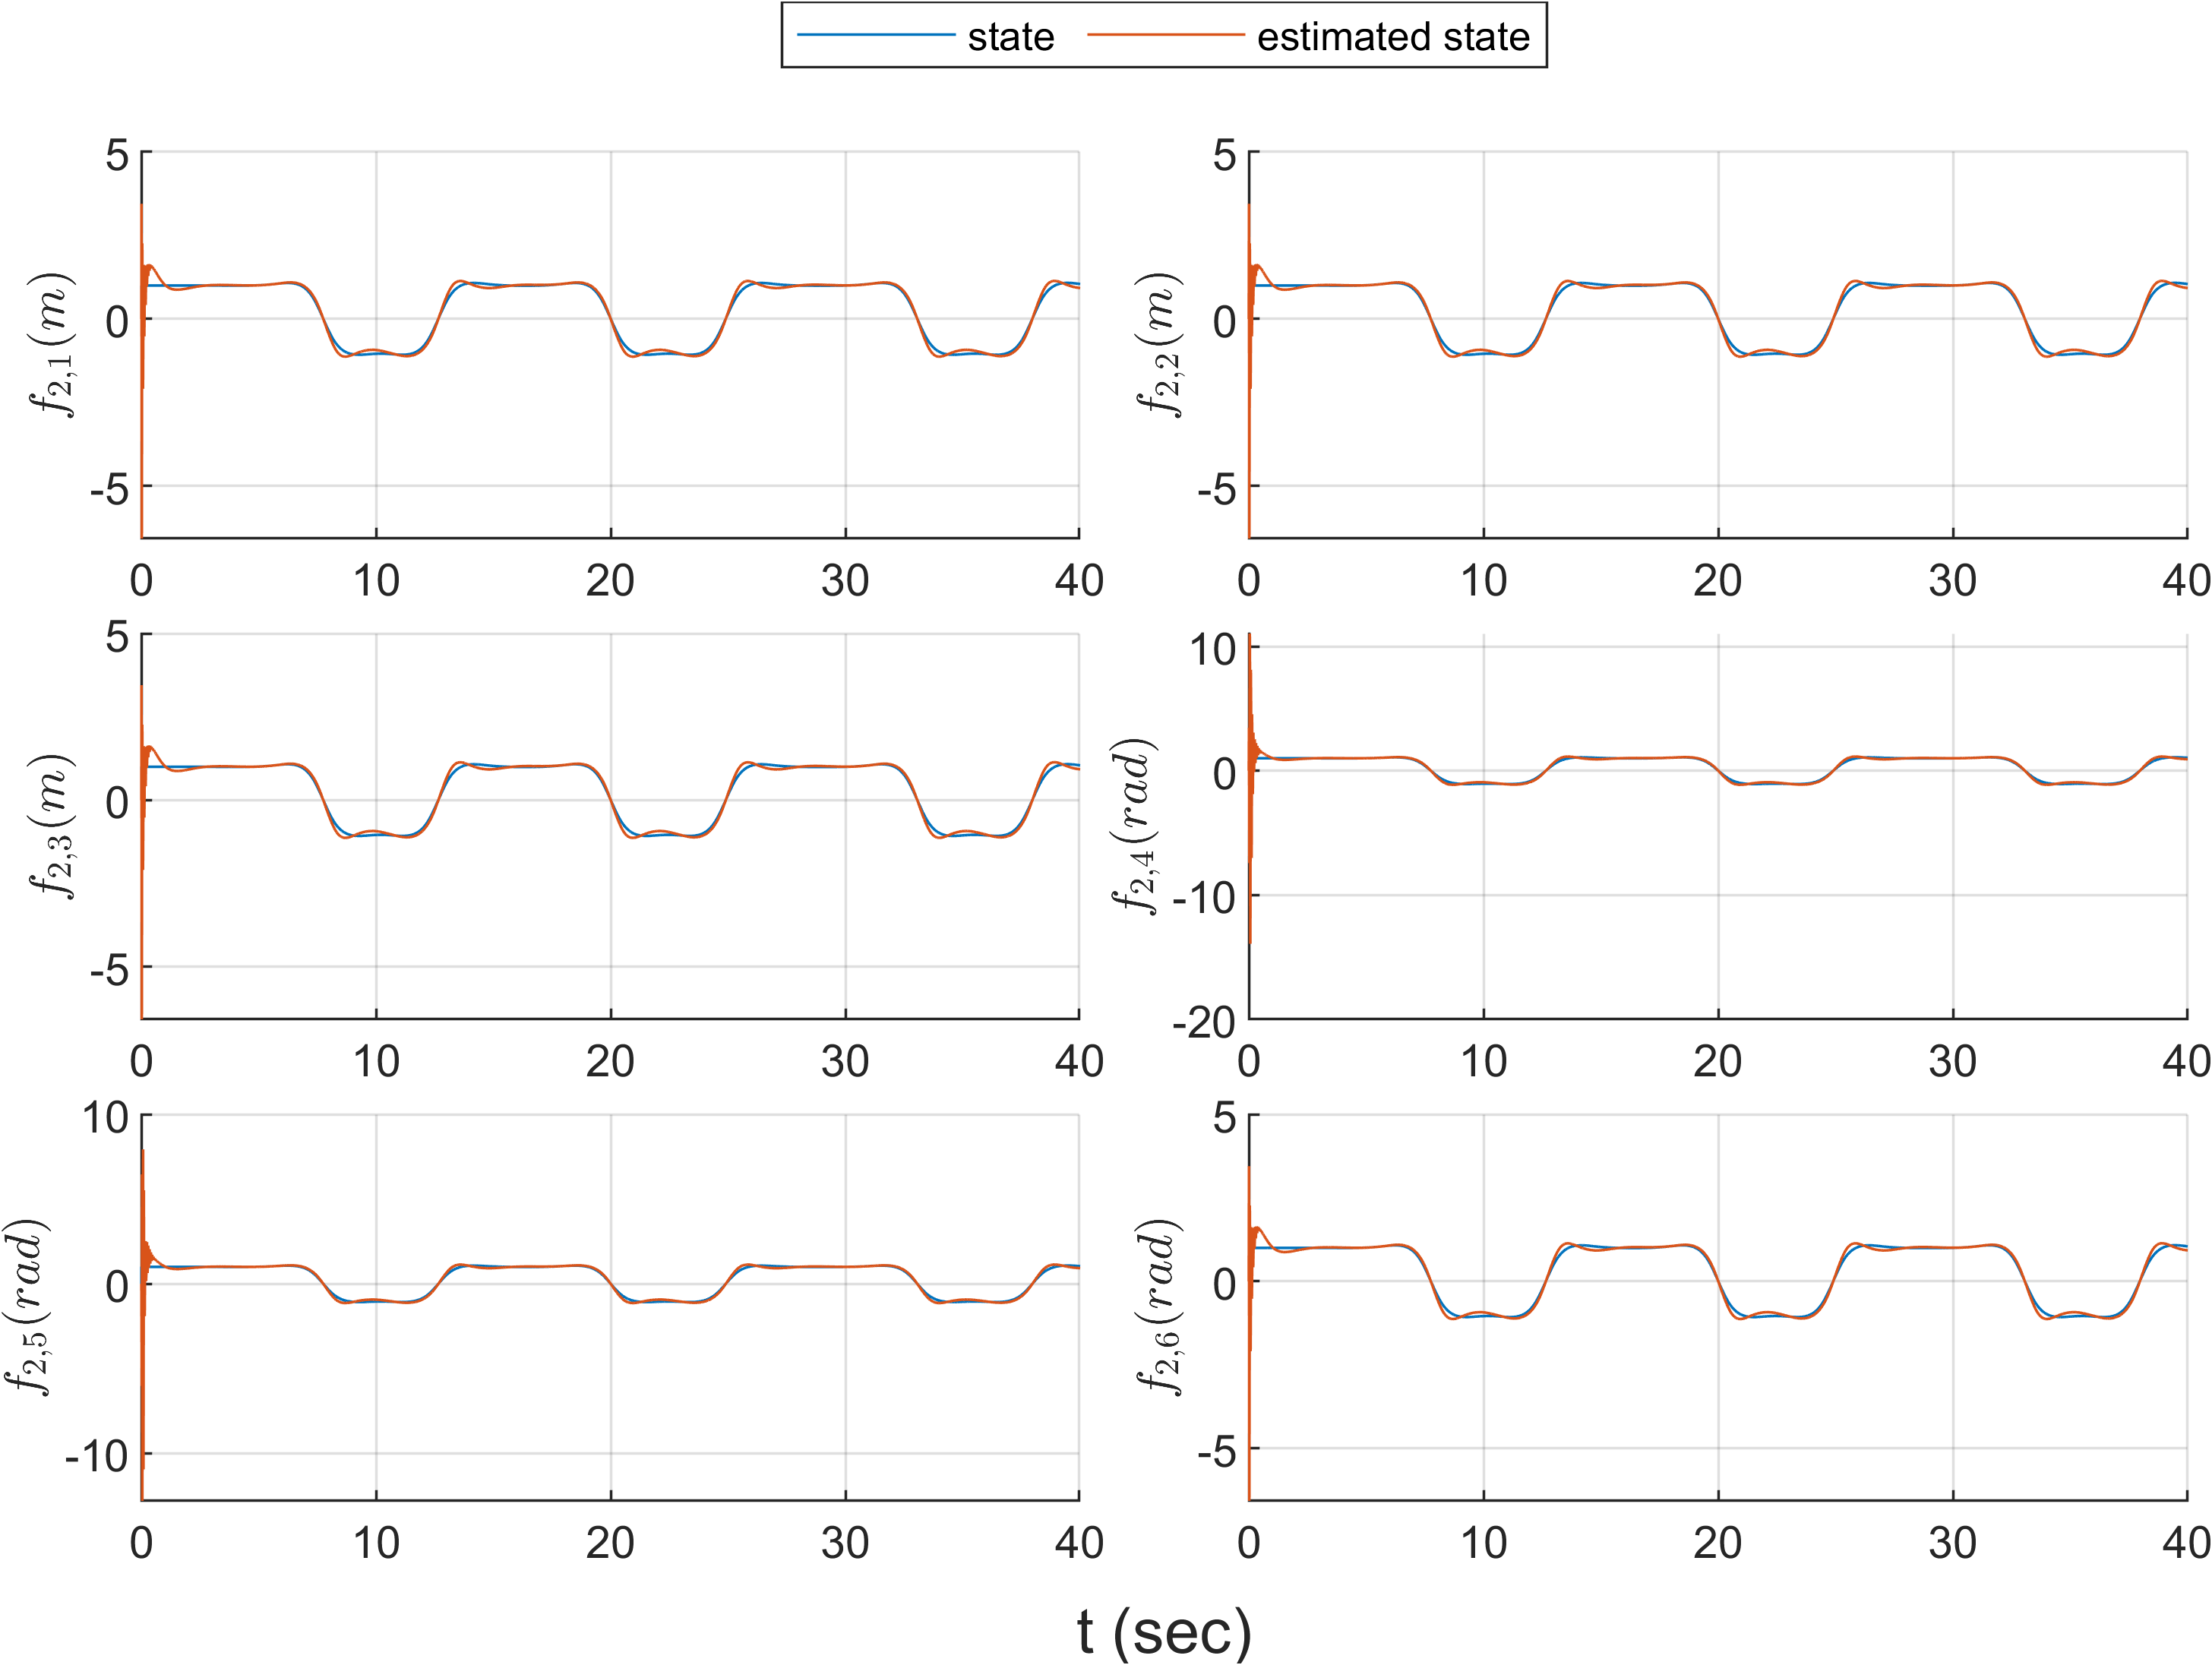
\includegraphics[scale=.57]{fig/uav (3).png}\caption{The estimation of sensor fault of the UAV $\alpha_{1,1}$}%
    \label{fig:UAV, fs}
\end{figure}
\begin{figure}[htbp]
    \centering
    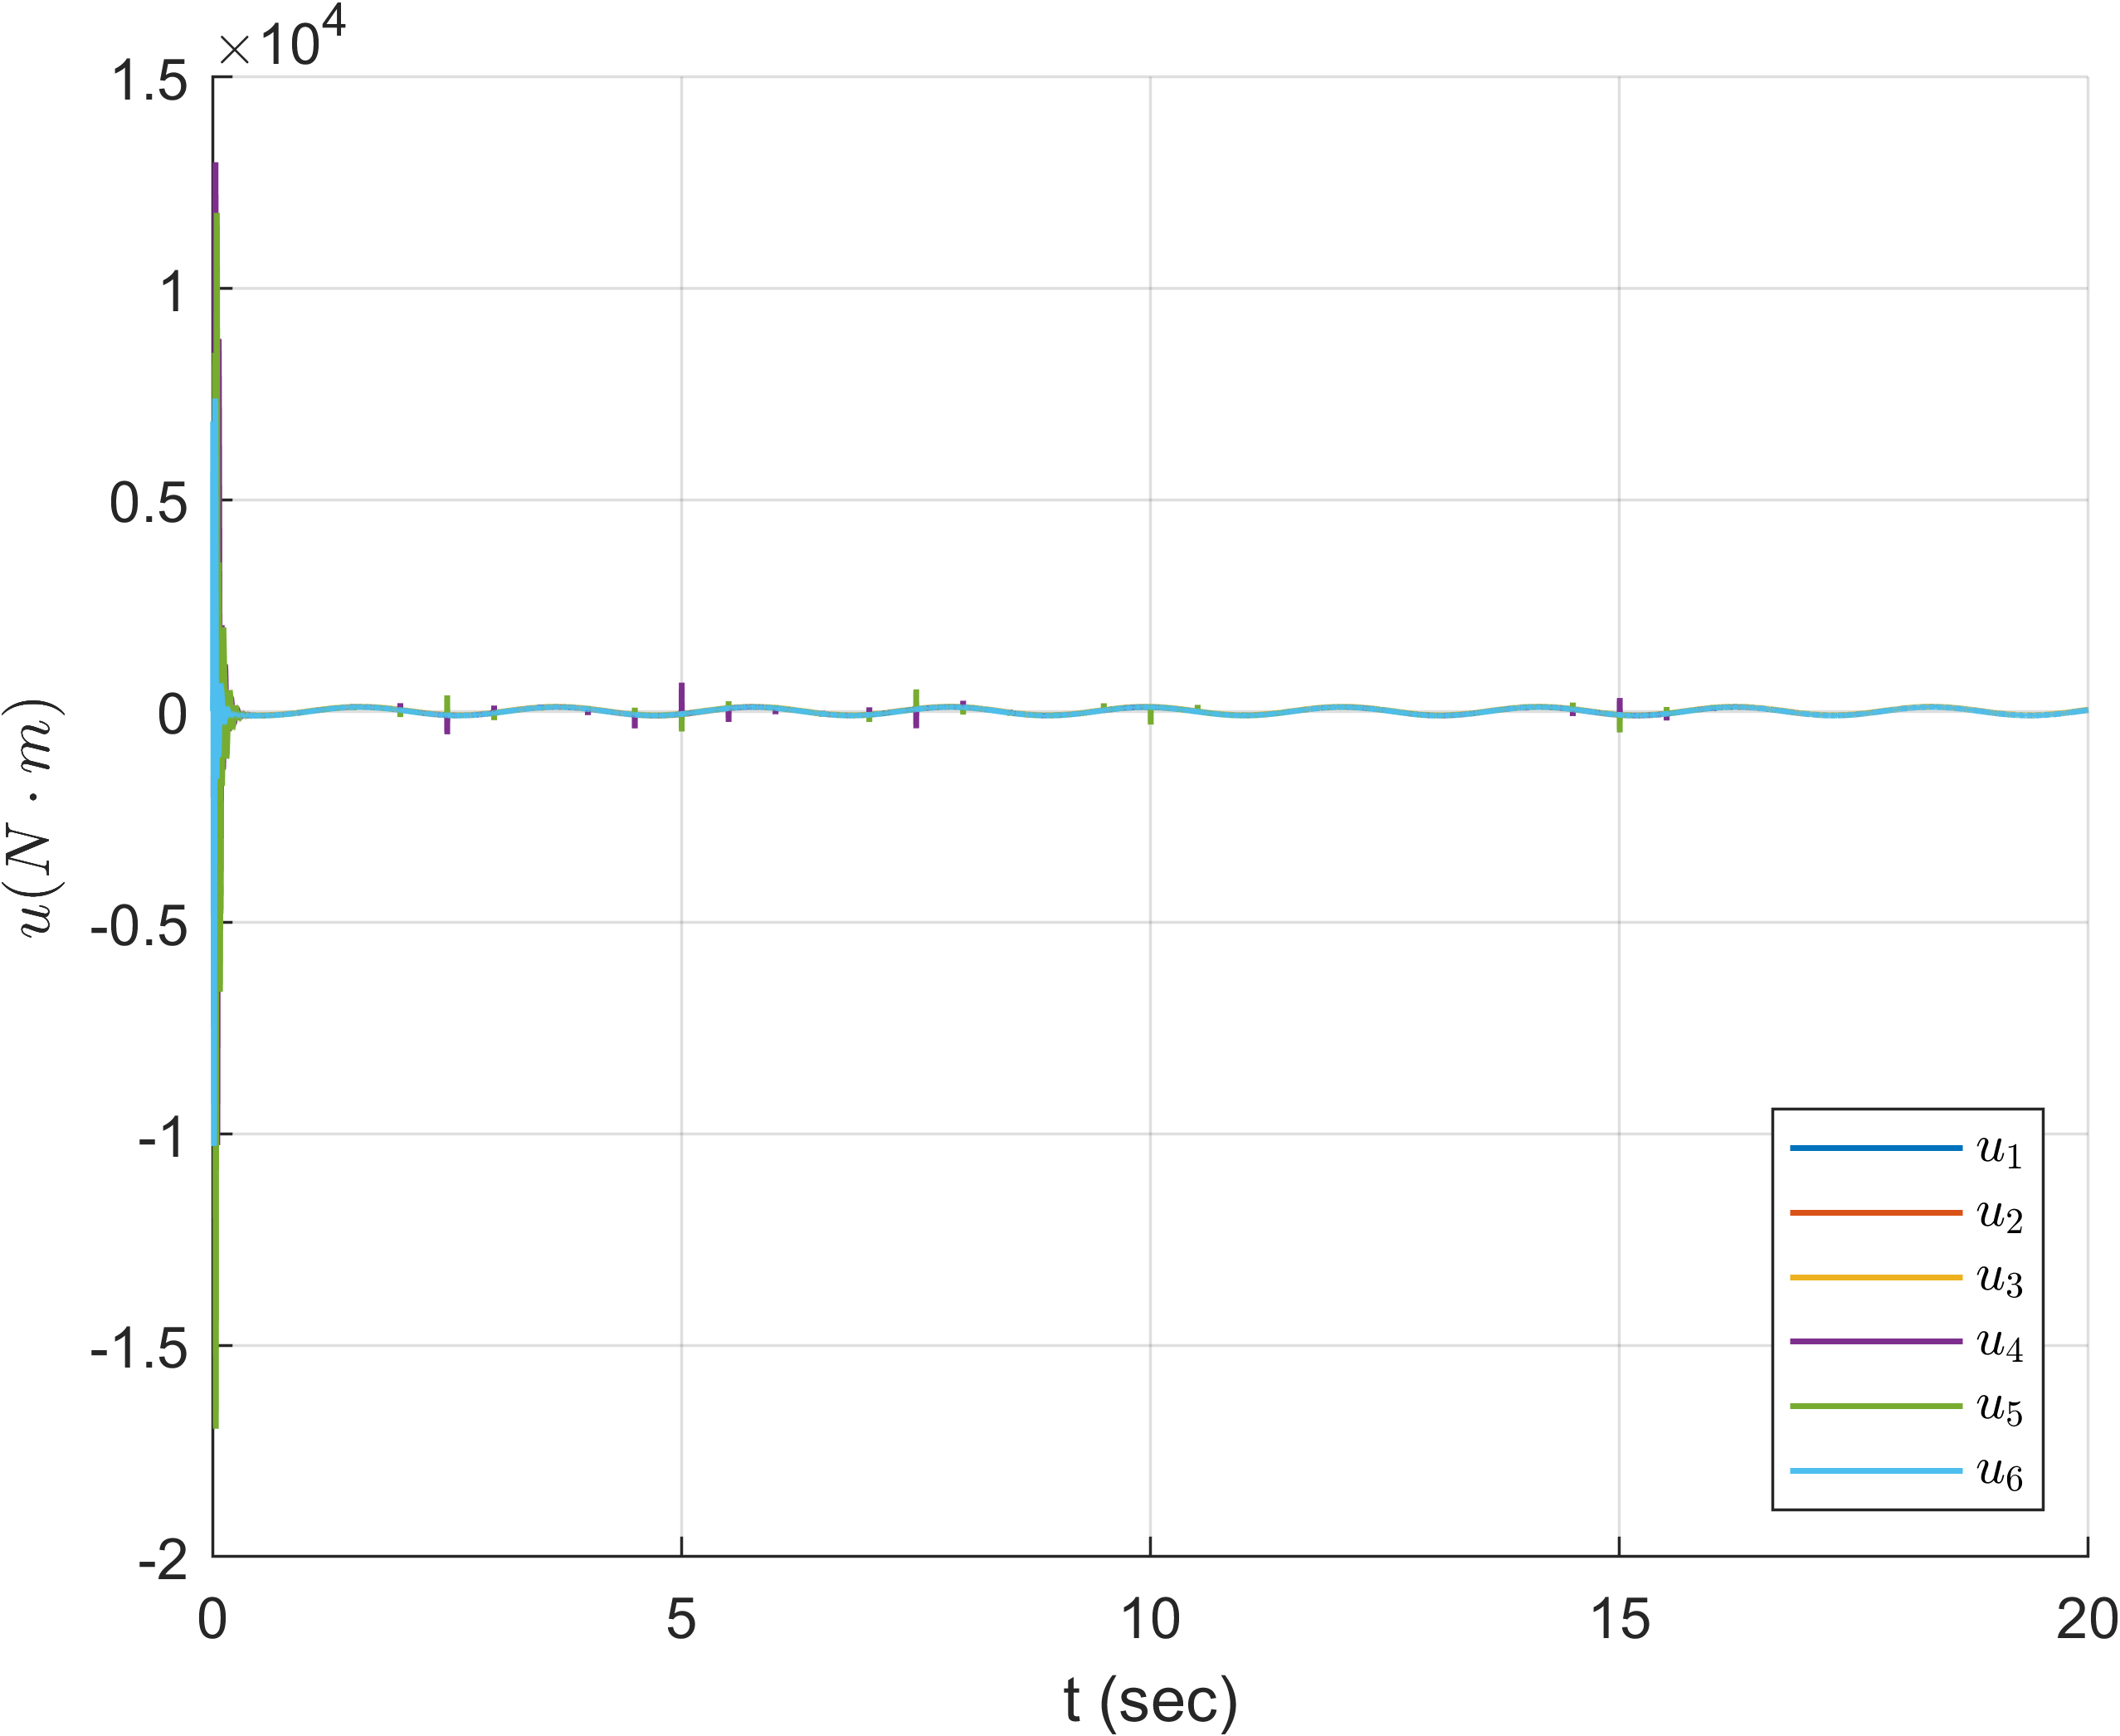
\includegraphics[scale=.57]{fig/uav (4).png}\caption{The control effort of the UAV $\alpha_{1,1}$}%
    \label{fig:UAV, control}
\end{figure}

\textit{Robot $\alpha_{1,2}$:}
The trajectories of reference, state and estimated state are shown in Fig. \ref{fig:robot, state}. The estimation of actuator fault $f_1(t)$ is shown in Fig. \ref{fig:robot, fa}. The estimation of sensor fault $f_2(t)$ is shown in Fig. \ref{fig:robot, fs}. The control effort is shown in Fig. \ref{fig:robot, control}.
\begin{figure}[htbp]
    \centering
    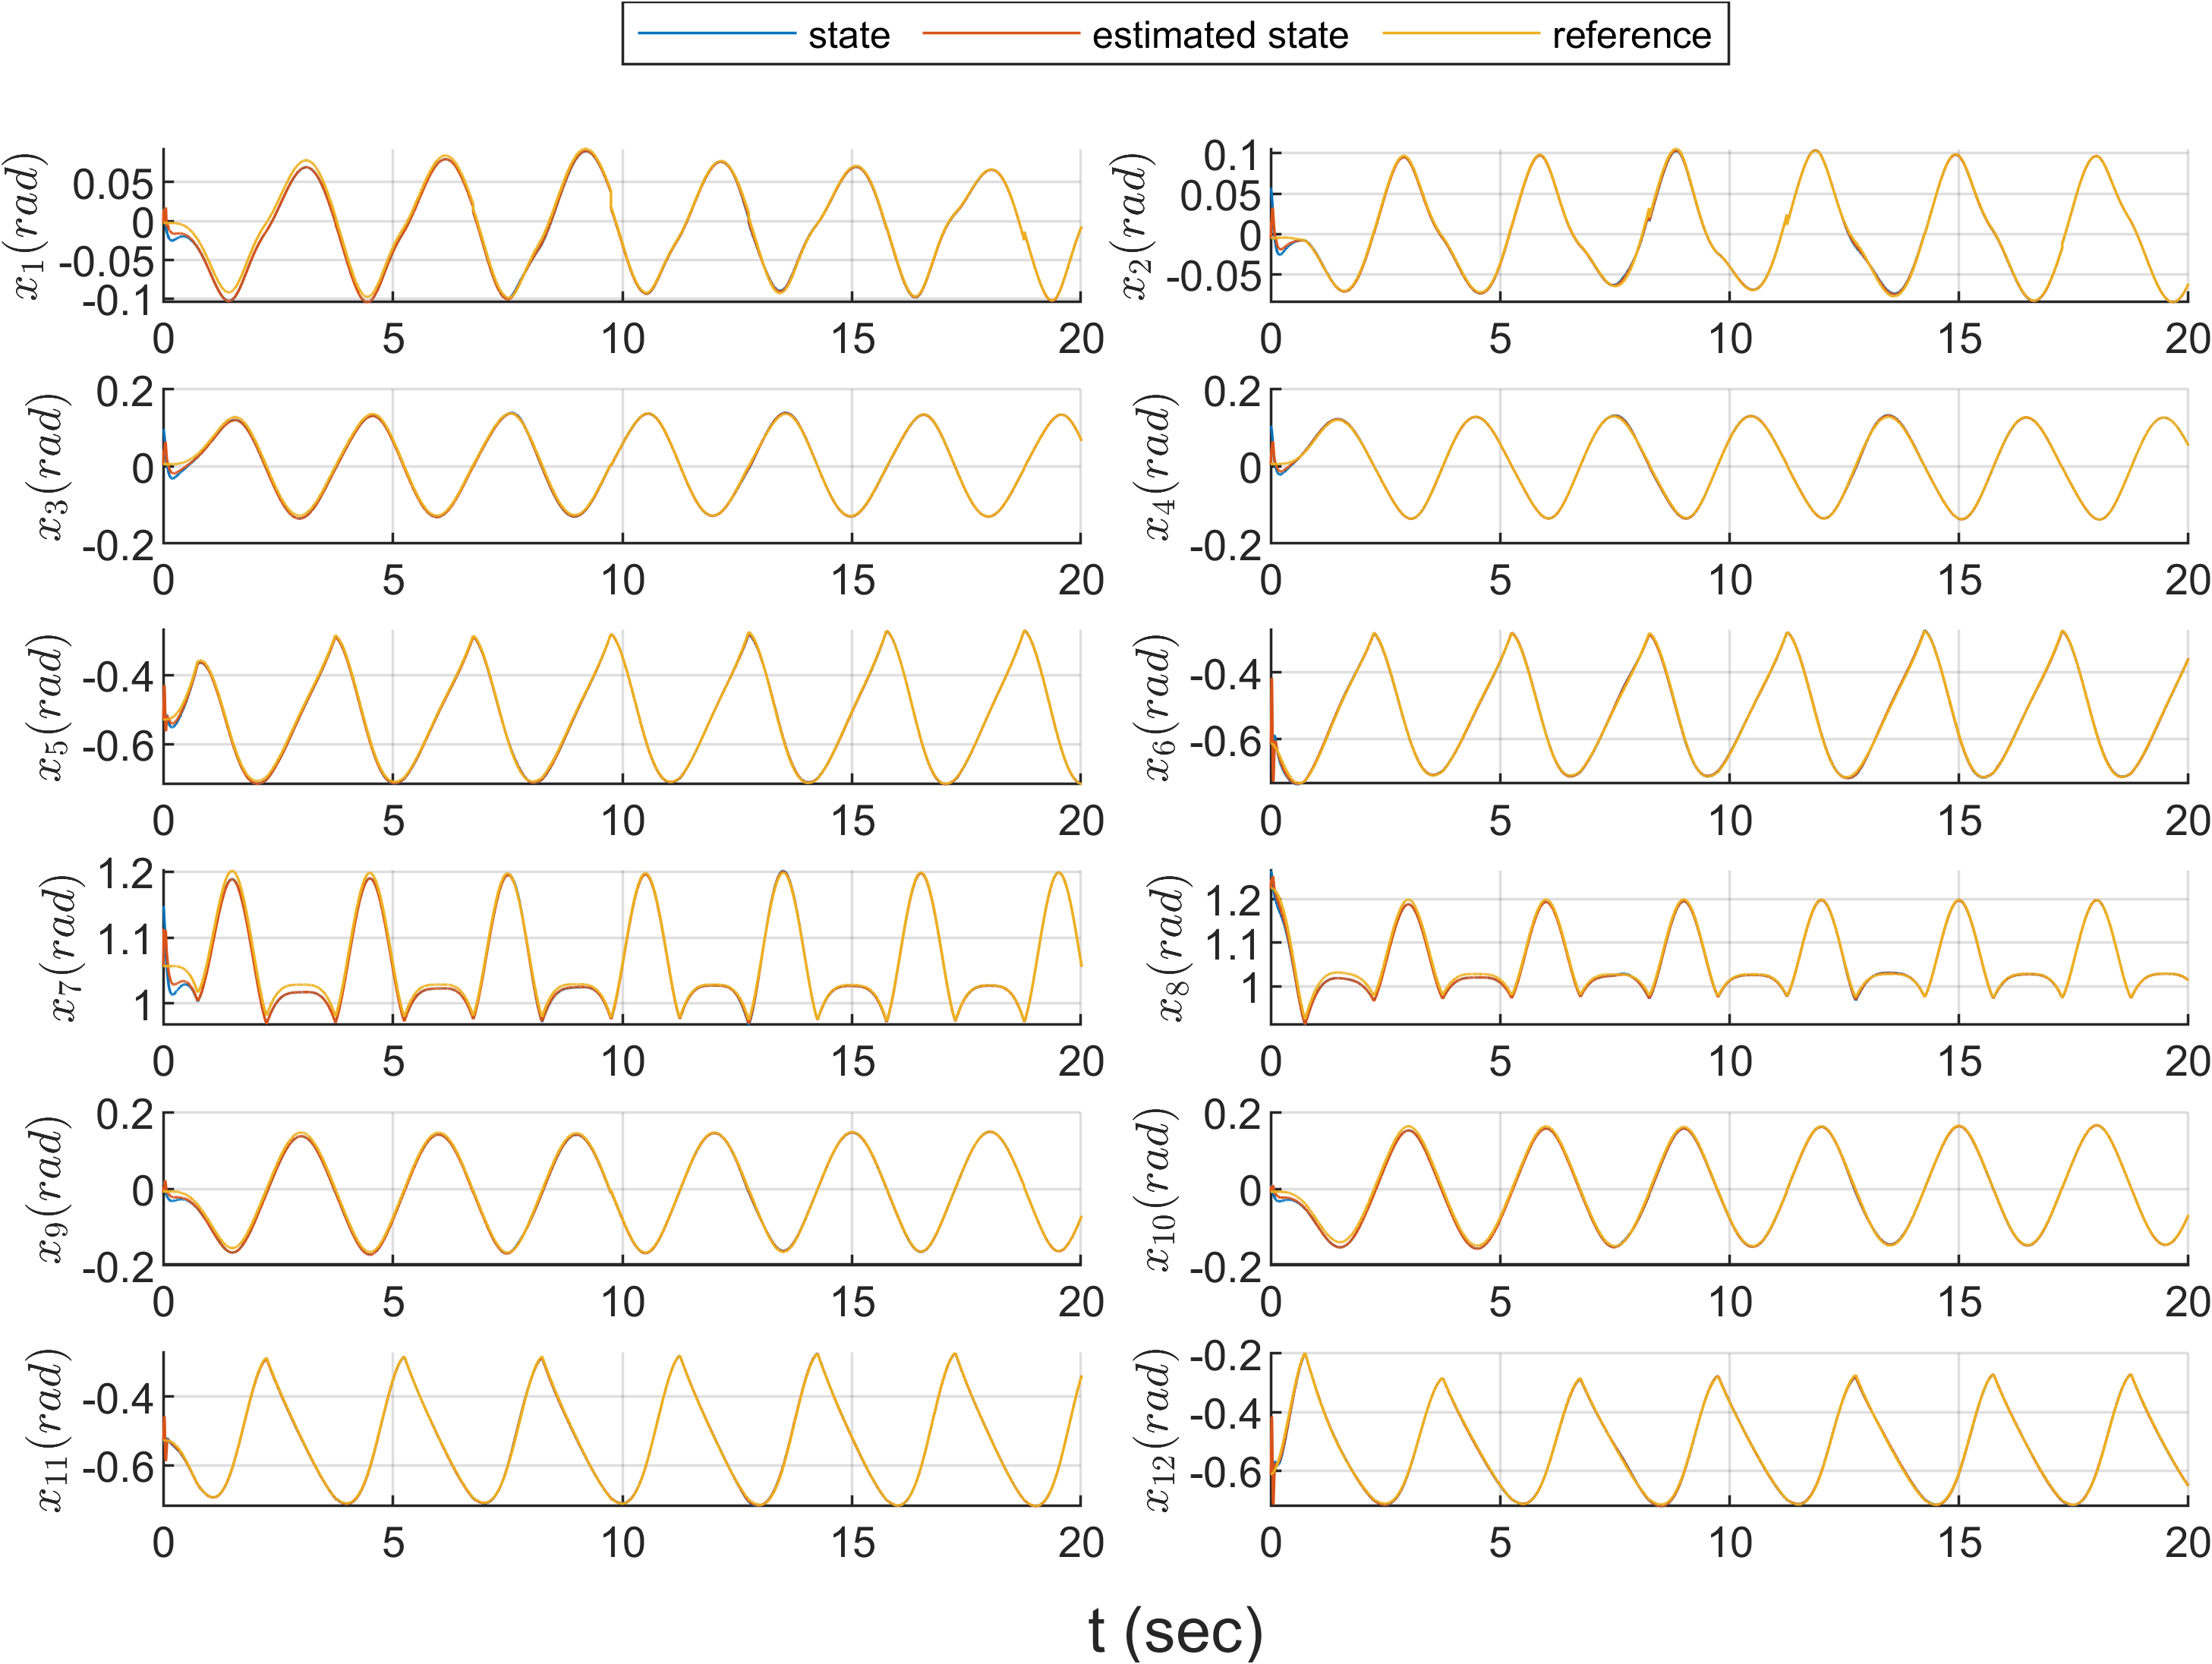
\includegraphics[scale=.57]{fig/robot (1).png}\caption{The trajectories of reference, state and estimated state of the robot $\alpha_{1,2}$}%
    \label{fig:robot, state}
\end{figure}
\begin{figure}[htbp]
    \centering
    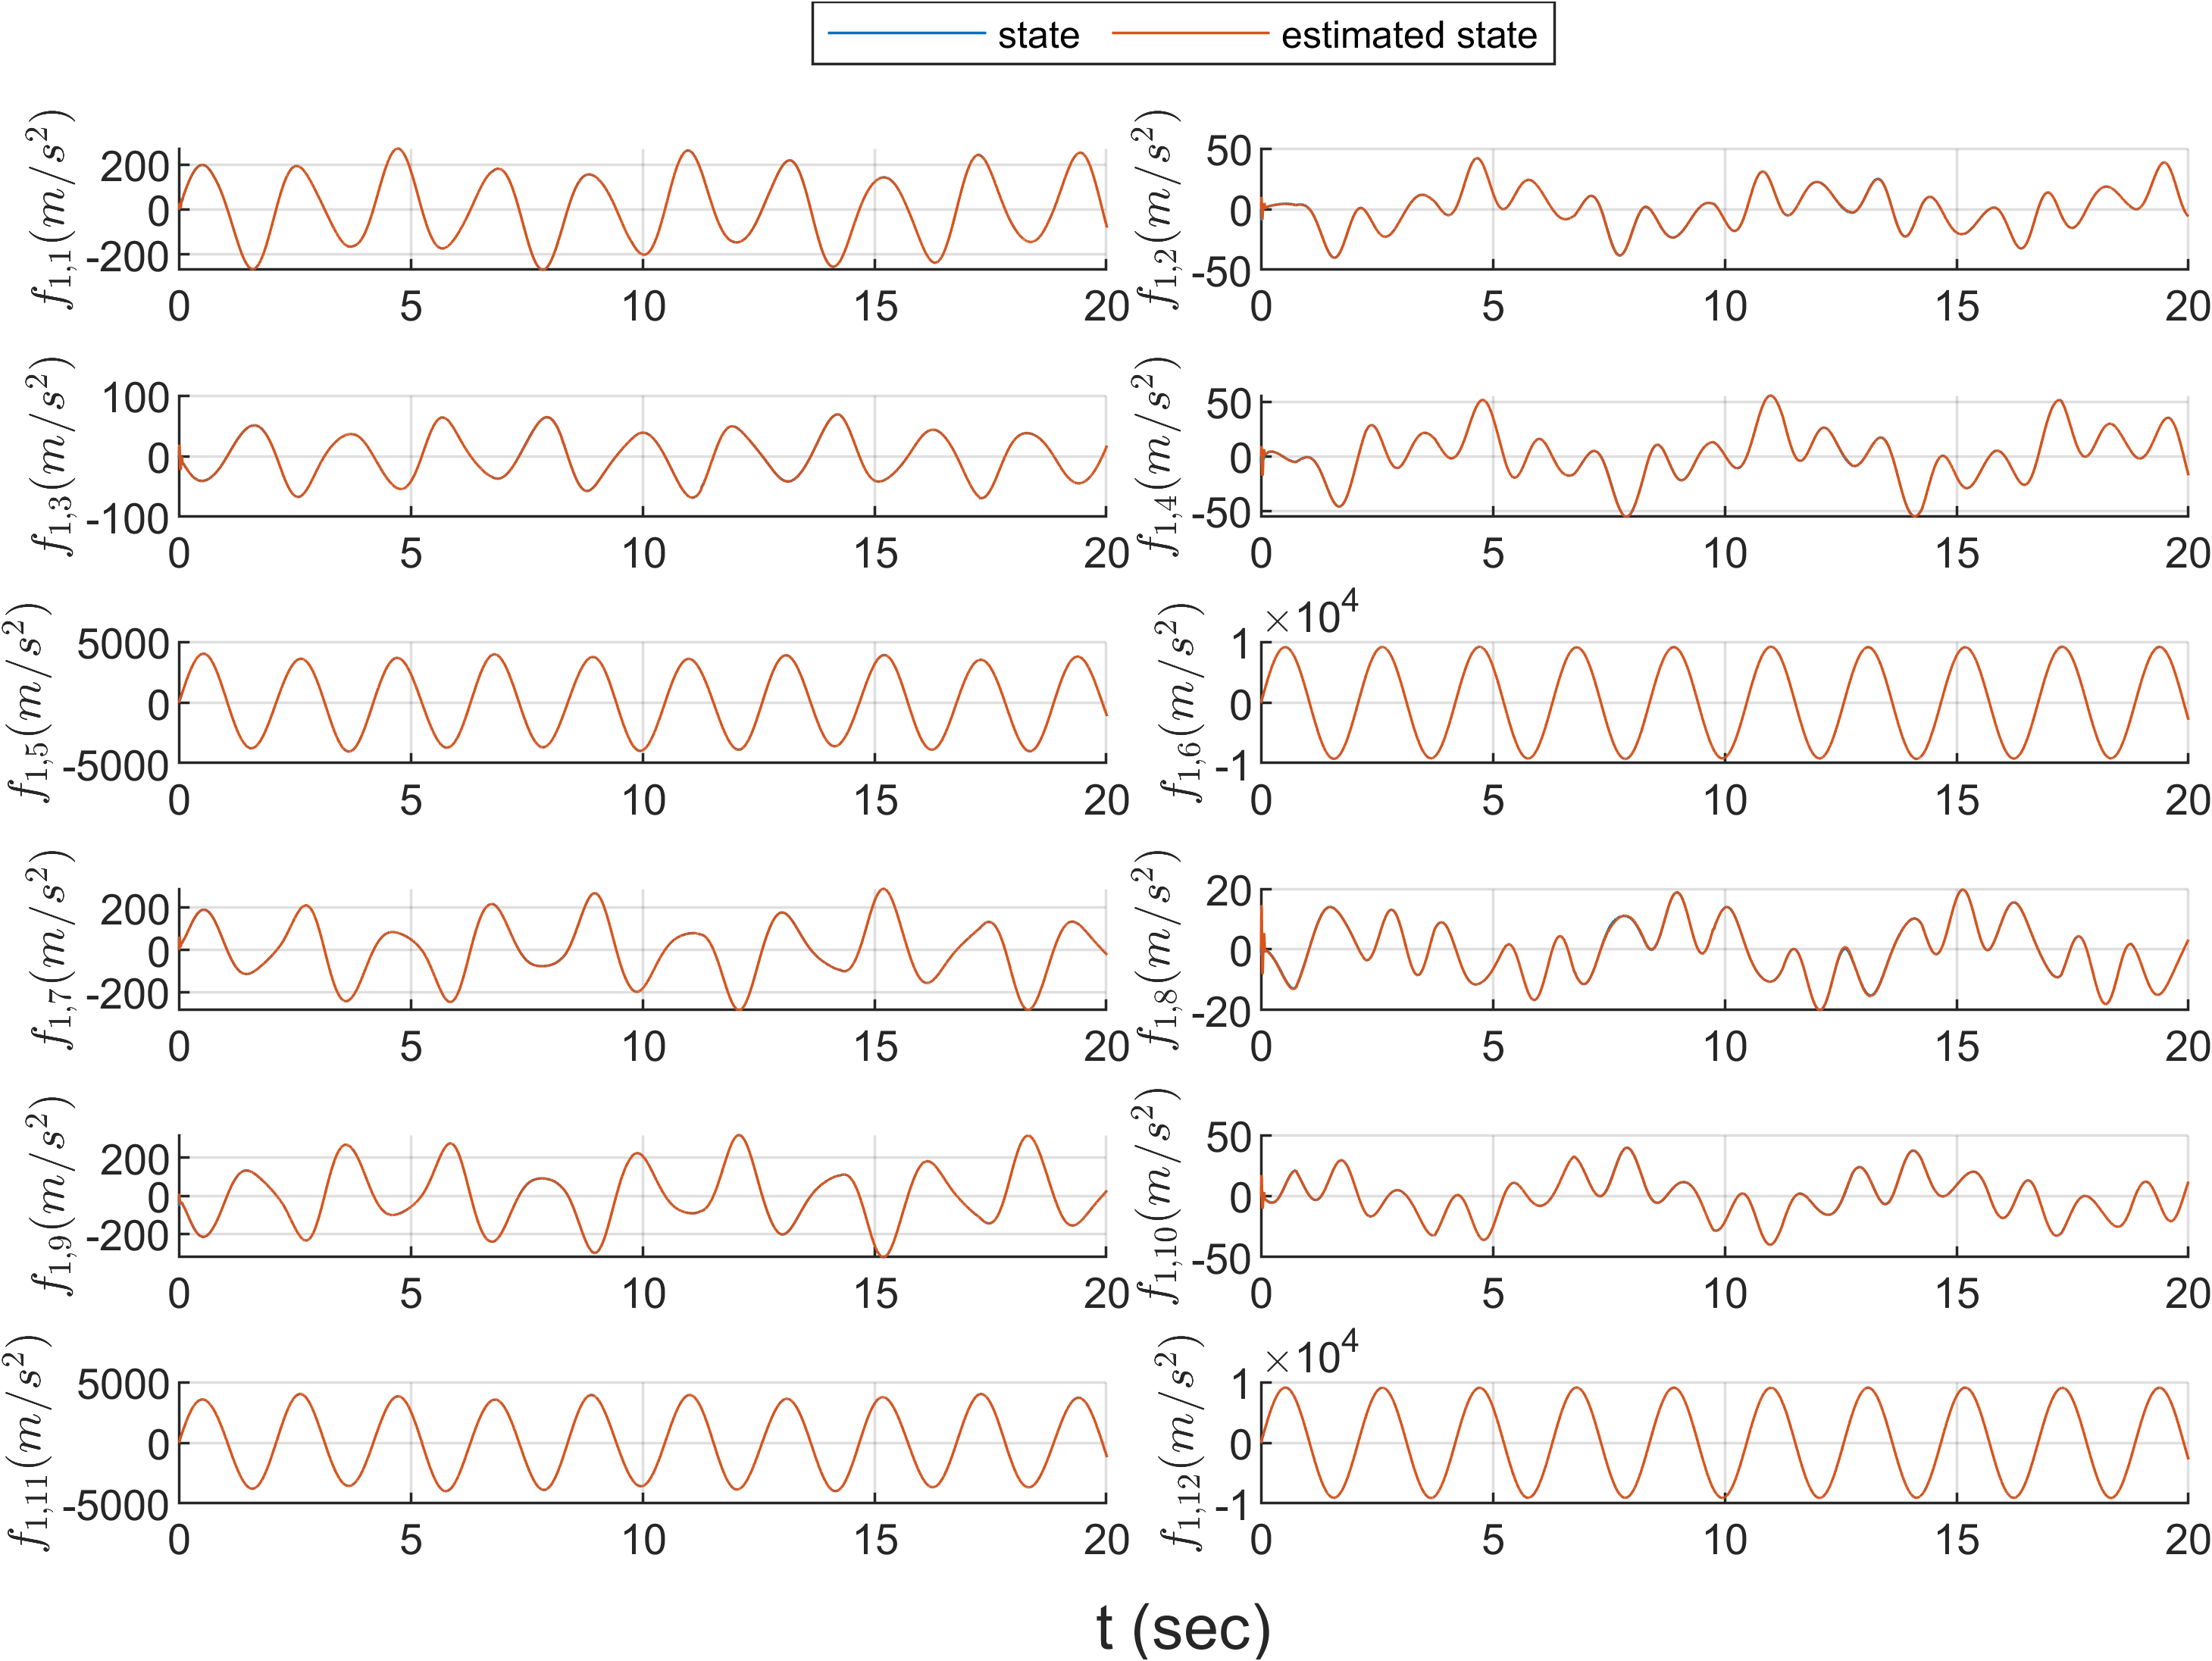
\includegraphics[scale=.57]{fig/robot (2).png}\caption{The estimation of actuator fault of the robot $\alpha_{1,2}$.}%
    \label{fig:robot, fa}
\end{figure}
\begin{figure}[htbp]
    \centering
    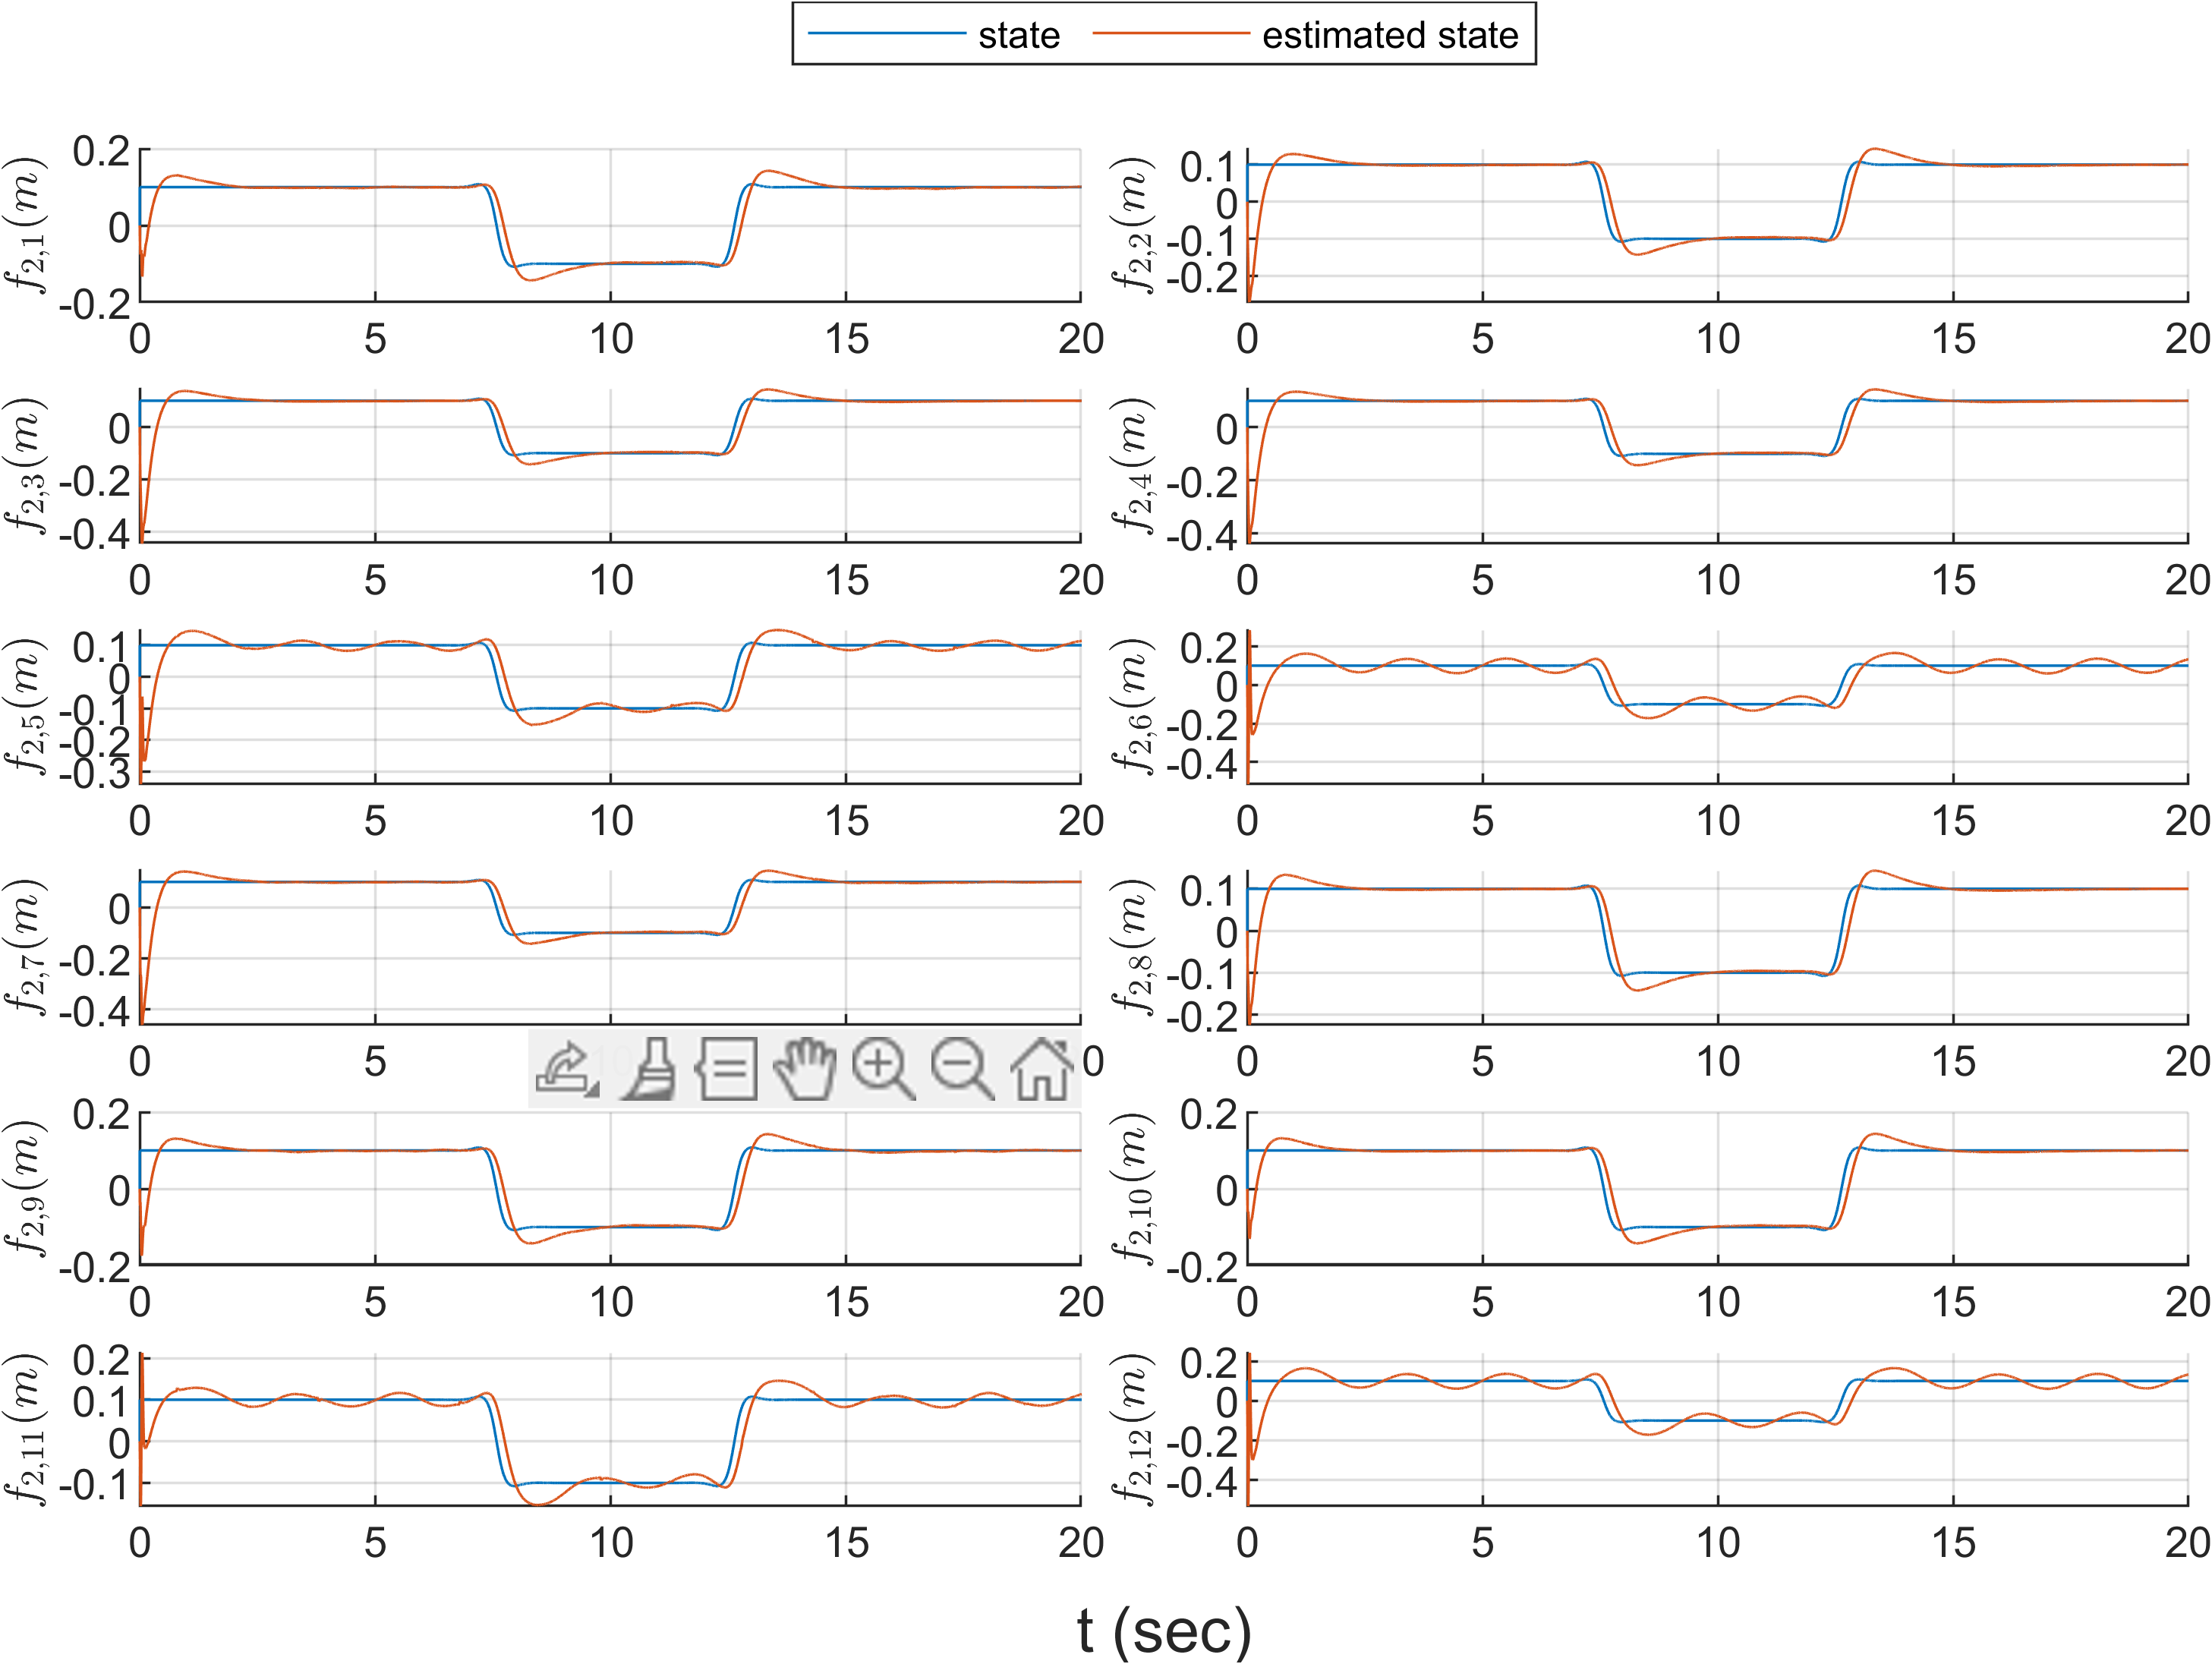
\includegraphics[scale=.57]{fig/robot (3).png}\caption{The estimation of sensor fault of the robot $\alpha_{1,2}$}%
    \label{fig:robot, fs}
\end{figure}
\begin{figure}[htbp]
    \centering
    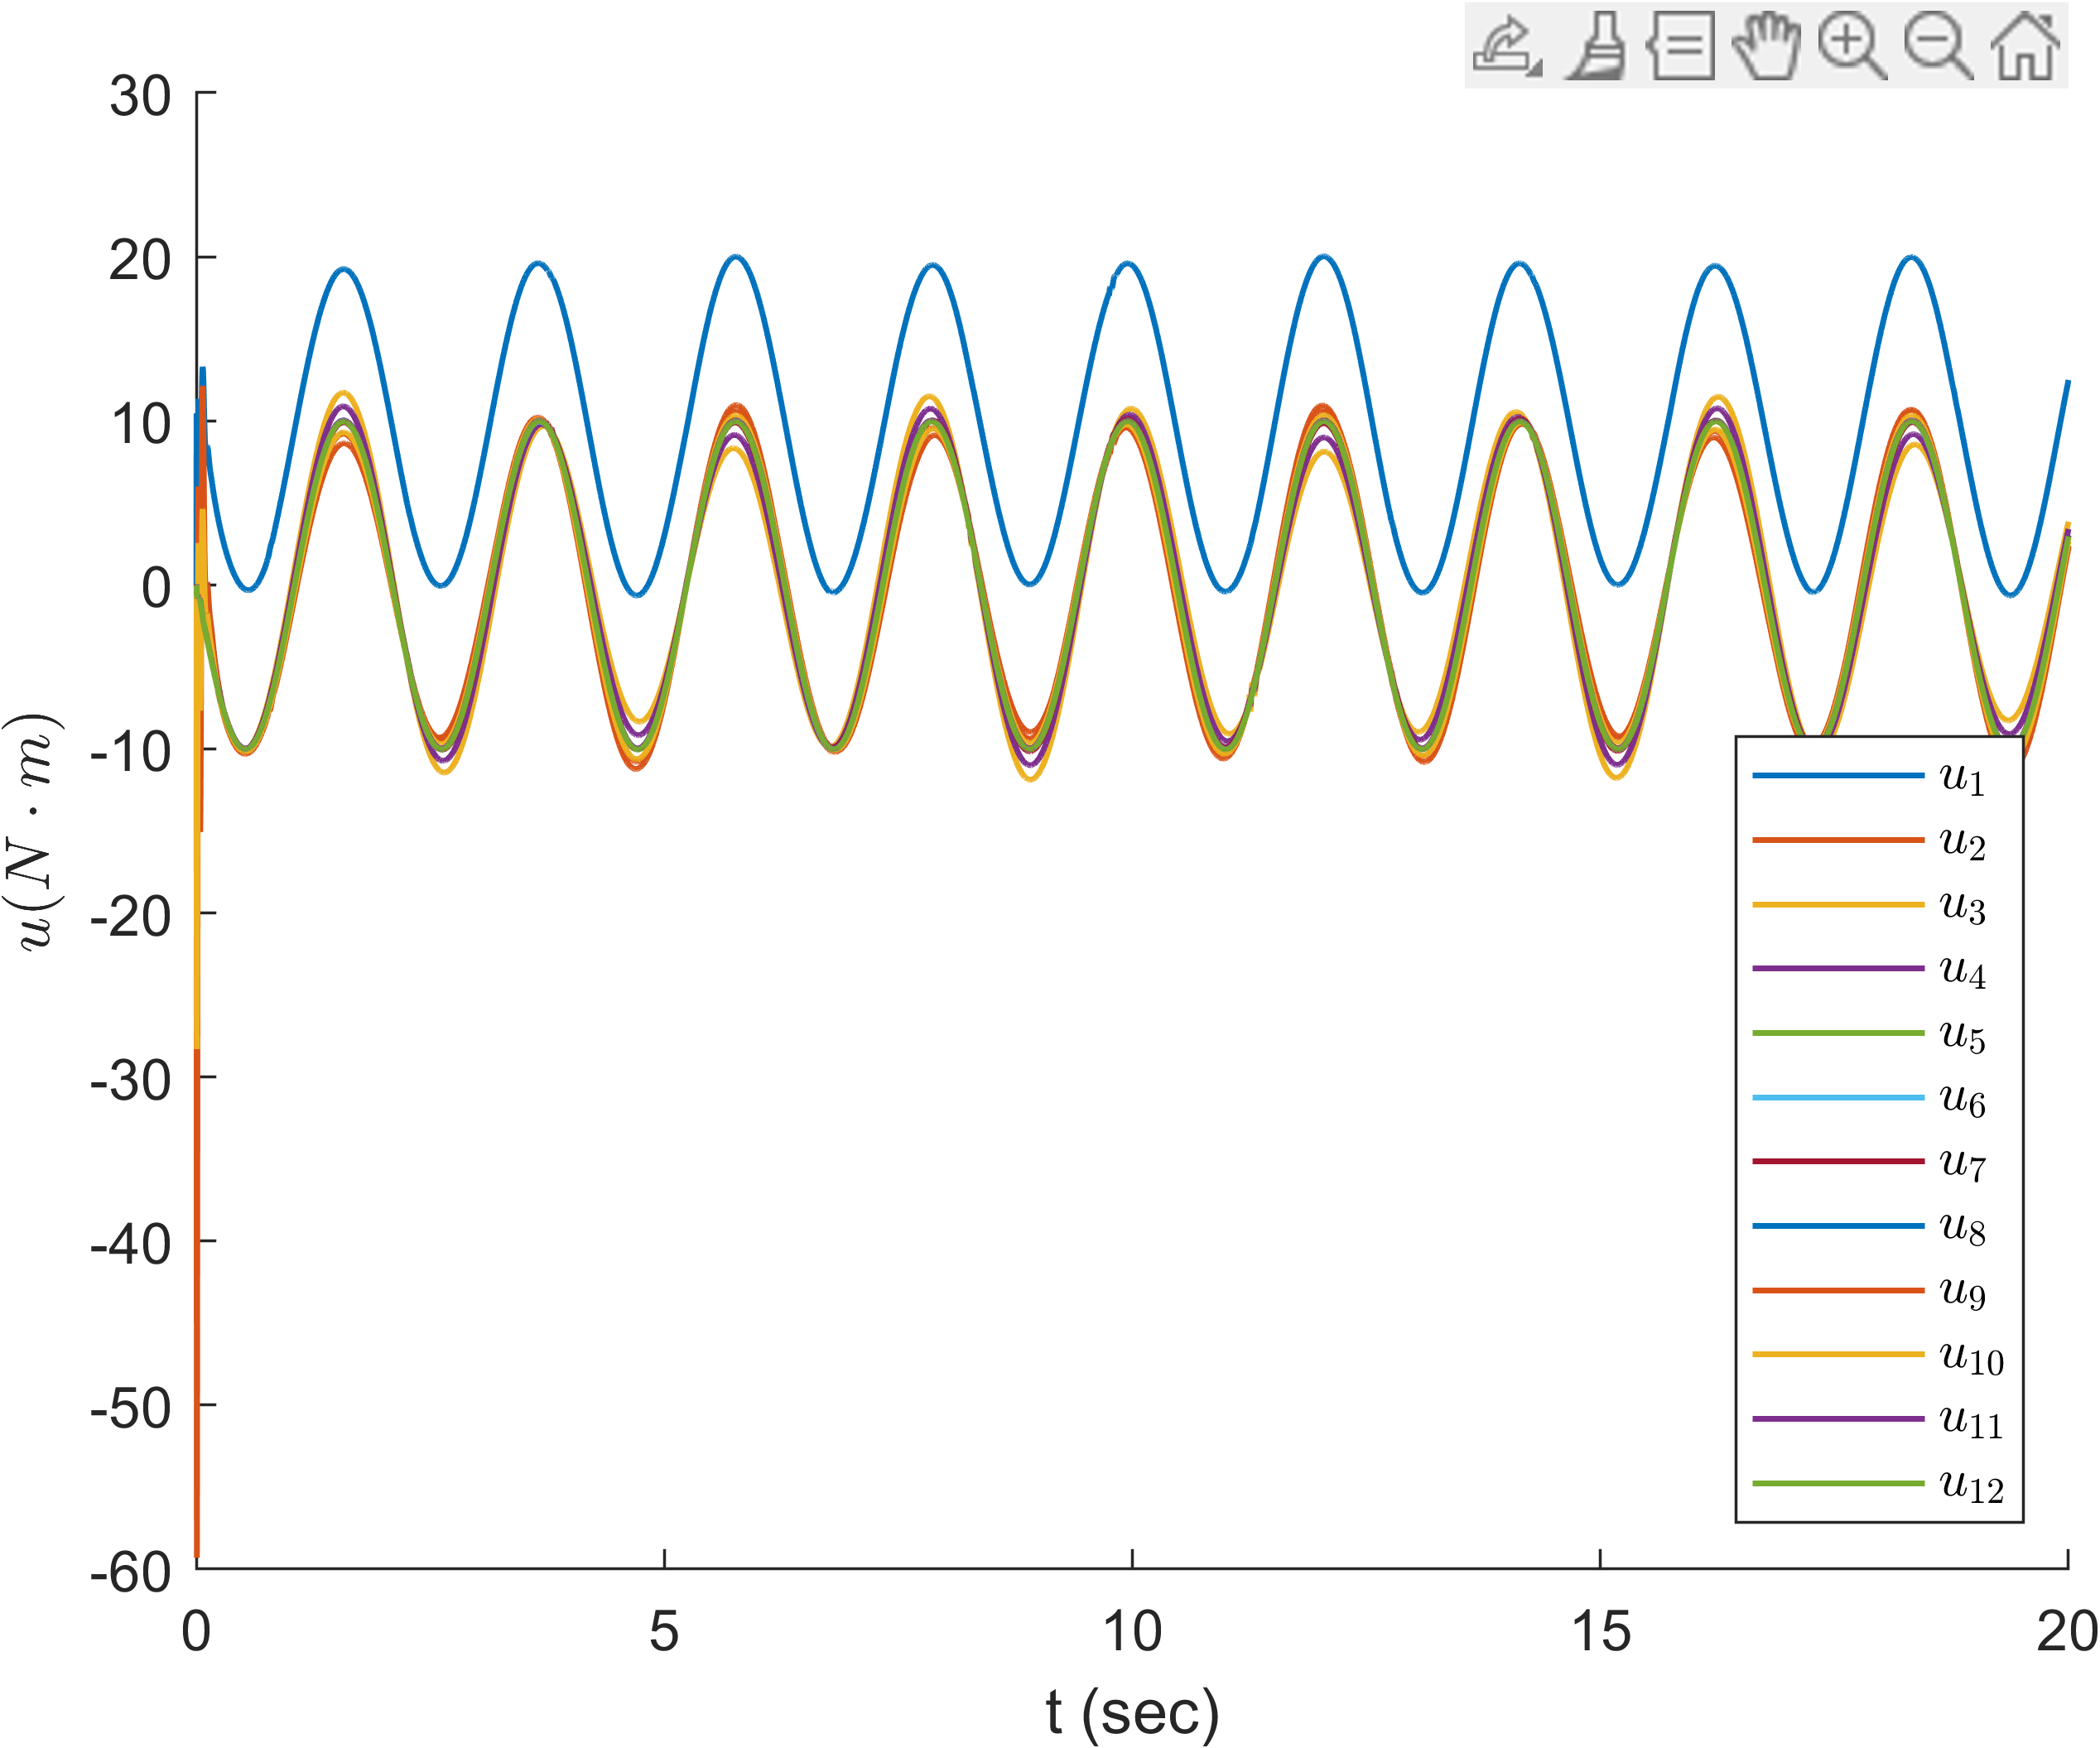
\includegraphics[scale=.57]{fig/robot (4).png}\caption{The control effort of the robot $\alpha_{1,2}$}%
    \label{fig:robot, control}
\end{figure}

In Fig. \ref{fig:UAV, state}, the tracking and estimation errors of UAV position and attitude reach the steady state all within $2$ seconds. There is a brief jitter when the sensor fault signal changes drastically, but it returns quickly to the steady state. In Fig. \ref{fig:robot, state}, the tracking and estimation errors of robot joint angles immediately reach and maintain steady state under the influence of fault signals. In Figs. \ref{fig:UAV, fa} and \ref{fig:robot, fa}, the results show that the actuator fault, i.e., feedforward control errors and disturbances, can be effectively estimated. However, in Figs. \ref{fig:UAV, fs} and \ref{fig:robot, fs}, the estimation of sensor fault has an overshot phenomenon when there is a large change and returns to a steady state after about $2$ seconds. In Figs. \ref{fig:UAV, control} and \ref{fig:robot, control}, the control efforts have high frequency and high amplitude at the initial instance due to the high gain characteristic of the robust control. After that, they maintain the sine wave shape to offset the estimated actuator fault value. Besides, it can be seen that the total force $F$ of UAV remains constant against gravity in Fig. \ref{fig:UAV, control}.
% The transient responses that occur later are caused from fault signals, especially the sensor fault. This can be inferred from the dynamic of the estimation error (\ref{eq:e_tilde}) because the value of the sensor fault affects the value of the estimation error over time $\dot{\tilde{e}}$ not only from the term $\bar{A}$ but also from the term $L\bar{C}$.

For further verification, we visualized the simulation of a hybrid team tracking in URTS and the configuration trajectory of biped robot on the online resource \cite{mySimulation}. The results again demonstrate the effectiveness of the proposed $H_\infty$ decentralized observer-based feedforward-linearized PID FTC method for agents in URTS.

\section{conclusion}
In this study, a system architecture of URTS is given for S\&R usage. This gives a holistic view of the operational framework for URTS. By decomposing the path planning process into three subprocess, i.e., path planning, behavior layer, local motion planning, some common path planning algorithm can be applied in URTS. Next, we focus on the local motion planning of UAV flying and robot walking behavior. Besides, the bridging method between the reference path designed by local motion planning and the tracking control design is also given. By a general nonlinear agent dynamics model, the tracking control problem of UAV and robot can be analysis together. Through a feedforward-linearized strategy, the nonlinear tracking control problem with external disturbances is transformed to a regulation problem with fault signals. Then, a smoothing signal model is introduced to embed the fault signals into the state vector to avoid the corruption on the agent dynamic system. After that, a robust $H_\infty$ decentralized observer-based feedforward-linearized PID FTC strategy is proposed for each agent in the hybrid URTS. To solve the robust $H_\infty$ decentralized observer-based feedforward-linearized PID FTC problem, we transform it into a LMI-constrained optimization problem by a two-step design procedure, which can be effectively solved by MATLAB LMI Toolbox. A simulation example is given to illustrate more concretely how the proposed hybrid URTS architecture actually works. Finally, the effectiveness of the proposed robust $H_\infty$ decentralized observer-based feedforward-linearized PID FTC method is also verified by the simulation results. In the future, we will...

% \nocite{*}
\bibliographystyle{IEEEtran}
\bibliography{citation}
% \begin{thebibliography}{00}
%     \bibitem{9700861} L. Kloeker, T. Moers, L. Vater, A. Zlocki, and L. Eckstein, “Utilization
%     and potentials of unmanned aerial vehicles (uavs) in the field of automated
%     driving: A survey,” in 2021 5th International Conference on Vision, Image
%     and Signal Processing (ICVISP), pp. 9–17, 2021
% \end{thebibliography}

\EOD

\end{document}